% MIT 18.03 Spring 2010. 原题编号保留; 解答与原题分离.
\originalchapter{题库一: 一阶微分方程}
\originalsection{1A: 入门与变量分离}
\begin{exercise}\label{cw:bank-1A-1}
原题1A-1. 验证下列方程具有所列解, 其中 $c_1,c_2,a$ 为常数:
\begin{enumerate}[label=\alph*)]
\item $y''-2y'+y=0$, $y=c_1e^x+c_2xe^x$.
\item $xy'+y=x\sin x$, $y=(\sin x+a)/x-\cos x$.
\end{enumerate}
\end{exercise}
\begin{solution}
官方答案译审. (a) $y'=e^x(c_1+c_2x+c_2)$, $y''=e^x(c_1+c_2x+2c_2)$, 代入即为零. (b) 在 $x\ne0$ 上, $xy=\sin x+a-x\cos x$, 故 $(xy)'=x\sin x$.
\end{solution}
\begin{exercise}\label{cw:bank-1A-2}
原题1A-2. 下列函数族实际依赖几个任意常数? $a,b,c,d,k,c_i$ 均为常数, 表面出现的常数不一定独立.
\begin{enumerate}[label=\alph*)]
\item $c_1e^{kx}$. \item $c_1e^{x+a}$. \item $c_1+c_2\cos2x+c_3\cos^2x$. \item $\ln(ax+b)+\ln(cx+d)$.
\end{enumerate}
\end{exercise}
\begin{solution}
官方答案译审. 依次为 $2,1,2,3$. (a) 非零成员的振幅与指数率可独立改变. (b) 合并为 $(c_1e^a)e^x$. (c) 用 $\cos2x=2\cos^2x-1$, 得 $(c_1-c_2)+(2c_2+c_3)\cos^2x$. (d) 在两个对数均有定义的区间, 合并为 $\ln[acx^2+(ad+bc)x+bd]$, 只涉及三个组合参数; 这三个组合在一般参数点能独立变化. 个别退化成员不会增加整个函数族的参数数目.
\end{solution}
\begin{exercise}\label{cw:bank-1A-3}
原题1A-3. 写出含定积分的显式解:
\begin{enumerate}[label=\alph*)]
\item $y'=1/(y^2\ln x)$, $y(2)=0$.
\item $y'=ye^x/x$, $y(1)=1$.
\end{enumerate}
\end{exercise}
\begin{solution}
依据官方答案补核. (a) 原题初值处右端未定义, 因而没有包含 $x=2$ 的经典解. 官方的分离计算给出形式曲线
\[
 y(x)=\sqrt[3]{3\int_2^x\frac{dt}{\ln t}}.
\]
它在 $2$ 附近连续, 在 $x\ne2$ 的两侧分别满足方程, 但 $y'(x)$ 在 $2$ 处无界, 不能称为此初值问题的经典解. (b) $\ln y=\int_1^x e^t/t\,dt$, 故 $y=\exp(\int_1^x e^t/t\,dt)$, $x>0$.
\end{solution}
\begin{exercise}\label{cw:bank-1A-4}
原题1A-4. 解初值问题:
\begin{enumerate}[label=\alph*)]
\item $y'=(xy+x)/y$, $y(2)=0$.
\item $du/dt=\sin t\cos^2u$, $u(0)=0$.
\end{enumerate}
\end{exercise}
\begin{solution}
依据官方答案补核. (a) 初值处方程未定义, 无经典解. 在 $y\ne0,-1$ 上分离得 $y-\ln|y+1|=x^2/2+C$; 经过 $(2,0)$ 的形式关系是 $y-\ln|y+1|=x^2/2-2$. 左端在 $y=0$ 附近为 $y^2/2+O(y^3)$, 故这里只产生 $x\ge2$ 一侧的分支, 其起点切线竖直. (b) $\sec^2u\,du=\sin t\,dt$, 从初值积分得 $\tan u=1-\cos t$, 因而 $u=\arctan(1-\cos t)$.
\end{solution}
\begin{exercise}\label{cw:bank-1A-5}
原题1A-5. 用变量分离求通解:
\begin{enumerate}[label=\alph*)]
\item $(y^2-2y)\,dx+x^2\,dy=0$.
\item $x\,dv/dx=\sqrt{1-v^2}$.
\item $y'=((y-1)/(x+1))^2$.
\item $dx/dt=\sqrt{1+x}/(t^2+4)$.
\end{enumerate}
\end{exercise}
\begin{solution}
官方答案译审并补齐分离时遗漏的常数解. (a) $\frac12\ln|(y-2)/y|=1/x+C$, 故 $y=2/(1-Ce^{2/x})$, 并有 $y=0$; 以上取 $x\ne0$ 的解区间. (b) $\arcsin v=\ln|x|+C$, 即 $v=\sin(\ln|x|+C)$, 必须限制在 $\cos(\ln|x|+C)\ge0$ 的区间, 因为原式平方根非负. 常数解 $v=\pm1$ 也须保留, 并可在端点与非常数分支粘接. (c) $-1/(y-1)=-1/(x+1)+C$, 即 $y=1+(x+1)/(1-C(x+1))$; 另有 $y=1$, 且 $x\ne-1$. (d) $2\sqrt{1+x}=\frac12\arctan(t/2)+C$, 所以 $x=[\frac14\arctan(t/2)+C]^2-1$, 要求括号非负; 另有 $x=-1$, 可在非负分支的零点粘接.
\end{solution}
\originalsection{1B: 一阶方程的标准方法}
\begin{exercise}\label{cw:bank-1B-1}
原题1B-1. 判定是否恰当, 对恰当方程求通解:
\begin{enumerate}[label=\alph*)]
\item $3x^2y\,dx+(x^3+y^3)\,dy=0$.
\item $(x^2-y^2)\,dx+(y^2-x^2)\,dy=0$.
\item $ve^{uv}\,du+ue^{uv}\,dv=0$.
\item $2xy\,dx-x^2\,dy=0$.
\end{enumerate}
\end{exercise}
\begin{solution}
官方答案译审. 比较 $M_y$ 与 $N_x$: (a) 均为 $3x^2$, 势函数 $x^3y+y^4/4$, 解为 $x^3y+y^4/4=C$. (b) 分别为 $-2y,-2x$, 不恰当. (c) 均为 $(1+uv)e^{uv}$, 势函数 $e^{uv}$, 解为 $e^{uv}=C$, 等价于 $uv=C_1$. (d) 分别为 $2x,-2x$, 不恰当.
\end{solution}
\begin{exercise}\label{cw:bank-1B-2}
原题1B-2. 求积分因子并解方程:
\begin{enumerate}[label=\alph*)]
\item $2x\,dx+(x^2/y)\,dy=0$.
\item $y\,dx-(x+y)\,dy=0$, $y(1)=1$.
\item $(t^2+4)\,dt+t\,dx=x\,dt$.
\item $u(du-dv)+v(du+dv)=0$, $v(0)=1$.
\end{enumerate}
\end{exercise}
\begin{solution}
官方答案译审. (a) 乘 $y$ 后为 $d(x^2y)=0$, 故 $x^2y=C$, 取原式有定义处. (b) 乘 $y^{-2}$ 后为 $d(x/y)-d(\ln|y|)=0$, 初值给 $x/y-\ln y=1$, 即 $x=y(1+\ln y)$, $y>0$. (c) 乘 $t^{-2}$, 得 $d(x/t)=(1+4/t^2)dt$, 所以 $x=t^2-4+Ct$, $t\ne0$. (d) 乘 $(u^2+v^2)^{-1}$, 在初值附近以 $u=r\sin\theta,v=r\cos\theta$ 表示, 方程变为 $d\ln r+d\theta=0$. 初值给 $\ln r+\theta=0$, 即 $r=e^{-\theta}$. 角度须连续选取; 这也给出经过 $(0,1)$ 的螺线.
\end{solution}
\begin{exercise}\label{cw:bank-1B-3}
原题1B-3. 解齐次方程:
\begin{enumerate}[label=\alph*)]
\item $y'=(2y-x)/(y+4x)$.
\item $dw/du=2uw/(u^2-w^2)$.
\item $xy\,dy-y^2\,dx=x\sqrt{x^2-y^2}\,dx$.
\end{enumerate}
\end{exercise}
\begin{solution}
官方答案译审并核对定义域. (a) 令 $z=y/x$, 则 $xz'=-(z+1)^2/(z+4)$. 积分得 $\ln|z+1|-3/(z+1)=-\ln|x|+C$, 即 $\ln|x+y|-3x/(x+y)=C$. 分离遗漏的 $y=-x$ 也是解. (b) 令 $z=w/u$, 则 $uz'=z(1+z^2)/(1-z^2)$; 积分得 $\ln|z/(1+z^2)|=\ln|u|+C$, 故 $w/(u^2+w^2)=C$. 零解含在其中, 原方程排除 $u^2=w^2$. (c) 在 $x>0$ 令 $z=y/x$, 则 $xz z'=\sqrt{1-z^2}$, 得 $\sqrt{1-z^2}=C-\ln x$. 因而 $y=\pm x\sqrt{1-(C-\ln x)^2}$, 经典非边界分支须 $0<C-\ln x<1$, 即 $|y|<|x|$ 且 $y\ne0$. 等号 $C-\ln x=1$ 对应 $y=0$ 的竖直切线端点, 不能包含为可微的 $y(x)$ 解; $C-\ln x=0$ 可与边界解相接. 在 $x<0$ 上相应为 $\sqrt{1-z^2}=C+\ln|x|$, 同样在严格内侧 $0<C+\ln|x|<1$ 取经典非边界分支. 边界直线 $y=\pm x$ 也满足原微分关系.
\end{solution}
\begin{exercise}\label{cw:bank-1B-4}
原题1B-4. 证明代换 $u=y/x^n$ 对适当的 $n$ 可把 $y'=(4+xy^2)/(x^2y)$ 化为变量可分离方程, 并求解. 提示: 先用 $u,x$ 表示 $y,y'$.
\end{exercise}
\begin{solution}
官方答案译审. 写成 $y'=y/x+4/(x^2y)$. 取 $n=1$, $y=xu$, 则 $xu'=4/(x^3u)$, 即 $u u'=4/x^4$. 所以 $u^2=C-8/(3x^3)$, $y^2=Cx^2-8/(3x)$. 取右端为正的区间和任一固定符号平方根, 且 $x,y\ne0$.
\end{solution}
\begin{exercise}\label{cw:bank-1B-5}
原题1B-5. 求通解或满足初值的解:
\begin{enumerate}[label=\alph*)]
\item $xy'+2y=x$.
\item $dx/dt-x\tan t=t/\cos t$, $x(0)=0$.
\item $(x^2-1)y'=1-2xy$.
\item $3v\,dt=t(dt-dv)$, $v(1)=1/4$.
\end{enumerate}
\end{exercise}
\begin{solution}
官方答案译审. (a) 乘积分因子 $x^2$: $(x^2y)'=x^2$, 得 $y=x/3+C/x^2$. (b) $(x\cos t)'=t$, 得 $x=t^2/(2\cos t)$, 初值区间 $|t|<\pi/2$. (c) $[(x^2-1)y]'=1$, 得 $y=(x+C)/(x^2-1)$, 可消去的奇点需另检查原式. (d) $v'+3v/t=1$, 故 $(t^3v)'=t^3$, $v=t/4+C/t^3$. 初值使 $C=0$.
\end{solution}
\begin{exercise}\label{cw:bank-1B-6}
原题1B-6. 设 $a>0$, $r(t)\to0$ ($t\to\infty$). 证明 $x'+ax=r(t)$ 的每个解均趋于零. 提示: 可用洛必达法则.
\end{exercise}
\begin{solution}
官方思路译审并补齐极限论证. 积分因子给
\[
 x(t)=e^{-a(t-t_0)}x(t_0)+\int_{t_0}^t e^{-a(t-s)}r(s)\,ds.
\]
给定 $\varepsilon>0$, 取 $T$ 使 $s\ge T$ 时 $|r(s)|\le a\varepsilon$. 积分的 $[t_0,T]$ 部分随 $t\to\infty$ 趋零, $[T,t]$ 部分绝对值至多 $\varepsilon(1-e^{-a(t-T)})$. 所以 $\limsup|x(t)|\le\varepsilon$, 再令 $\varepsilon\to0$. 这避免在积分分子可能不趋于无穷时误用洛必达法则.
\end{solution}
\begin{exercise}\label{cw:bank-1B-7}
原题1B-7. 解 $y'=y/(y^3+x)$. 提示: 考察 $dx/dy$.
\end{exercise}
\begin{solution}
官方答案译审. 对非零解交换变量: $dx/dy-x/y=y^2$. 乘 $1/y$ 得 $d(x/y)/dy=y$, 故 $x=y^3/2+Cy$. 此关系只在 $y^3+x\ne0$ 且能局部表示为 $y(x)$ 时成立. 另有 $y=0$ ($x\ne0$).
\end{solution}
\begin{exercise}\label{cw:bank-1B-8}
原题1B-8. Bernoulli 方程 $y'+p(x)y=q(x)y^n$, $n\ne1$. 证明代换 $u=y^{1-n}$ 将其化为线性方程. 提示: 先除以 $y^n$.
\end{exercise}
\begin{solution}
官方答案译审. 在实幂有定义且 $y\ne0$ 的区间, $u'=(1-n)y^{-n}y'$, 所以 $u'+(1-n)pu=(1-n)q$. 代换前须另检查零解; 它不一定属于实幂方程的定义域.
\end{solution}
\begin{exercise}\label{cw:bank-1B-9}
原题1B-9. 用1B-8的方法解:
\begin{enumerate}[label=\alph*)]
\item $y'+y=2xy^2$. \item $x^2y'-y^3=xy$.
\end{enumerate}
\end{exercise}
\begin{solution}
官方答案译审. (a) $u=1/y$ 满足 $u'-u=-2x$, 故 $u=2x+2+Ce^x$, $y=(2x+2+Ce^x)^{-1}$; 另有 $y=0$. (b) $u=y^{-2}$ 满足 $u'+2u/x=-2/x^2$, 得 $(x^2u)'=-2$, 故 $y=\pm x/\sqrt{C-2x}$, 在 $C-2x>0$, $x\ne0$ 上取固定分支; 另有 $y=0$.
\end{solution}
\begin{exercise}\label{cw:bank-1B-10}
原题1B-10. Riccati 方程 $y'=A(x)+B(x)y+C(x)y^2$ 一般不能用初等函数求解.
\begin{enumerate}[label=\alph*)]
\item 已知一个解 $y_1$, 证明通解可写成 $y=y_1+u$, 其中 $u$ 满足某个 Bernoulli 方程.
\item 据此解 $y'=1-x^2+y^2$.
\end{enumerate}
\end{exercise}
\begin{solution}
官方答案译审. (a) 代入并减去 $y_1$ 的方程, 得 $u'=(B+2Cy_1)u+Cu^2$. (b) $y_1=x$ 是特解. 若 $u\ne0$, 令 $w=1/u$, 得 $w'+2xw=-1$, 故
\[
 y=x+\frac{e^{x^2}}{K-\int_0^x e^{t^2}\,dt}.
\]
分母非零时有效; 原特解 $y=x$ 也要保留.
\end{solution}
\begin{exercise}\label{cw:bank-1B-11}
原题1B-11. 解下列二阶自治方程. 自治表示独立变量没有显式出现在方程中.
\begin{enumerate}[label=\alph*)]
\item $y''=a^2y$. \item $yy''=(y')^2$. \item $y''=y'(1+3y^2)$, $y(0)=1$, $y'(0)=2$.
\end{enumerate}
\end{exercise}
\begin{solution}
官方答案译审并补齐退化解. 以 $v=y'$ 为 $y$ 的函数, 则 $y''=v\,dv/dy$. (a) 积分得 $v^2=a^2y^2+C$, 最终 $y=Ae^{ax}+Be^{-ax}$ ($a\ne0$); $a=0$ 时 $y=Ax+B$. (b) 在 $y\ne0$ 时 $(y'/y)'=0$, 所以 $y=Ae^{kx}$. 零解也满足; 非零解不能有限时达到零, 因而没有额外跨零分支. (c) $dv/dy=1+3y^2$, 得 $v=y+y^3+C$; 初值给 $C=0$. 分离后 $y/\sqrt{1+y^2}=e^x/\sqrt2$, 因而 $y=e^x/\sqrt{2-e^{2x}}$, 最大初值区间为 $x<\frac12\ln2$.
\end{solution}
\begin{exercise}\label{cw:bank-1B-12}
原题1B-12. 只说明各式的类型和求解方法, 不必求解; 某些式可用多种方法.
\begin{enumerate}[label=\arabic*.]
\item $(x^3+y)dx+xdy=0$. \item $dy/dt+2ty-e^{-t}=0$.
\item $y'=(x^2-y^2)/(5xy)$. \item $(1+2p)dq+(2-q)dp=0$.
\item $\cos x\,dy=(y\sin x+e^x)dx$. \item $x\tan y\,y'=-1$.
\item $y'=y/x+1/y$. \item $dv/du=e^{2u+3v}$.
\item $xy'=y+xe^{y/x}$. \item $xy'-y=x^2\sin x$.
\item $y'=(x+e^y)^{-1}$. \item $y'+2y/x-y^2/x=0$.
\item $dx/dy=-x(2x^2y+\cos y)/(3x^2y^2+\sin y)$.
\item $y'+3y=e^{-3t}$. \item $x\,dy/dx-y=\sqrt{x^2+y^2}$.
\item $(y'-1)/x^2=1$. \item $xy'-2y+y^2=x^4$.
\item $y''=y(y+1)/y'$. \item $t\,ds/dt=s(1-\ln t+\ln s)$.
\item $dy/dx=(3-2y)/(2x+y+1)$. \item $x^2y'+xy+y^2=0$.
\item $y'\tan(x+y)=1-\tan(x+y)$. \item $y\,ds-3s\,dy=y^4dy$.
\item $du=-(1+u\cos^2t)/(t\cos^2t)\,dt$.
\item $y'+y^2+(2x+1)y+1+x+x^2=0$. \item $y''+x^2y'+3x^3=\sin x$.
\end{enumerate}
\end{exercise}
\begin{solution}
官方答案译审. 按题号依次为:
\begin{enumerate}[label=\arabic*.]
\item 恰当, 或以 $y$ 为未知量的线性式.
\item 线性, 积分因子 $e^{t^2}$.
\item 齐次, 令 $y=xz$.
\item 可分离; 也分别对 $p$ 或 $q$ 线性.
\item 恰当, 或线性.
\item 可分离.
\item Bernoulli, $n=-1$, 令 $u=y^2$.
\item 可分离.
\item 齐次, 令 $z=y/x$.
\item 线性, 积分因子 $1/x$.
\item 交换变量后 $dx/dy=x+e^y$, 线性.
\item 可分离或 Bernoulli.
\item 写成 $(3x^2y^2+\sin y)dx+x(2x^2y+\cos y)dy=0$, 恰当.
\item 对 $t$ 的线性式.
\item 在 $x>0$ 或 $x<0$ 分别令 $y=xz$, 化为可分离式.
\item 直接积分.
\item Riccati, 已知特解 $y=x^2$, 再令 $y=x^2+u$.
\item 自治降阶, 令 $v=y'$, 得 $v^2dv/dy=y(y+1)$.
\item 在 $s,t>0$ 上令 $s=tz$, 利用 $\ln s-\ln t=\ln z$ 分离.
\item 写成 $(2y-3)dx+(2x+y+1)dy=0$, 恰当.
\item Bernoulli, $n=2$.
\item 令 $u=x+y$, 则 $u'=\cot u$, 可分离.
\item 以 $y$ 为独立变量、$s$ 为未知函数的线性式.
\item 以 $t$ 为独立变量、$u$ 为未知函数的线性式.
\item Riccati, 特解 $y=-x$; 或令 $u=x+y$, 得 $u'+u^2+u=0$.
\item 令 $v=y'$, 得一阶线性式 $v'+x^2v=\sin x-3x^3$.
\end{enumerate}
\end{solution}
\originalsection{1C: 图解与数值方法}
\begin{exercise}\label{cw:bank-1C-1}
原题1C-1. 对各式选约五条等倾线绘方向场, 在两坐标均为 $[-2,2]$ 的正方形内画若干积分曲线, 并完成附加要求.
\begin{enumerate}[label=\alph*)]
\item $y'=-y/x$: 求精确解并比较.
\item $y'=2x+y$: 找出图形同时是等倾线的解, 并用计算验证.
\item $y'=x-y$: 同(b).
\item $y'=x^2+y^2-1$.
\item $y'=1/(x+y)$: 改用 $[-3,3]^2$, 画经过 $(0,0),(-1,1),(0,-2)$ 的积分曲线. 它们会越过 $y=-x-1$ 吗? 用解曲线不相交原理解释.
\end{enumerate}
\end{exercise}
\begin{solution}
官方答案译审并补核奇点. 等倾线分别为 (a) $y=-cx$, (b) $y=c-2x$, (c) $y=x-c$, (d) $x^2+y^2=1+c$, (e) $y=-x+1/c$. (a) $y=C/x$. (b) 解族 $y=Ce^x-2x-2$, $C=0$ 给直线 $y=-2x-2$, 其斜率和右端都为 $-2$. (c) $y=Ce^{-x}+x-1$, $C=0$ 给等倾线解 $y=x-1$.

(e) 令 $z=x+y$, 则 $z'=1+1/z$, 因而 $x=z-\ln|z+1|+C$, 即 $y-\ln|x+y+1|=C_1$. 经过三点的形式常数依次为 $0,1,-2$. 前两点位于 $x+y=0$ 的奇线, 没有以该点为初值的经典解; 图中画的是该点附近的几何分支, 起点有竖直切线. $y=-x-1$ 本身是经典解, 其附近右端光滑, 所以其他经典分支不能与它相交.
\begin{center}\begin{tikzpicture}\begin{axis}[width=6.8cm,height=6.8cm,axis lines=middle,xmin=-2,xmax=2,ymin=-2,ymax=2,xlabel=$x$,ylabel=$y$,title={(a)},clip=true]
\addplot[black,dashed,domain=-2:2] {--2*x};
\addplot[black,dashed,domain=-2:2] {--1*x};
\addplot[black,dashed,domain=-2:2] {-0*x};
\addplot[black,dashed,domain=-2:2] {-1*x};
\addplot[black,dashed,domain=-2:2] {-2*x};
\draw[gray] (axis cs:-2.08485,-1.91515)--(axis cs:-1.91515,-2.08485);
\draw[gray] (axis cs:-2.09600,-1.42800)--(axis cs:-1.90400,-1.57200);
\draw[gray] (axis cs:-2.10733,-0.94633)--(axis cs:-1.89267,-1.05367);
\draw[gray] (axis cs:-2.11642,-0.47090)--(axis cs:-1.88358,-0.52910);
\draw[gray] (axis cs:-2.12000,0.00000)--(axis cs:-1.88000,0.00000);
\draw[gray] (axis cs:-2.11642,0.47090)--(axis cs:-1.88358,0.52910);
\draw[gray] (axis cs:-2.10733,0.94633)--(axis cs:-1.89267,1.05367);
\draw[gray] (axis cs:-2.09600,1.42800)--(axis cs:-1.90400,1.57200);
\draw[gray] (axis cs:-2.08485,1.91515)--(axis cs:-1.91515,2.08485);
\draw[gray] (axis cs:-1.57200,-1.90400)--(axis cs:-1.42800,-2.09600);
\draw[gray] (axis cs:-1.58485,-1.41515)--(axis cs:-1.41515,-1.58485);
\draw[gray] (axis cs:-1.59985,-0.93344)--(axis cs:-1.40015,-1.06656);
\draw[gray] (axis cs:-1.61384,-0.46205)--(axis cs:-1.38616,-0.53795);
\draw[gray] (axis cs:-1.62000,0.00000)--(axis cs:-1.38000,0.00000);
\draw[gray] (axis cs:-1.61384,0.46205)--(axis cs:-1.38616,0.53795);
\draw[gray] (axis cs:-1.59985,0.93344)--(axis cs:-1.40015,1.06656);
\draw[gray] (axis cs:-1.58485,1.41515)--(axis cs:-1.41515,1.58485);
\draw[gray] (axis cs:-1.57200,1.90400)--(axis cs:-1.42800,2.09600);
\draw[gray] (axis cs:-1.05367,-1.89267)--(axis cs:-0.94633,-2.10733);
\draw[gray] (axis cs:-1.06656,-1.40015)--(axis cs:-0.93344,-1.59985);
\draw[gray] (axis cs:-1.08485,-0.91515)--(axis cs:-0.91515,-1.08485);
\draw[gray] (axis cs:-1.10733,-0.44633)--(axis cs:-0.89267,-0.55367);
\draw[gray] (axis cs:-1.12000,0.00000)--(axis cs:-0.88000,0.00000);
\draw[gray] (axis cs:-1.10733,0.44633)--(axis cs:-0.89267,0.55367);
\draw[gray] (axis cs:-1.08485,0.91515)--(axis cs:-0.91515,1.08485);
\draw[gray] (axis cs:-1.06656,1.40015)--(axis cs:-0.93344,1.59985);
\draw[gray] (axis cs:-1.05367,1.89267)--(axis cs:-0.94633,2.10733);
\draw[gray] (axis cs:-0.52910,-1.88358)--(axis cs:-0.47090,-2.11642);
\draw[gray] (axis cs:-0.53795,-1.38616)--(axis cs:-0.46205,-1.61384);
\draw[gray] (axis cs:-0.55367,-0.89267)--(axis cs:-0.44633,-1.10733);
\draw[gray] (axis cs:-0.58485,-0.41515)--(axis cs:-0.41515,-0.58485);
\draw[gray] (axis cs:-0.62000,0.00000)--(axis cs:-0.38000,0.00000);
\draw[gray] (axis cs:-0.58485,0.41515)--(axis cs:-0.41515,0.58485);
\draw[gray] (axis cs:-0.55367,0.89267)--(axis cs:-0.44633,1.10733);
\draw[gray] (axis cs:-0.53795,1.38616)--(axis cs:-0.46205,1.61384);
\draw[gray] (axis cs:-0.52910,1.88358)--(axis cs:-0.47090,2.11642);
\draw[gray] (axis cs:0.47090,-2.11642)--(axis cs:0.52910,-1.88358);
\draw[gray] (axis cs:0.46205,-1.61384)--(axis cs:0.53795,-1.38616);
\draw[gray] (axis cs:0.44633,-1.10733)--(axis cs:0.55367,-0.89267);
\draw[gray] (axis cs:0.41515,-0.58485)--(axis cs:0.58485,-0.41515);
\draw[gray] (axis cs:0.38000,0.00000)--(axis cs:0.62000,0.00000);
\draw[gray] (axis cs:0.41515,0.58485)--(axis cs:0.58485,0.41515);
\draw[gray] (axis cs:0.44633,1.10733)--(axis cs:0.55367,0.89267);
\draw[gray] (axis cs:0.46205,1.61384)--(axis cs:0.53795,1.38616);
\draw[gray] (axis cs:0.47090,2.11642)--(axis cs:0.52910,1.88358);
\draw[gray] (axis cs:0.94633,-2.10733)--(axis cs:1.05367,-1.89267);
\draw[gray] (axis cs:0.93344,-1.59985)--(axis cs:1.06656,-1.40015);
\draw[gray] (axis cs:0.91515,-1.08485)--(axis cs:1.08485,-0.91515);
\draw[gray] (axis cs:0.89267,-0.55367)--(axis cs:1.10733,-0.44633);
\draw[gray] (axis cs:0.88000,0.00000)--(axis cs:1.12000,0.00000);
\draw[gray] (axis cs:0.89267,0.55367)--(axis cs:1.10733,0.44633);
\draw[gray] (axis cs:0.91515,1.08485)--(axis cs:1.08485,0.91515);
\draw[gray] (axis cs:0.93344,1.59985)--(axis cs:1.06656,1.40015);
\draw[gray] (axis cs:0.94633,2.10733)--(axis cs:1.05367,1.89267);
\draw[gray] (axis cs:1.42800,-2.09600)--(axis cs:1.57200,-1.90400);
\draw[gray] (axis cs:1.41515,-1.58485)--(axis cs:1.58485,-1.41515);
\draw[gray] (axis cs:1.40015,-1.06656)--(axis cs:1.59985,-0.93344);
\draw[gray] (axis cs:1.38616,-0.53795)--(axis cs:1.61384,-0.46205);
\draw[gray] (axis cs:1.38000,0.00000)--(axis cs:1.62000,0.00000);
\draw[gray] (axis cs:1.38616,0.53795)--(axis cs:1.61384,0.46205);
\draw[gray] (axis cs:1.40015,1.06656)--(axis cs:1.59985,0.93344);
\draw[gray] (axis cs:1.41515,1.58485)--(axis cs:1.58485,1.41515);
\draw[gray] (axis cs:1.42800,2.09600)--(axis cs:1.57200,1.90400);
\draw[gray] (axis cs:1.91515,-2.08485)--(axis cs:2.08485,-1.91515);
\draw[gray] (axis cs:1.90400,-1.57200)--(axis cs:2.09600,-1.42800);
\draw[gray] (axis cs:1.89267,-1.05367)--(axis cs:2.10733,-0.94633);
\draw[gray] (axis cs:1.88358,-0.52910)--(axis cs:2.11642,-0.47090);
\draw[gray] (axis cs:1.88000,0.00000)--(axis cs:2.12000,0.00000);
\draw[gray] (axis cs:1.88358,0.52910)--(axis cs:2.11642,0.47090);
\draw[gray] (axis cs:1.89267,1.05367)--(axis cs:2.10733,0.94633);
\draw[gray] (axis cs:1.90400,1.57200)--(axis cs:2.09600,1.42800);
\draw[gray] (axis cs:1.91515,2.08485)--(axis cs:2.08485,1.91515);
\addplot[main,domain=-2.00:-0.08,samples=70] {-1.00/x};
\addplot[main,domain=0.08:2.00,samples=70] {-1.00/x};
\addplot[main,domain=-2.00:-0.08,samples=70] {-0.40/x};
\addplot[main,domain=0.08:2.00,samples=70] {-0.40/x};
\addplot[main,domain=-2.00:-0.08,samples=70] {0.00/x};
\addplot[main,domain=0.08:2.00,samples=70] {0.00/x};
\addplot[main,domain=-2.00:-0.08,samples=70] {0.40/x};
\addplot[main,domain=0.08:2.00,samples=70] {0.40/x};
\addplot[main,domain=-2.00:-0.08,samples=70] {1.00/x};
\addplot[main,domain=0.08:2.00,samples=70] {1.00/x};
\end{axis}\end{tikzpicture}\end{center}
\begin{center}\begin{tikzpicture}\begin{axis}[width=6.8cm,height=6.8cm,axis lines=middle,xmin=-2,xmax=2,ymin=-2,ymax=2,xlabel=$x$,ylabel=$y$,title={(b)},clip=true]
\addplot[black,dashed,domain=-2:2] {-2-2*x};
\addplot[black,dashed,domain=-2:2] {-1-2*x};
\addplot[black,dashed,domain=-2:2] {0-2*x};
\addplot[black,dashed,domain=-2:2] {1-2*x};
\addplot[black,dashed,domain=-2:2] {2-2*x};
\draw[gray] (axis cs:-2.01973,-1.88163)--(axis cs:-1.98027,-2.11837);
\draw[gray] (axis cs:-2.02147,-1.38194)--(axis cs:-1.97853,-1.61806);
\draw[gray] (axis cs:-2.02353,-0.88233)--(axis cs:-1.97647,-1.11767);
\draw[gray] (axis cs:-2.02603,-0.38286)--(axis cs:-1.97397,-0.61714);
\draw[gray] (axis cs:-2.02910,0.11642)--(axis cs:-1.97090,-0.11642);
\draw[gray] (axis cs:-2.03297,0.61538)--(axis cs:-1.96703,0.38462);
\draw[gray] (axis cs:-2.03795,1.11384)--(axis cs:-1.96205,0.88616);
\draw[gray] (axis cs:-2.04457,1.61142)--(axis cs:-1.95543,1.38858);
\draw[gray] (axis cs:-2.05367,2.10733)--(axis cs:-1.94633,1.89267);
\draw[gray] (axis cs:-1.52353,-1.88233)--(axis cs:-1.47647,-2.11767);
\draw[gray] (axis cs:-1.52603,-1.38286)--(axis cs:-1.47397,-1.61714);
\draw[gray] (axis cs:-1.52910,-0.88358)--(axis cs:-1.47090,-1.11642);
\draw[gray] (axis cs:-1.53297,-0.38462)--(axis cs:-1.46703,-0.61538);
\draw[gray] (axis cs:-1.53795,0.11384)--(axis cs:-1.46205,-0.11384);
\draw[gray] (axis cs:-1.54457,0.61142)--(axis cs:-1.45543,0.38858);
\draw[gray] (axis cs:-1.55367,1.10733)--(axis cs:-1.44633,0.89267);
\draw[gray] (axis cs:-1.56656,1.59985)--(axis cs:-1.43344,1.40015);
\draw[gray] (axis cs:-1.58485,2.08485)--(axis cs:-1.41515,1.91515);
\draw[gray] (axis cs:-1.02910,-1.88358)--(axis cs:-0.97090,-2.11642);
\draw[gray] (axis cs:-1.03297,-1.38462)--(axis cs:-0.96703,-1.61538);
\draw[gray] (axis cs:-1.03795,-0.88616)--(axis cs:-0.96205,-1.11384);
\draw[gray] (axis cs:-1.04457,-0.38858)--(axis cs:-0.95543,-0.61142);
\draw[gray] (axis cs:-1.05367,0.10733)--(axis cs:-0.94633,-0.10733);
\draw[gray] (axis cs:-1.06656,0.59985)--(axis cs:-0.93344,0.40015);
\draw[gray] (axis cs:-1.08485,1.08485)--(axis cs:-0.91515,0.91515);
\draw[gray] (axis cs:-1.10733,1.55367)--(axis cs:-0.89267,1.44633);
\draw[gray] (axis cs:-1.12000,2.00000)--(axis cs:-0.88000,2.00000);
\draw[gray] (axis cs:-0.53795,-1.88616)--(axis cs:-0.46205,-2.11384);
\draw[gray] (axis cs:-0.54457,-1.38858)--(axis cs:-0.45543,-1.61142);
\draw[gray] (axis cs:-0.55367,-0.89267)--(axis cs:-0.44633,-1.10733);
\draw[gray] (axis cs:-0.56656,-0.40015)--(axis cs:-0.43344,-0.59985);
\draw[gray] (axis cs:-0.58485,0.08485)--(axis cs:-0.41515,-0.08485);
\draw[gray] (axis cs:-0.60733,0.55367)--(axis cs:-0.39267,0.44633);
\draw[gray] (axis cs:-0.62000,1.00000)--(axis cs:-0.38000,1.00000);
\draw[gray] (axis cs:-0.60733,1.44633)--(axis cs:-0.39267,1.55367);
\draw[gray] (axis cs:-0.58485,1.91515)--(axis cs:-0.41515,2.08485);
\draw[gray] (axis cs:-0.05367,-1.89267)--(axis cs:0.05367,-2.10733);
\draw[gray] (axis cs:-0.06656,-1.40015)--(axis cs:0.06656,-1.59985);
\draw[gray] (axis cs:-0.08485,-0.91515)--(axis cs:0.08485,-1.08485);
\draw[gray] (axis cs:-0.10733,-0.44633)--(axis cs:0.10733,-0.55367);
\draw[gray] (axis cs:-0.12000,0.00000)--(axis cs:0.12000,0.00000);
\draw[gray] (axis cs:-0.10733,0.44633)--(axis cs:0.10733,0.55367);
\draw[gray] (axis cs:-0.08485,0.91515)--(axis cs:0.08485,1.08485);
\draw[gray] (axis cs:-0.06656,1.40015)--(axis cs:0.06656,1.59985);
\draw[gray] (axis cs:-0.05367,1.89267)--(axis cs:0.05367,2.10733);
\draw[gray] (axis cs:0.41515,-1.91515)--(axis cs:0.58485,-2.08485);
\draw[gray] (axis cs:0.39267,-1.44633)--(axis cs:0.60733,-1.55367);
\draw[gray] (axis cs:0.38000,-1.00000)--(axis cs:0.62000,-1.00000);
\draw[gray] (axis cs:0.39267,-0.55367)--(axis cs:0.60733,-0.44633);
\draw[gray] (axis cs:0.41515,-0.08485)--(axis cs:0.58485,0.08485);
\draw[gray] (axis cs:0.43344,0.40015)--(axis cs:0.56656,0.59985);
\draw[gray] (axis cs:0.44633,0.89267)--(axis cs:0.55367,1.10733);
\draw[gray] (axis cs:0.45543,1.38858)--(axis cs:0.54457,1.61142);
\draw[gray] (axis cs:0.46205,1.88616)--(axis cs:0.53795,2.11384);
\draw[gray] (axis cs:0.88000,-2.00000)--(axis cs:1.12000,-2.00000);
\draw[gray] (axis cs:0.89267,-1.55367)--(axis cs:1.10733,-1.44633);
\draw[gray] (axis cs:0.91515,-1.08485)--(axis cs:1.08485,-0.91515);
\draw[gray] (axis cs:0.93344,-0.59985)--(axis cs:1.06656,-0.40015);
\draw[gray] (axis cs:0.94633,-0.10733)--(axis cs:1.05367,0.10733);
\draw[gray] (axis cs:0.95543,0.38858)--(axis cs:1.04457,0.61142);
\draw[gray] (axis cs:0.96205,0.88616)--(axis cs:1.03795,1.11384);
\draw[gray] (axis cs:0.96703,1.38462)--(axis cs:1.03297,1.61538);
\draw[gray] (axis cs:0.97090,1.88358)--(axis cs:1.02910,2.11642);
\draw[gray] (axis cs:1.41515,-2.08485)--(axis cs:1.58485,-1.91515);
\draw[gray] (axis cs:1.43344,-1.59985)--(axis cs:1.56656,-1.40015);
\draw[gray] (axis cs:1.44633,-1.10733)--(axis cs:1.55367,-0.89267);
\draw[gray] (axis cs:1.45543,-0.61142)--(axis cs:1.54457,-0.38858);
\draw[gray] (axis cs:1.46205,-0.11384)--(axis cs:1.53795,0.11384);
\draw[gray] (axis cs:1.46703,0.38462)--(axis cs:1.53297,0.61538);
\draw[gray] (axis cs:1.47090,0.88358)--(axis cs:1.52910,1.11642);
\draw[gray] (axis cs:1.47397,1.38286)--(axis cs:1.52603,1.61714);
\draw[gray] (axis cs:1.47647,1.88233)--(axis cs:1.52353,2.11767);
\draw[gray] (axis cs:1.94633,-2.10733)--(axis cs:2.05367,-1.89267);
\draw[gray] (axis cs:1.95543,-1.61142)--(axis cs:2.04457,-1.38858);
\draw[gray] (axis cs:1.96205,-1.11384)--(axis cs:2.03795,-0.88616);
\draw[gray] (axis cs:1.96703,-0.61538)--(axis cs:2.03297,-0.38462);
\draw[gray] (axis cs:1.97090,-0.11642)--(axis cs:2.02910,0.11642);
\draw[gray] (axis cs:1.97397,0.38286)--(axis cs:2.02603,0.61714);
\draw[gray] (axis cs:1.97647,0.88233)--(axis cs:2.02353,1.11767);
\draw[gray] (axis cs:1.97853,1.38194)--(axis cs:2.02147,1.61806);
\draw[gray] (axis cs:1.98027,1.88163)--(axis cs:2.01973,2.11837);
\addplot[main,domain=-2:2,samples=70] {-1.00*exp(x)-2*x-2};
\addplot[main,domain=-2:2,samples=70] {0.00*exp(x)-2*x-2};
\addplot[main,domain=-2:2,samples=70] {0.30*exp(x)-2*x-2};
\addplot[main,domain=-2:2,samples=70] {1.00*exp(x)-2*x-2};
\addplot[main,domain=-2:2,samples=70] {2.00*exp(x)-2*x-2};
\end{axis}\end{tikzpicture}\end{center}
\begin{center}\begin{tikzpicture}\begin{axis}[width=6.8cm,height=6.8cm,axis lines=middle,xmin=-2,xmax=2,ymin=-2,ymax=2,xlabel=$x$,ylabel=$y$,title={(c)},clip=true]
\addplot[black,dashed,domain=-2:2] {x--2};
\addplot[black,dashed,domain=-2:2] {x--1};
\addplot[black,dashed,domain=-2:2] {x-0};
\addplot[black,dashed,domain=-2:2] {x-1};
\addplot[black,dashed,domain=-2:2] {x-2};
\draw[gray] (axis cs:-2.12000,-2.00000)--(axis cs:-1.88000,-2.00000);
\draw[gray] (axis cs:-2.10733,-1.44633)--(axis cs:-1.89267,-1.55367);
\draw[gray] (axis cs:-2.08485,-0.91515)--(axis cs:-1.91515,-1.08485);
\draw[gray] (axis cs:-2.06656,-0.40015)--(axis cs:-1.93344,-0.59985);
\draw[gray] (axis cs:-2.05367,0.10733)--(axis cs:-1.94633,-0.10733);
\draw[gray] (axis cs:-2.04457,0.61142)--(axis cs:-1.95543,0.38858);
\draw[gray] (axis cs:-2.03795,1.11384)--(axis cs:-1.96205,0.88616);
\draw[gray] (axis cs:-2.03297,1.61538)--(axis cs:-1.96703,1.38462);
\draw[gray] (axis cs:-2.02910,2.11642)--(axis cs:-1.97090,1.88358);
\draw[gray] (axis cs:-1.60733,-2.05367)--(axis cs:-1.39267,-1.94633);
\draw[gray] (axis cs:-1.62000,-1.50000)--(axis cs:-1.38000,-1.50000);
\draw[gray] (axis cs:-1.60733,-0.94633)--(axis cs:-1.39267,-1.05367);
\draw[gray] (axis cs:-1.58485,-0.41515)--(axis cs:-1.41515,-0.58485);
\draw[gray] (axis cs:-1.56656,0.09985)--(axis cs:-1.43344,-0.09985);
\draw[gray] (axis cs:-1.55367,0.60733)--(axis cs:-1.44633,0.39267);
\draw[gray] (axis cs:-1.54457,1.11142)--(axis cs:-1.45543,0.88858);
\draw[gray] (axis cs:-1.53795,1.61384)--(axis cs:-1.46205,1.38616);
\draw[gray] (axis cs:-1.53297,2.11538)--(axis cs:-1.46703,1.88462);
\draw[gray] (axis cs:-1.08485,-2.08485)--(axis cs:-0.91515,-1.91515);
\draw[gray] (axis cs:-1.10733,-1.55367)--(axis cs:-0.89267,-1.44633);
\draw[gray] (axis cs:-1.12000,-1.00000)--(axis cs:-0.88000,-1.00000);
\draw[gray] (axis cs:-1.10733,-0.44633)--(axis cs:-0.89267,-0.55367);
\draw[gray] (axis cs:-1.08485,0.08485)--(axis cs:-0.91515,-0.08485);
\draw[gray] (axis cs:-1.06656,0.59985)--(axis cs:-0.93344,0.40015);
\draw[gray] (axis cs:-1.05367,1.10733)--(axis cs:-0.94633,0.89267);
\draw[gray] (axis cs:-1.04457,1.61142)--(axis cs:-0.95543,1.38858);
\draw[gray] (axis cs:-1.03795,2.11384)--(axis cs:-0.96205,1.88616);
\draw[gray] (axis cs:-0.56656,-2.09985)--(axis cs:-0.43344,-1.90015);
\draw[gray] (axis cs:-0.58485,-1.58485)--(axis cs:-0.41515,-1.41515);
\draw[gray] (axis cs:-0.60733,-1.05367)--(axis cs:-0.39267,-0.94633);
\draw[gray] (axis cs:-0.62000,-0.50000)--(axis cs:-0.38000,-0.50000);
\draw[gray] (axis cs:-0.60733,0.05367)--(axis cs:-0.39267,-0.05367);
\draw[gray] (axis cs:-0.58485,0.58485)--(axis cs:-0.41515,0.41515);
\draw[gray] (axis cs:-0.56656,1.09985)--(axis cs:-0.43344,0.90015);
\draw[gray] (axis cs:-0.55367,1.60733)--(axis cs:-0.44633,1.39267);
\draw[gray] (axis cs:-0.54457,2.11142)--(axis cs:-0.45543,1.88858);
\draw[gray] (axis cs:-0.05367,-2.10733)--(axis cs:0.05367,-1.89267);
\draw[gray] (axis cs:-0.06656,-1.59985)--(axis cs:0.06656,-1.40015);
\draw[gray] (axis cs:-0.08485,-1.08485)--(axis cs:0.08485,-0.91515);
\draw[gray] (axis cs:-0.10733,-0.55367)--(axis cs:0.10733,-0.44633);
\draw[gray] (axis cs:-0.12000,0.00000)--(axis cs:0.12000,0.00000);
\draw[gray] (axis cs:-0.10733,0.55367)--(axis cs:0.10733,0.44633);
\draw[gray] (axis cs:-0.08485,1.08485)--(axis cs:0.08485,0.91515);
\draw[gray] (axis cs:-0.06656,1.59985)--(axis cs:0.06656,1.40015);
\draw[gray] (axis cs:-0.05367,2.10733)--(axis cs:0.05367,1.89267);
\draw[gray] (axis cs:0.45543,-2.11142)--(axis cs:0.54457,-1.88858);
\draw[gray] (axis cs:0.44633,-1.60733)--(axis cs:0.55367,-1.39267);
\draw[gray] (axis cs:0.43344,-1.09985)--(axis cs:0.56656,-0.90015);
\draw[gray] (axis cs:0.41515,-0.58485)--(axis cs:0.58485,-0.41515);
\draw[gray] (axis cs:0.39267,-0.05367)--(axis cs:0.60733,0.05367);
\draw[gray] (axis cs:0.38000,0.50000)--(axis cs:0.62000,0.50000);
\draw[gray] (axis cs:0.39267,1.05367)--(axis cs:0.60733,0.94633);
\draw[gray] (axis cs:0.41515,1.58485)--(axis cs:0.58485,1.41515);
\draw[gray] (axis cs:0.43344,2.09985)--(axis cs:0.56656,1.90015);
\draw[gray] (axis cs:0.96205,-2.11384)--(axis cs:1.03795,-1.88616);
\draw[gray] (axis cs:0.95543,-1.61142)--(axis cs:1.04457,-1.38858);
\draw[gray] (axis cs:0.94633,-1.10733)--(axis cs:1.05367,-0.89267);
\draw[gray] (axis cs:0.93344,-0.59985)--(axis cs:1.06656,-0.40015);
\draw[gray] (axis cs:0.91515,-0.08485)--(axis cs:1.08485,0.08485);
\draw[gray] (axis cs:0.89267,0.44633)--(axis cs:1.10733,0.55367);
\draw[gray] (axis cs:0.88000,1.00000)--(axis cs:1.12000,1.00000);
\draw[gray] (axis cs:0.89267,1.55367)--(axis cs:1.10733,1.44633);
\draw[gray] (axis cs:0.91515,2.08485)--(axis cs:1.08485,1.91515);
\draw[gray] (axis cs:1.46703,-2.11538)--(axis cs:1.53297,-1.88462);
\draw[gray] (axis cs:1.46205,-1.61384)--(axis cs:1.53795,-1.38616);
\draw[gray] (axis cs:1.45543,-1.11142)--(axis cs:1.54457,-0.88858);
\draw[gray] (axis cs:1.44633,-0.60733)--(axis cs:1.55367,-0.39267);
\draw[gray] (axis cs:1.43344,-0.09985)--(axis cs:1.56656,0.09985);
\draw[gray] (axis cs:1.41515,0.41515)--(axis cs:1.58485,0.58485);
\draw[gray] (axis cs:1.39267,0.94633)--(axis cs:1.60733,1.05367);
\draw[gray] (axis cs:1.38000,1.50000)--(axis cs:1.62000,1.50000);
\draw[gray] (axis cs:1.39267,2.05367)--(axis cs:1.60733,1.94633);
\draw[gray] (axis cs:1.97090,-2.11642)--(axis cs:2.02910,-1.88358);
\draw[gray] (axis cs:1.96703,-1.61538)--(axis cs:2.03297,-1.38462);
\draw[gray] (axis cs:1.96205,-1.11384)--(axis cs:2.03795,-0.88616);
\draw[gray] (axis cs:1.95543,-0.61142)--(axis cs:2.04457,-0.38858);
\draw[gray] (axis cs:1.94633,-0.10733)--(axis cs:2.05367,0.10733);
\draw[gray] (axis cs:1.93344,0.40015)--(axis cs:2.06656,0.59985);
\draw[gray] (axis cs:1.91515,0.91515)--(axis cs:2.08485,1.08485);
\draw[gray] (axis cs:1.89267,1.44633)--(axis cs:2.10733,1.55367);
\draw[gray] (axis cs:1.88000,2.00000)--(axis cs:2.12000,2.00000);
\addplot[main,domain=-2:2,samples=70] {-1.00*exp(-x)+x-1};
\addplot[main,domain=-2:2,samples=70] {0.00*exp(-x)+x-1};
\addplot[main,domain=-2:2,samples=70] {0.30*exp(-x)+x-1};
\addplot[main,domain=-2:2,samples=70] {1.00*exp(-x)+x-1};
\addplot[main,domain=-2:2,samples=70] {2.00*exp(-x)+x-1};
\end{axis}\end{tikzpicture}\end{center}
\begin{center}\begin{tikzpicture}\begin{axis}[width=6.8cm,height=6.8cm,axis lines=middle,xmin=-2,xmax=2,ymin=-2,ymax=2,xlabel=$x$,ylabel=$y$,title={(d)},clip=true]
\addplot[black,dashed,domain=0:360,samples=80] ({0.5*cos(x)},{0.5*sin(x)});
\addplot[black,dashed,domain=0:360,samples=80] ({1*cos(x)},{1*sin(x)});
\addplot[black,dashed,domain=0:360,samples=80] ({1.4*cos(x)},{1.4*sin(x)});
\addplot[black,dashed,domain=0:360,samples=80] ({1.7*cos(x)},{1.7*sin(x)});
\addplot[black,dashed,domain=0:360,samples=80] ({2*cos(x)},{2*sin(x)});
\draw[gray] (axis cs:-2.01697,-2.11879)--(axis cs:-1.98303,-1.88121);
\draw[gray] (axis cs:-2.02245,-1.61788)--(axis cs:-1.97755,-1.38212);
\draw[gray] (axis cs:-2.02910,-1.11642)--(axis cs:-1.97090,-0.88358);
\draw[gray] (axis cs:-2.03529,-0.61469)--(axis cs:-1.96471,-0.38531);
\draw[gray] (axis cs:-2.03795,-0.11384)--(axis cs:-1.96205,0.11384);
\draw[gray] (axis cs:-2.03529,0.38531)--(axis cs:-1.96471,0.61469);
\draw[gray] (axis cs:-2.02910,0.88358)--(axis cs:-1.97090,1.11642);
\draw[gray] (axis cs:-2.02245,1.38212)--(axis cs:-1.97755,1.61788);
\draw[gray] (axis cs:-2.01697,1.88121)--(axis cs:-1.98303,2.11879);
\draw[gray] (axis cs:-1.52245,-2.11788)--(axis cs:-1.47755,-1.88212);
\draw[gray] (axis cs:-1.53297,-1.61538)--(axis cs:-1.46703,-1.38462);
\draw[gray] (axis cs:-1.54874,-1.10966)--(axis cs:-1.45126,-0.89034);
\draw[gray] (axis cs:-1.56656,-0.59985)--(axis cs:-1.43344,-0.40015);
\draw[gray] (axis cs:-1.57496,-0.09370)--(axis cs:-1.42504,0.09370);
\draw[gray] (axis cs:-1.56656,0.40015)--(axis cs:-1.43344,0.59985);
\draw[gray] (axis cs:-1.54874,0.89034)--(axis cs:-1.45126,1.10966);
\draw[gray] (axis cs:-1.53297,1.38462)--(axis cs:-1.46703,1.61538);
\draw[gray] (axis cs:-1.52245,1.88212)--(axis cs:-1.47755,2.11788);
\draw[gray] (axis cs:-1.02910,-2.11642)--(axis cs:-0.97090,-1.88358);
\draw[gray] (axis cs:-1.04874,-1.60966)--(axis cs:-0.95126,-1.39034);
\draw[gray] (axis cs:-1.08485,-1.08485)--(axis cs:-0.91515,-0.91515);
\draw[gray] (axis cs:-1.11642,-0.52910)--(axis cs:-0.88358,-0.47090);
\draw[gray] (axis cs:-1.12000,0.00000)--(axis cs:-0.88000,0.00000);
\draw[gray] (axis cs:-1.11642,0.47090)--(axis cs:-0.88358,0.52910);
\draw[gray] (axis cs:-1.08485,0.91515)--(axis cs:-0.91515,1.08485);
\draw[gray] (axis cs:-1.04874,1.39034)--(axis cs:-0.95126,1.60966);
\draw[gray] (axis cs:-1.02910,1.88358)--(axis cs:-0.97090,2.11642);
\draw[gray] (axis cs:-0.53529,-2.11469)--(axis cs:-0.46471,-1.88531);
\draw[gray] (axis cs:-0.56656,-1.59985)--(axis cs:-0.43344,-1.40015);
\draw[gray] (axis cs:-0.61642,-1.02910)--(axis cs:-0.38358,-0.97090);
\draw[gray] (axis cs:-0.60733,-0.44633)--(axis cs:-0.39267,-0.55367);
\draw[gray] (axis cs:-0.59600,0.07200)--(axis cs:-0.40400,-0.07200);
\draw[gray] (axis cs:-0.60733,0.55367)--(axis cs:-0.39267,0.44633);
\draw[gray] (axis cs:-0.61642,0.97090)--(axis cs:-0.38358,1.02910);
\draw[gray] (axis cs:-0.56656,1.40015)--(axis cs:-0.43344,1.59985);
\draw[gray] (axis cs:-0.53529,1.88531)--(axis cs:-0.46471,2.11469);
\draw[gray] (axis cs:-0.03795,-2.11384)--(axis cs:0.03795,-1.88616);
\draw[gray] (axis cs:-0.07496,-1.59370)--(axis cs:0.07496,-1.40630);
\draw[gray] (axis cs:-0.12000,-1.00000)--(axis cs:0.12000,-1.00000);
\draw[gray] (axis cs:-0.09600,-0.42800)--(axis cs:0.09600,-0.57200);
\draw[gray] (axis cs:-0.08485,0.08485)--(axis cs:0.08485,-0.08485);
\draw[gray] (axis cs:-0.09600,0.57200)--(axis cs:0.09600,0.42800);
\draw[gray] (axis cs:-0.12000,1.00000)--(axis cs:0.12000,1.00000);
\draw[gray] (axis cs:-0.07496,1.40630)--(axis cs:0.07496,1.59370);
\draw[gray] (axis cs:-0.03795,1.88616)--(axis cs:0.03795,2.11384);
\draw[gray] (axis cs:0.46471,-2.11469)--(axis cs:0.53529,-1.88531);
\draw[gray] (axis cs:0.43344,-1.59985)--(axis cs:0.56656,-1.40015);
\draw[gray] (axis cs:0.38358,-1.02910)--(axis cs:0.61642,-0.97090);
\draw[gray] (axis cs:0.39267,-0.44633)--(axis cs:0.60733,-0.55367);
\draw[gray] (axis cs:0.40400,0.07200)--(axis cs:0.59600,-0.07200);
\draw[gray] (axis cs:0.39267,0.55367)--(axis cs:0.60733,0.44633);
\draw[gray] (axis cs:0.38358,0.97090)--(axis cs:0.61642,1.02910);
\draw[gray] (axis cs:0.43344,1.40015)--(axis cs:0.56656,1.59985);
\draw[gray] (axis cs:0.46471,1.88531)--(axis cs:0.53529,2.11469);
\draw[gray] (axis cs:0.97090,-2.11642)--(axis cs:1.02910,-1.88358);
\draw[gray] (axis cs:0.95126,-1.60966)--(axis cs:1.04874,-1.39034);
\draw[gray] (axis cs:0.91515,-1.08485)--(axis cs:1.08485,-0.91515);
\draw[gray] (axis cs:0.88358,-0.52910)--(axis cs:1.11642,-0.47090);
\draw[gray] (axis cs:0.88000,0.00000)--(axis cs:1.12000,0.00000);
\draw[gray] (axis cs:0.88358,0.47090)--(axis cs:1.11642,0.52910);
\draw[gray] (axis cs:0.91515,0.91515)--(axis cs:1.08485,1.08485);
\draw[gray] (axis cs:0.95126,1.39034)--(axis cs:1.04874,1.60966);
\draw[gray] (axis cs:0.97090,1.88358)--(axis cs:1.02910,2.11642);
\draw[gray] (axis cs:1.47755,-2.11788)--(axis cs:1.52245,-1.88212);
\draw[gray] (axis cs:1.46703,-1.61538)--(axis cs:1.53297,-1.38462);
\draw[gray] (axis cs:1.45126,-1.10966)--(axis cs:1.54874,-0.89034);
\draw[gray] (axis cs:1.43344,-0.59985)--(axis cs:1.56656,-0.40015);
\draw[gray] (axis cs:1.42504,-0.09370)--(axis cs:1.57496,0.09370);
\draw[gray] (axis cs:1.43344,0.40015)--(axis cs:1.56656,0.59985);
\draw[gray] (axis cs:1.45126,0.89034)--(axis cs:1.54874,1.10966);
\draw[gray] (axis cs:1.46703,1.38462)--(axis cs:1.53297,1.61538);
\draw[gray] (axis cs:1.47755,1.88212)--(axis cs:1.52245,2.11788);
\draw[gray] (axis cs:1.98303,-2.11879)--(axis cs:2.01697,-1.88121);
\draw[gray] (axis cs:1.97755,-1.61788)--(axis cs:2.02245,-1.38212);
\draw[gray] (axis cs:1.97090,-1.11642)--(axis cs:2.02910,-0.88358);
\draw[gray] (axis cs:1.96471,-0.61469)--(axis cs:2.03529,-0.38531);
\draw[gray] (axis cs:1.96205,-0.11384)--(axis cs:2.03795,0.11384);
\draw[gray] (axis cs:1.96471,0.38531)--(axis cs:2.03529,0.61469);
\draw[gray] (axis cs:1.97090,0.88358)--(axis cs:2.02910,1.11642);
\draw[gray] (axis cs:1.97755,1.38212)--(axis cs:2.02245,1.61788);
\draw[gray] (axis cs:1.98303,1.88121)--(axis cs:2.01697,2.11879);
\addplot[main] coordinates {(0.0000,-1.5000) (-0.0083,-1.5105) (-0.0383,-1.5508) (-0.0683,-1.5951) (-0.0983,-1.6440) (-0.1283,-1.6981) (-0.1583,-1.7583) (-0.1883,-1.8254) (-0.2183,-1.9007) (-0.2483,-1.9856) (-0.2783,-2.0816)};
\addplot[main] coordinates {(0.0000,-1.5000) (0.0084,-1.4897) (0.0384,-1.4547) (0.0684,-1.4225) (0.0984,-1.3929) (0.1284,-1.3654) (0.1584,-1.3399) (0.1884,-1.3161) (0.2184,-1.2938) (0.2484,-1.2728) (0.2784,-1.2529) (0.3084,-1.2339) (0.3384,-1.2158) (0.3684,-1.1983) (0.3984,-1.1814) (0.4284,-1.1650) (0.4584,-1.1489) (0.4884,-1.1332) (0.5184,-1.1176) (0.5484,-1.1021) (0.5784,-1.0866) (0.6084,-1.0711) (0.6384,-1.0556) (0.6684,-1.0398) (0.6984,-1.0239) (0.7284,-1.0076) (0.7584,-0.9911) (0.7884,-0.9742) (0.8184,-0.9569) (0.8484,-0.9391) (0.8784,-0.9207) (0.9084,-0.9019) (0.9384,-0.8824) (0.9684,-0.8623) (0.9984,-0.8415) (1.0284,-0.8200) (1.0584,-0.7977) (1.0884,-0.7746) (1.1184,-0.7506) (1.1484,-0.7257) (1.1784,-0.6999) (1.2084,-0.6730) (1.2384,-0.6451) (1.2684,-0.6160) (1.2984,-0.5858) (1.3284,-0.5543) (1.3584,-0.5214) (1.3884,-0.4872) (1.4184,-0.4515) (1.4484,-0.4143) (1.4784,-0.3753) (1.5084,-0.3346) (1.5384,-0.2921) (1.5684,-0.2475) (1.5984,-0.2008) (1.6284,-0.1517) (1.6584,-0.1002) (1.6884,-0.0460) (1.7184,0.0110) (1.7484,0.0712) (1.7784,0.1348) (1.8084,0.2022) (1.8384,0.2736) (1.8684,0.3496) (1.8984,0.4306) (1.9284,0.5171) (1.9584,0.6100) (1.9884,0.7099) (2.0000,0.7507)};
\addplot[main] coordinates {(0.0000,-0.5000) (-0.0093,-0.4930) (-0.0393,-0.4700) (-0.0693,-0.4464) (-0.0993,-0.4223) (-0.1293,-0.3977) (-0.1593,-0.3728) (-0.1893,-0.3476) (-0.2193,-0.3222) (-0.2493,-0.2967) (-0.2793,-0.2713) (-0.3093,-0.2459) (-0.3393,-0.2207) (-0.3693,-0.1957) (-0.3993,-0.1712) (-0.4293,-0.1471) (-0.4593,-0.1236) (-0.4893,-0.1007) (-0.5193,-0.0786) (-0.5493,-0.0573) (-0.5793,-0.0369) (-0.6093,-0.0175) (-0.6393,0.0008) (-0.6693,0.0180) (-0.6993,0.0339) (-0.7293,0.0485) (-0.7593,0.0618) (-0.7893,0.0737) (-0.8193,0.0841) (-0.8493,0.0930) (-0.8793,0.1003) (-0.9093,0.1060) (-0.9393,0.1100) (-0.9693,0.1123) (-0.9993,0.1129) (-1.0293,0.1116) (-1.0593,0.1085) (-1.0893,0.1036) (-1.1193,0.0967) (-1.1493,0.0878) (-1.1793,0.0770) (-1.2093,0.0640) (-1.2393,0.0490) (-1.2693,0.0317) (-1.2993,0.0122) (-1.3293,-0.0096) (-1.3593,-0.0338) (-1.3893,-0.0606) (-1.4193,-0.0899) (-1.4493,-0.1220) (-1.4793,-0.1569) (-1.5093,-0.1948) (-1.5393,-0.2359) (-1.5693,-0.2803) (-1.5993,-0.3284) (-1.6293,-0.3804) (-1.6593,-0.4365) (-1.6893,-0.4971) (-1.7193,-0.5627) (-1.7493,-0.6336) (-1.7793,-0.7106) (-1.8093,-0.7941) (-1.8393,-0.8851) (-1.8693,-0.9844) (-1.8993,-1.0933) (-1.9293,-1.2131) (-1.9593,-1.3456) (-1.9893,-1.4929) (-2.0000,-1.5497)};
\addplot[main] coordinates {(0.0000,-0.5000) (0.0092,-0.5069) (0.0392,-0.5288) (0.0692,-0.5500) (0.0992,-0.5704) (0.1292,-0.5899) (0.1592,-0.6085) (0.1892,-0.6261) (0.2192,-0.6428) (0.2492,-0.6584) (0.2792,-0.6730) (0.3092,-0.6866) (0.3392,-0.6990) (0.3692,-0.7103) (0.3992,-0.7206) (0.4292,-0.7296) (0.4592,-0.7376) (0.4892,-0.7443) (0.5192,-0.7500) (0.5492,-0.7544) (0.5792,-0.7577) (0.6092,-0.7598) (0.6392,-0.7608) (0.6692,-0.7606) (0.6992,-0.7592) (0.7292,-0.7567) (0.7592,-0.7530) (0.7892,-0.7481) (0.8192,-0.7420) (0.8492,-0.7348) (0.8792,-0.7263) (0.9092,-0.7167) (0.9392,-0.7059) (0.9692,-0.6939) (0.9992,-0.6807) (1.0292,-0.6662) (1.0592,-0.6505) (1.0892,-0.6335) (1.1192,-0.6152) (1.1492,-0.5956) (1.1792,-0.5747) (1.2092,-0.5523) (1.2392,-0.5286) (1.2692,-0.5034) (1.2992,-0.4767) (1.3292,-0.4485) (1.3592,-0.4186) (1.3892,-0.3871) (1.4192,-0.3538) (1.4492,-0.3187) (1.4792,-0.2817) (1.5092,-0.2426) (1.5392,-0.2014) (1.5692,-0.1580) (1.5992,-0.1121) (1.6292,-0.0637) (1.6592,-0.0126) (1.6892,0.0415) (1.7192,0.0988) (1.7492,0.1596) (1.7792,0.2241) (1.8092,0.2927) (1.8392,0.3657) (1.8692,0.4438) (1.8992,0.5274) (1.9292,0.6172) (1.9592,0.7139) (1.9892,0.8184) (2.0000,0.8580)};
\addplot[main] coordinates {(0.0000,0.0000) (-0.0001,0.0001) (-0.0011,0.0011) (-0.0111,0.0111) (-0.0411,0.0411) (-0.0711,0.0709) (-0.1011,0.1004) (-0.1311,0.1296) (-0.1611,0.1583) (-0.1911,0.1865) (-0.2211,0.2140) (-0.2511,0.2408) (-0.2811,0.2667) (-0.3111,0.2918) (-0.3411,0.3158) (-0.3711,0.3388) (-0.4011,0.3606) (-0.4311,0.3813) (-0.4611,0.4007) (-0.4911,0.4189) (-0.5211,0.4357) (-0.5511,0.4512) (-0.5811,0.4653) (-0.6111,0.4779) (-0.6411,0.4892) (-0.6711,0.4989) (-0.7011,0.5072) (-0.7311,0.5140) (-0.7611,0.5193) (-0.7911,0.5231) (-0.8211,0.5253) (-0.8511,0.5260) (-0.8811,0.5252) (-0.9111,0.5229) (-0.9411,0.5190) (-0.9711,0.5136) (-1.0011,0.5066) (-1.0311,0.4981) (-1.0611,0.4879) (-1.0911,0.4762) (-1.1211,0.4629) (-1.1511,0.4479) (-1.1811,0.4313) (-1.2111,0.4131) (-1.2411,0.3931) (-1.2711,0.3714) (-1.3011,0.3479) (-1.3311,0.3225) (-1.3611,0.2953) (-1.3911,0.2661) (-1.4211,0.2349) (-1.4511,0.2016) (-1.4811,0.1661) (-1.5111,0.1283) (-1.5411,0.0881) (-1.5711,0.0453) (-1.6011,-0.0002) (-1.6311,-0.0486) (-1.6611,-0.1001) (-1.6911,-0.1548) (-1.7211,-0.2132) (-1.7511,-0.2754) (-1.7811,-0.3418) (-1.8111,-0.4129) (-1.8411,-0.4890) (-1.8711,-0.5708) (-1.9011,-0.6589) (-1.9311,-0.7540) (-1.9611,-0.8571) (-1.9911,-0.9692) (-2.0000,-1.0044)};
\addplot[main] coordinates {(0.0000,0.0000) (0.0001,-0.0001) (0.0011,-0.0011) (0.0111,-0.0111) (0.0411,-0.0411) (0.0711,-0.0709) (0.1011,-0.1004) (0.1311,-0.1296) (0.1611,-0.1583) (0.1911,-0.1865) (0.2211,-0.2140) (0.2511,-0.2408) (0.2811,-0.2667) (0.3111,-0.2918) (0.3411,-0.3158) (0.3711,-0.3388) (0.4011,-0.3606) (0.4311,-0.3813) (0.4611,-0.4007) (0.4911,-0.4189) (0.5211,-0.4357) (0.5511,-0.4512) (0.5811,-0.4653) (0.6111,-0.4779) (0.6411,-0.4892) (0.6711,-0.4989) (0.7011,-0.5072) (0.7311,-0.5140) (0.7611,-0.5193) (0.7911,-0.5231) (0.8211,-0.5253) (0.8511,-0.5260) (0.8811,-0.5252) (0.9111,-0.5229) (0.9411,-0.5190) (0.9711,-0.5136) (1.0011,-0.5066) (1.0311,-0.4981) (1.0611,-0.4879) (1.0911,-0.4762) (1.1211,-0.4629) (1.1511,-0.4479) (1.1811,-0.4313) (1.2111,-0.4131) (1.2411,-0.3931) (1.2711,-0.3714) (1.3011,-0.3479) (1.3311,-0.3225) (1.3611,-0.2953) (1.3911,-0.2661) (1.4211,-0.2349) (1.4511,-0.2016) (1.4811,-0.1661) (1.5111,-0.1283) (1.5411,-0.0881) (1.5711,-0.0453) (1.6011,0.0002) (1.6311,0.0486) (1.6611,0.1001) (1.6911,0.1548) (1.7211,0.2132) (1.7511,0.2754) (1.7811,0.3418) (1.8111,0.4129) (1.8411,0.4890) (1.8711,0.5708) (1.9011,0.6589) (1.9311,0.7540) (1.9611,0.8571) (1.9911,0.9692) (2.0000,1.0044)};
\addplot[main] coordinates {(0.0000,0.5000) (-0.0092,0.5069) (-0.0392,0.5288) (-0.0692,0.5500) (-0.0992,0.5704) (-0.1292,0.5899) (-0.1592,0.6085) (-0.1892,0.6261) (-0.2192,0.6428) (-0.2492,0.6584) (-0.2792,0.6730) (-0.3092,0.6866) (-0.3392,0.6990) (-0.3692,0.7103) (-0.3992,0.7206) (-0.4292,0.7296) (-0.4592,0.7376) (-0.4892,0.7443) (-0.5192,0.7500) (-0.5492,0.7544) (-0.5792,0.7577) (-0.6092,0.7598) (-0.6392,0.7608) (-0.6692,0.7606) (-0.6992,0.7592) (-0.7292,0.7567) (-0.7592,0.7530) (-0.7892,0.7481) (-0.8192,0.7420) (-0.8492,0.7348) (-0.8792,0.7263) (-0.9092,0.7167) (-0.9392,0.7059) (-0.9692,0.6939) (-0.9992,0.6807) (-1.0292,0.6662) (-1.0592,0.6505) (-1.0892,0.6335) (-1.1192,0.6152) (-1.1492,0.5956) (-1.1792,0.5747) (-1.2092,0.5523) (-1.2392,0.5286) (-1.2692,0.5034) (-1.2992,0.4767) (-1.3292,0.4485) (-1.3592,0.4186) (-1.3892,0.3871) (-1.4192,0.3538) (-1.4492,0.3187) (-1.4792,0.2817) (-1.5092,0.2426) (-1.5392,0.2014) (-1.5692,0.1580) (-1.5992,0.1121) (-1.6292,0.0637) (-1.6592,0.0126) (-1.6892,-0.0415) (-1.7192,-0.0988) (-1.7492,-0.1596) (-1.7792,-0.2241) (-1.8092,-0.2927) (-1.8392,-0.3657) (-1.8692,-0.4438) (-1.8992,-0.5274) (-1.9292,-0.6172) (-1.9592,-0.7139) (-1.9892,-0.8184) (-2.0000,-0.8580)};
\addplot[main] coordinates {(0.0000,0.5000) (0.0093,0.4930) (0.0393,0.4700) (0.0693,0.4464) (0.0993,0.4223) (0.1293,0.3977) (0.1593,0.3728) (0.1893,0.3476) (0.2193,0.3222) (0.2493,0.2967) (0.2793,0.2713) (0.3093,0.2459) (0.3393,0.2207) (0.3693,0.1957) (0.3993,0.1712) (0.4293,0.1471) (0.4593,0.1236) (0.4893,0.1007) (0.5193,0.0786) (0.5493,0.0573) (0.5793,0.0369) (0.6093,0.0175) (0.6393,-0.0008) (0.6693,-0.0180) (0.6993,-0.0339) (0.7293,-0.0485) (0.7593,-0.0618) (0.7893,-0.0737) (0.8193,-0.0841) (0.8493,-0.0930) (0.8793,-0.1003) (0.9093,-0.1060) (0.9393,-0.1100) (0.9693,-0.1123) (0.9993,-0.1129) (1.0293,-0.1116) (1.0593,-0.1085) (1.0893,-0.1036) (1.1193,-0.0967) (1.1493,-0.0878) (1.1793,-0.0770) (1.2093,-0.0640) (1.2393,-0.0490) (1.2693,-0.0317) (1.2993,-0.0122) (1.3293,0.0096) (1.3593,0.0338) (1.3893,0.0606) (1.4193,0.0899) (1.4493,0.1220) (1.4793,0.1569) (1.5093,0.1948) (1.5393,0.2359) (1.5693,0.2803) (1.5993,0.3284) (1.6293,0.3804) (1.6593,0.4365) (1.6893,0.4971) (1.7193,0.5627) (1.7493,0.6336) (1.7793,0.7106) (1.8093,0.7941) (1.8393,0.8851) (1.8693,0.9844) (1.8993,1.0933) (1.9293,1.2131) (1.9593,1.3456) (1.9893,1.4929) (2.0000,1.5497)};
\addplot[main] coordinates {(0.0000,1.5000) (-0.0084,1.4897) (-0.0384,1.4547) (-0.0684,1.4225) (-0.0984,1.3929) (-0.1284,1.3654) (-0.1584,1.3399) (-0.1884,1.3161) (-0.2184,1.2938) (-0.2484,1.2728) (-0.2784,1.2529) (-0.3084,1.2339) (-0.3384,1.2158) (-0.3684,1.1983) (-0.3984,1.1814) (-0.4284,1.1650) (-0.4584,1.1489) (-0.4884,1.1332) (-0.5184,1.1176) (-0.5484,1.1021) (-0.5784,1.0866) (-0.6084,1.0711) (-0.6384,1.0556) (-0.6684,1.0398) (-0.6984,1.0239) (-0.7284,1.0076) (-0.7584,0.9911) (-0.7884,0.9742) (-0.8184,0.9569) (-0.8484,0.9391) (-0.8784,0.9207) (-0.9084,0.9019) (-0.9384,0.8824) (-0.9684,0.8623) (-0.9984,0.8415) (-1.0284,0.8200) (-1.0584,0.7977) (-1.0884,0.7746) (-1.1184,0.7506) (-1.1484,0.7257) (-1.1784,0.6999) (-1.2084,0.6730) (-1.2384,0.6451) (-1.2684,0.6160) (-1.2984,0.5858) (-1.3284,0.5543) (-1.3584,0.5214) (-1.3884,0.4872) (-1.4184,0.4515) (-1.4484,0.4143) (-1.4784,0.3753) (-1.5084,0.3346) (-1.5384,0.2921) (-1.5684,0.2475) (-1.5984,0.2008) (-1.6284,0.1517) (-1.6584,0.1002) (-1.6884,0.0460) (-1.7184,-0.0110) (-1.7484,-0.0712) (-1.7784,-0.1348) (-1.8084,-0.2022) (-1.8384,-0.2736) (-1.8684,-0.3496) (-1.8984,-0.4306) (-1.9284,-0.5171) (-1.9584,-0.6100) (-1.9884,-0.7099) (-2.0000,-0.7507)};
\addplot[main] coordinates {(0.0000,1.5000) (0.0083,1.5105) (0.0383,1.5508) (0.0683,1.5951) (0.0983,1.6440) (0.1283,1.6981) (0.1583,1.7583) (0.1883,1.8254) (0.2183,1.9007) (0.2483,1.9856) (0.2783,2.0816)};
\end{axis}\end{tikzpicture}\end{center}
\begin{center}\begin{tikzpicture}\begin{axis}[width=6.8cm,height=6.8cm,axis lines=middle,xmin=-3,xmax=3,ymin=-3,ymax=3,xlabel=$x$,ylabel=$y$,title={(e)},clip=true]
\addplot[black,dashed,domain=-3:3] {-x+1/-2};
\addplot[black,dashed,domain=-3:3] {-x+1/-1};
\addplot[black,dashed,domain=-3:3] {-x+1/0.5};
\addplot[black,dashed,domain=-3:3] {-x+1/1};
\addplot[black,dashed,domain=-3:3] {-x+1/2};
\draw[gray] (axis cs:-3.11837,-2.98027)--(axis cs:-2.88163,-3.01973);
\draw[gray] (axis cs:-3.11788,-2.22755)--(axis cs:-2.88212,-2.27245);
\draw[gray] (axis cs:-3.11714,-1.47397)--(axis cs:-2.88286,-1.52603);
\draw[gray] (axis cs:-3.11595,-0.71908)--(axis cs:-2.88405,-0.78092);
\draw[gray] (axis cs:-3.11384,0.03795)--(axis cs:-2.88616,-0.03795);
\draw[gray] (axis cs:-3.10966,0.79874)--(axis cs:-2.89034,0.70126);
\draw[gray] (axis cs:-3.09985,1.56656)--(axis cs:-2.90015,1.43344);
\draw[gray] (axis cs:-3.07200,2.34600)--(axis cs:-2.92800,2.15400);
\draw[gray] (axis cs:-2.36788,-2.97755)--(axis cs:-2.13212,-3.02245);
\draw[gray] (axis cs:-2.36714,-2.22397)--(axis cs:-2.13286,-2.27603);
\draw[gray] (axis cs:-2.36595,-1.46908)--(axis cs:-2.13405,-1.53092);
\draw[gray] (axis cs:-2.36384,-0.71205)--(axis cs:-2.13616,-0.78795);
\draw[gray] (axis cs:-2.35966,0.04874)--(axis cs:-2.14034,-0.04874);
\draw[gray] (axis cs:-2.34985,0.81656)--(axis cs:-2.15015,0.68344);
\draw[gray] (axis cs:-2.32200,1.59600)--(axis cs:-2.17800,1.40400);
\draw[gray] (axis cs:-2.32200,2.90400)--(axis cs:-2.17800,3.09600);
\draw[gray] (axis cs:-1.61714,-2.97397)--(axis cs:-1.38286,-3.02603);
\draw[gray] (axis cs:-1.61595,-2.21908)--(axis cs:-1.38405,-2.28092);
\draw[gray] (axis cs:-1.61384,-1.46205)--(axis cs:-1.38616,-1.53795);
\draw[gray] (axis cs:-1.60966,-0.70126)--(axis cs:-1.39034,-0.79874);
\draw[gray] (axis cs:-1.59985,0.06656)--(axis cs:-1.40015,-0.06656);
\draw[gray] (axis cs:-1.57200,0.84600)--(axis cs:-1.42800,0.65400);
\draw[gray] (axis cs:-1.57200,2.15400)--(axis cs:-1.42800,2.34600);
\draw[gray] (axis cs:-1.59985,2.93344)--(axis cs:-1.40015,3.06656);
\draw[gray] (axis cs:-0.86595,-2.96908)--(axis cs:-0.63405,-3.03092);
\draw[gray] (axis cs:-0.86384,-2.21205)--(axis cs:-0.63616,-2.28795);
\draw[gray] (axis cs:-0.85966,-1.45126)--(axis cs:-0.64034,-1.54874);
\draw[gray] (axis cs:-0.84985,-0.68344)--(axis cs:-0.65015,-0.81656);
\draw[gray] (axis cs:-0.82200,0.09600)--(axis cs:-0.67800,-0.09600);
\draw[gray] (axis cs:-0.82200,1.40400)--(axis cs:-0.67800,1.59600);
\draw[gray] (axis cs:-0.84985,2.18344)--(axis cs:-0.65015,2.31656);
\draw[gray] (axis cs:-0.85966,2.95126)--(axis cs:-0.64034,3.04874);
\draw[gray] (axis cs:-0.11384,-2.96205)--(axis cs:0.11384,-3.03795);
\draw[gray] (axis cs:-0.10966,-2.20126)--(axis cs:0.10966,-2.29874);
\draw[gray] (axis cs:-0.09985,-1.43344)--(axis cs:0.09985,-1.56656);
\draw[gray] (axis cs:-0.07200,-0.65400)--(axis cs:0.07200,-0.84600);
\draw[gray] (axis cs:-0.07200,0.65400)--(axis cs:0.07200,0.84600);
\draw[gray] (axis cs:-0.09985,1.43344)--(axis cs:0.09985,1.56656);
\draw[gray] (axis cs:-0.10966,2.20126)--(axis cs:0.10966,2.29874);
\draw[gray] (axis cs:-0.11384,2.96205)--(axis cs:0.11384,3.03795);
\draw[gray] (axis cs:0.64034,-2.95126)--(axis cs:0.85966,-3.04874);
\draw[gray] (axis cs:0.65015,-2.18344)--(axis cs:0.84985,-2.31656);
\draw[gray] (axis cs:0.67800,-1.40400)--(axis cs:0.82200,-1.59600);
\draw[gray] (axis cs:0.67800,-0.09600)--(axis cs:0.82200,0.09600);
\draw[gray] (axis cs:0.65015,0.68344)--(axis cs:0.84985,0.81656);
\draw[gray] (axis cs:0.64034,1.45126)--(axis cs:0.85966,1.54874);
\draw[gray] (axis cs:0.63616,2.21205)--(axis cs:0.86384,2.28795);
\draw[gray] (axis cs:0.63405,2.96908)--(axis cs:0.86595,3.03092);
\draw[gray] (axis cs:1.40015,-2.93344)--(axis cs:1.59985,-3.06656);
\draw[gray] (axis cs:1.42800,-2.15400)--(axis cs:1.57200,-2.34600);
\draw[gray] (axis cs:1.42800,-0.84600)--(axis cs:1.57200,-0.65400);
\draw[gray] (axis cs:1.40015,-0.06656)--(axis cs:1.59985,0.06656);
\draw[gray] (axis cs:1.39034,0.70126)--(axis cs:1.60966,0.79874);
\draw[gray] (axis cs:1.38616,1.46205)--(axis cs:1.61384,1.53795);
\draw[gray] (axis cs:1.38405,2.21908)--(axis cs:1.61595,2.28092);
\draw[gray] (axis cs:1.38286,2.97397)--(axis cs:1.61714,3.02603);
\draw[gray] (axis cs:2.17800,-2.90400)--(axis cs:2.32200,-3.09600);
\draw[gray] (axis cs:2.17800,-1.59600)--(axis cs:2.32200,-1.40400);
\draw[gray] (axis cs:2.15015,-0.81656)--(axis cs:2.34985,-0.68344);
\draw[gray] (axis cs:2.14034,-0.04874)--(axis cs:2.35966,0.04874);
\draw[gray] (axis cs:2.13616,0.71205)--(axis cs:2.36384,0.78795);
\draw[gray] (axis cs:2.13405,1.46908)--(axis cs:2.36595,1.53092);
\draw[gray] (axis cs:2.13286,2.22397)--(axis cs:2.36714,2.27603);
\draw[gray] (axis cs:2.13212,2.97755)--(axis cs:2.36788,3.02245);
\draw[gray] (axis cs:2.92800,-2.34600)--(axis cs:3.07200,-2.15400);
\draw[gray] (axis cs:2.90015,-1.56656)--(axis cs:3.09985,-1.43344);
\draw[gray] (axis cs:2.89034,-0.79874)--(axis cs:3.10966,-0.70126);
\draw[gray] (axis cs:2.88616,-0.03795)--(axis cs:3.11384,0.03795);
\draw[gray] (axis cs:2.88405,0.71908)--(axis cs:3.11595,0.78092);
\draw[gray] (axis cs:2.88286,1.47397)--(axis cs:3.11714,1.52603);
\draw[gray] (axis cs:2.88212,2.22755)--(axis cs:3.11788,2.27245);
\draw[gray] (axis cs:2.88163,2.98027)--(axis cs:3.11837,3.01973);
\addplot[main] coordinates {(-3.0993,0.4812) (-3.0667,0.4687) (-3.0340,0.4561) (-3.0010,0.4433) (-2.9679,0.4303) (-2.9347,0.4171) (-2.9013,0.4038) (-2.8676,0.3903) (-2.8338,0.3766) (-2.7998,0.3627) (-2.7657,0.3486) (-2.7313,0.3343) (-2.6967,0.3198) (-2.6619,0.3051) (-2.6268,0.2902) (-2.5916,0.2750) (-2.5561,0.2596) (-2.5204,0.2440) (-2.4844,0.2281) (-2.4482,0.2120) (-2.4117,0.1956) (-2.3749,0.1789) (-2.3379,0.1620) (-2.3005,0.1448) (-2.2629,0.1272) (-2.2249,0.1094) (-2.1866,0.0912) (-2.1480,0.0726) (-2.1090,0.0538) (-2.0697,0.0345) (-2.0300,0.0149) (-1.9899,-0.0051) (-1.9494,-0.0255) (-1.9084,-0.0463) (-1.8671,-0.0676) (-1.8252,-0.0893) (-1.7829,-0.1116) (-1.7401,-0.1343) (-1.6967,-0.1575) (-1.6528,-0.1814) (-1.6083,-0.2057) (-1.5632,-0.2307) (-1.5174,-0.2564) (-1.4710,-0.2827) (-1.4239,-0.3097) (-1.3760,-0.3375) (-1.3273,-0.3661) (-1.2778,-0.3955) (-1.2274,-0.4258) (-1.1761,-0.4571) (-1.1237,-0.4893) (-1.0702,-0.5227) (-1.0157,-0.5572) (-0.9598,-0.5929) (-0.9027,-0.6299) (-0.8441,-0.6684) (-0.7840,-0.7084) (-0.7222,-0.7501) (-0.6586,-0.7936) (-0.5931,-0.8390) (-0.5253,-0.8867) (-0.4552,-0.9367) (-0.3825,-0.9894) (-0.3068,-1.0449) (-0.2278,-1.1038) (-0.1452,-1.1663) (-0.0584,-1.2330) (0.0332,-1.3045) (0.1302,-1.3815) (0.2337,-1.4649) (0.3448,-1.5558) (0.4650,-1.6560) (0.5964,-1.7672) (0.7417,-1.8924) (0.9050,-2.0356) (1.0922,-2.2027) (1.3131,-2.4035) (1.5846,-2.6549) (1.9415,-2.9917)};
\addplot[main] coordinates {(2.0465,-2.9965) (1.8742,-2.8143) (1.7301,-2.6601) (1.6065,-2.5266) (1.4988,-2.4088) (1.4034,-2.3035) (1.3181,-2.2082) (1.2411,-2.1212) (1.1710,-2.0412) (1.1069,-1.9671) (1.0479,-1.8981) (0.9934,-1.8335) (0.9427,-1.7729) (0.8956,-1.7158) (0.8515,-1.6617) (0.8102,-1.6104) (0.7714,-1.5616) (0.7349,-1.5151) (0.7004,-1.4706) (0.6679,-1.4281) (0.6370,-1.3873) (0.6078,-1.3480) (0.5800,-1.3103) (0.5537,-1.2739) (0.5286,-1.2389) (0.5047,-1.2049) (0.4819,-1.1722) (0.4601,-1.1404) (0.4393,-1.1096) (0.4195,-1.0798) (0.4005,-1.0508) (0.3823,-1.0226) (0.3649,-0.9952) (0.3482,-0.9686) (0.3322,-0.9426) (0.3169,-0.9173) (0.3022,-0.8926) (0.2881,-0.8685) (0.2745,-0.8450) (0.2615,-0.8220) (0.2491,-0.7995) (0.2371,-0.7775) (0.2255,-0.7560) (0.2145,-0.7350) (0.2039,-0.7143) (0.1936,-0.6941) (0.1838,-0.6743) (0.1744,-0.6549) (0.1653,-0.6359) (0.1566,-0.6172) (0.1483,-0.5988) (0.1403,-0.5808) (0.1325,-0.5631) (0.1251,-0.5457) (0.1180,-0.5286) (0.1112,-0.5118) (0.1047,-0.4953) (0.0984,-0.4790) (0.0924,-0.4630) (0.0866,-0.4473) (0.0811,-0.4318) (0.0759,-0.4165) (0.0708,-0.4015) (0.0660,-0.3867) (0.0614,-0.3721) (0.0570,-0.3577) (0.0528,-0.3435) (0.0488,-0.3295) (0.0450,-0.3157) (0.0414,-0.3021) (0.0379,-0.2887) (0.0347,-0.2754) (0.0316,-0.2624) (0.0287,-0.2495) (0.0259,-0.2367) (0.0233,-0.2241) (0.0209,-0.2117) (0.0186,-0.1994) (0.0165,-0.1873) (0.0145,-0.1754) (0.0127,-0.1635) (0.0110,-0.1518) (0.0094,-0.1403) (0.0080,-0.1288) (0.0066,-0.1175) (0.0055,-0.1064) (0.0044,-0.0953) (0.0035,-0.0844) (0.0026,-0.0736) (0.0019,-0.0629) (0.0013,-0.0523) (0.0009,-0.0418) (0.0005,-0.0315) (0.0002,-0.0212) (0.0001,-0.0111) (0.0000,-0.0010)};
\addplot[main] coordinates {(0.0000,0.0010) (0.0008,0.0406) (0.0032,0.0786) (0.0069,0.1153) (0.0119,0.1506) (0.0182,0.1848) (0.0255,0.2178) (0.0340,0.2498) (0.0434,0.2808) (0.0537,0.3108) (0.0649,0.3400) (0.0770,0.3683) (0.0898,0.3959) (0.1034,0.4227) (0.1177,0.4489) (0.1326,0.4743) (0.1482,0.4991) (0.1643,0.5234) (0.1811,0.5470) (0.1984,0.5701) (0.2162,0.5927) (0.2345,0.6148) (0.2533,0.6364) (0.2725,0.6576) (0.2922,0.6783) (0.3123,0.6986) (0.3328,0.7184) (0.3537,0.7379) (0.3750,0.7571) (0.3966,0.7758) (0.4186,0.7943) (0.4409,0.8124) (0.4635,0.8301) (0.4864,0.8476) (0.5097,0.8647) (0.5332,0.8816) (0.5570,0.8982) (0.5811,0.9145) (0.6054,0.9306) (0.6300,0.9464) (0.6548,0.9619) (0.6799,0.9773) (0.7052,0.9923) (0.7307,1.0072) (0.7565,1.0219) (0.7824,1.0363) (0.8086,1.0505) (0.8350,1.0645) (0.8615,1.0784) (0.8883,1.0920) (0.9152,1.1055) (0.9423,1.1188) (0.9696,1.1319) (0.9971,1.1448) (1.0247,1.1576) (1.0525,1.1702) (1.0804,1.1827) (1.1085,1.1950) (1.1367,1.2071) (1.1651,1.2191) (1.1936,1.2310) (1.2223,1.2427) (1.2511,1.2543) (1.2800,1.2658) (1.3091,1.2771) (1.3383,1.2883) (1.3676,1.2994) (1.3971,1.3103) (1.4266,1.3212) (1.4563,1.3319) (1.4861,1.3425) (1.5160,1.3530) (1.5460,1.3634) (1.5761,1.3737) (1.6063,1.3838) (1.6366,1.3939) (1.6671,1.4039) (1.6976,1.4137) (1.7282,1.4235) (1.7589,1.4332) (1.7897,1.4428) (1.8206,1.4523) (1.8516,1.4617) (1.8827,1.4710) (1.9138,1.4803) (1.9451,1.4894) (1.9764,1.4985) (2.0078,1.5075) (2.0393,1.5164) (2.0709,1.5252) (2.1025,1.5339) (2.1342,1.5426) (2.1660,1.5512) (2.1979,1.5598) (2.2298,1.5682) (2.2618,1.5766) (2.2939,1.5849) (2.3261,1.5931) (2.3583,1.6013) (2.3906,1.6094)};
\addplot[main] coordinates {(-3.0697,1.0345) (-3.0300,1.0149) (-2.9899,0.9949) (-2.9494,0.9745) (-2.9084,0.9537) (-2.8671,0.9324) (-2.8252,0.9107) (-2.7829,0.8884) (-2.7401,0.8657) (-2.6967,0.8425) (-2.6528,0.8186) (-2.6083,0.7943) (-2.5632,0.7693) (-2.5174,0.7436) (-2.4710,0.7173) (-2.4239,0.6903) (-2.3760,0.6625) (-2.3273,0.6339) (-2.2778,0.6045) (-2.2274,0.5742) (-2.1761,0.5429) (-2.1237,0.5107) (-2.0702,0.4773) (-2.0157,0.4428) (-1.9598,0.4071) (-1.9027,0.3701) (-1.8441,0.3316) (-1.7840,0.2916) (-1.7222,0.2499) (-1.6586,0.2064) (-1.5931,0.1610) (-1.5253,0.1133) (-1.4552,0.0633) (-1.3825,0.0106) (-1.3068,-0.0449) (-1.2278,-0.1038) (-1.1452,-0.1663) (-1.0584,-0.2330) (-0.9668,-0.3045) (-0.8698,-0.3815) (-0.7663,-0.4649) (-0.6552,-0.5558) (-0.5350,-0.6560) (-0.4036,-0.7672) (-0.2583,-0.8924) (-0.0950,-1.0356) (0.0922,-1.2027) (0.3131,-1.4035) (0.5846,-1.6549) (0.9415,-1.9917) (1.4731,-2.5032)};
\addplot[main] coordinates {(1.9325,-2.9125) (1.5372,-2.5072) (1.2596,-2.2196) (1.0465,-1.9965) (0.8742,-1.8143) (0.7301,-1.6601) (0.6065,-1.5266) (0.4988,-1.4088) (0.4034,-1.3035) (0.3181,-1.2082) (0.2411,-1.1212) (0.1710,-1.0412) (0.1069,-0.9671) (0.0479,-0.8981) (-0.0066,-0.8335) (-0.0573,-0.7729) (-0.1044,-0.7158) (-0.1485,-0.6617) (-0.1898,-0.6104) (-0.2286,-0.5616) (-0.2651,-0.5151) (-0.2996,-0.4706) (-0.3321,-0.4281) (-0.3630,-0.3873) (-0.3922,-0.3480) (-0.4200,-0.3103) (-0.4463,-0.2739) (-0.4714,-0.2389) (-0.4953,-0.2049) (-0.5181,-0.1722) (-0.5399,-0.1404) (-0.5607,-0.1096) (-0.5805,-0.0798) (-0.5995,-0.0508) (-0.6177,-0.0226) (-0.6351,0.0048) (-0.6518,0.0314) (-0.6678,0.0574) (-0.6831,0.0827) (-0.6978,0.1074) (-0.7119,0.1315) (-0.7255,0.1550) (-0.7385,0.1780) (-0.7509,0.2005) (-0.7629,0.2225) (-0.7745,0.2440) (-0.7855,0.2650) (-0.7961,0.2857) (-0.8064,0.3059) (-0.8162,0.3257) (-0.8256,0.3451) (-0.8347,0.3641) (-0.8434,0.3828) (-0.8517,0.4012) (-0.8597,0.4192) (-0.8675,0.4369) (-0.8749,0.4543) (-0.8820,0.4714) (-0.8888,0.4882) (-0.8953,0.5047) (-0.9016,0.5210) (-0.9076,0.5370) (-0.9134,0.5527) (-0.9189,0.5682) (-0.9241,0.5835) (-0.9292,0.5985) (-0.9340,0.6133) (-0.9386,0.6279) (-0.9430,0.6423) (-0.9472,0.6565) (-0.9512,0.6705) (-0.9550,0.6843) (-0.9586,0.6979) (-0.9621,0.7113) (-0.9653,0.7246) (-0.9684,0.7376) (-0.9713,0.7505) (-0.9741,0.7633) (-0.9767,0.7759) (-0.9791,0.7883) (-0.9814,0.8006) (-0.9835,0.8127) (-0.9855,0.8246) (-0.9873,0.8365) (-0.9890,0.8482) (-0.9906,0.8597) (-0.9920,0.8712) (-0.9934,0.8825) (-0.9945,0.8936) (-0.9956,0.9047) (-0.9965,0.9156) (-0.9974,0.9264) (-0.9981,0.9371) (-0.9987,0.9477) (-0.9991,0.9582) (-0.9995,0.9685) (-0.9998,0.9788) (-0.9999,0.9889) (-1.0000,0.9990)};
\addplot[main] coordinates {(-1.0000,1.0010) (-0.9992,1.0406) (-0.9968,1.0786) (-0.9931,1.1153) (-0.9881,1.1506) (-0.9818,1.1848) (-0.9745,1.2178) (-0.9660,1.2498) (-0.9566,1.2808) (-0.9463,1.3108) (-0.9351,1.3400) (-0.9230,1.3683) (-0.9102,1.3959) (-0.8966,1.4227) (-0.8823,1.4489) (-0.8674,1.4743) (-0.8518,1.4991) (-0.8357,1.5234) (-0.8189,1.5470) (-0.8016,1.5701) (-0.7838,1.5927) (-0.7655,1.6148) (-0.7467,1.6364) (-0.7275,1.6576) (-0.7078,1.6783) (-0.6877,1.6986) (-0.6672,1.7184) (-0.6463,1.7379) (-0.6250,1.7571) (-0.6034,1.7758) (-0.5814,1.7943) (-0.5591,1.8124) (-0.5365,1.8301) (-0.5136,1.8476) (-0.4903,1.8647) (-0.4668,1.8816) (-0.4430,1.8982) (-0.4189,1.9145) (-0.3946,1.9306) (-0.3700,1.9464) (-0.3452,1.9619) (-0.3201,1.9773) (-0.2948,1.9923) (-0.2693,2.0072) (-0.2435,2.0219) (-0.2176,2.0363) (-0.1914,2.0505) (-0.1650,2.0645) (-0.1385,2.0784) (-0.1117,2.0920) (-0.0848,2.1055) (-0.0577,2.1188) (-0.0304,2.1319) (-0.0029,2.1448) (0.0247,2.1576) (0.0525,2.1702) (0.0804,2.1827) (0.1085,2.1950) (0.1367,2.2071) (0.1651,2.2191) (0.1936,2.2310) (0.2223,2.2427) (0.2511,2.2543) (0.2800,2.2658) (0.3091,2.2771) (0.3383,2.2883) (0.3676,2.2994) (0.3971,2.3103) (0.4266,2.3212) (0.4563,2.3319) (0.4861,2.3425) (0.5160,2.3530) (0.5460,2.3634) (0.5761,2.3737) (0.6063,2.3838) (0.6366,2.3939) (0.6671,2.4039) (0.6976,2.4137) (0.7282,2.4235) (0.7589,2.4332) (0.7897,2.4428) (0.8206,2.4523) (0.8516,2.4617) (0.8827,2.4710) (0.9138,2.4803) (0.9451,2.4894) (0.9764,2.4985) (1.0078,2.5075) (1.0393,2.5164) (1.0709,2.5252) (1.1025,2.5339) (1.1342,2.5426) (1.1660,2.5512) (1.1979,2.5598) (1.2298,2.5682) (1.2618,2.5766) (1.2939,2.5849) (1.3261,2.5931) (1.3583,2.6013) (1.3906,2.6094)};
\addplot[main] coordinates {(-1.6931,-1.3069) (-1.6629,-1.3170) (-1.6326,-1.3272) (-1.6022,-1.3375) (-1.5717,-1.3479) (-1.5411,-1.3584) (-1.5103,-1.3691) (-1.4795,-1.3798) (-1.4485,-1.3907) (-1.4174,-1.4017) (-1.3862,-1.4128) (-1.3549,-1.4240) (-1.3234,-1.4354) (-1.2918,-1.4469) (-1.2601,-1.4585) (-1.2282,-1.4703) (-1.1962,-1.4822) (-1.1641,-1.4942) (-1.1318,-1.5064) (-1.0993,-1.5188) (-1.0667,-1.5313) (-1.0340,-1.5439) (-1.0010,-1.5567) (-0.9679,-1.5697) (-0.9347,-1.5829) (-0.9013,-1.5962) (-0.8676,-1.6097) (-0.8338,-1.6234) (-0.7998,-1.6373) (-0.7657,-1.6514) (-0.7313,-1.6657) (-0.6967,-1.6802) (-0.6619,-1.6949) (-0.6268,-1.7098) (-0.5916,-1.7250) (-0.5561,-1.7404) (-0.5204,-1.7560) (-0.4844,-1.7719) (-0.4482,-1.7880) (-0.4117,-1.8044) (-0.3749,-1.8211) (-0.3379,-1.8380) (-0.3005,-1.8552) (-0.2629,-1.8728) (-0.2249,-1.8906) (-0.1866,-1.9088) (-0.1480,-1.9274) (-0.1090,-1.9462) (-0.0697,-1.9655) (-0.0300,-1.9851) (0.0101,-2.0051) (0.0506,-2.0255) (0.0916,-2.0463) (0.1329,-2.0676) (0.1748,-2.0893) (0.2171,-2.1116) (0.2599,-2.1343) (0.3033,-2.1575) (0.3472,-2.1814) (0.3917,-2.2057) (0.4368,-2.2307) (0.4826,-2.2564) (0.5290,-2.2827) (0.5761,-2.3097) (0.6240,-2.3375) (0.6727,-2.3661) (0.7222,-2.3955) (0.7726,-2.4258) (0.8239,-2.4571) (0.8763,-2.4893) (0.9298,-2.5227) (0.9843,-2.5572) (1.0402,-2.5929) (1.0973,-2.6299) (1.1559,-2.6684) (1.2160,-2.7084) (1.2778,-2.7501) (1.3414,-2.7936) (1.4069,-2.8390) (1.4747,-2.8867) (1.5448,-2.9367) (1.6175,-2.9894) (1.6932,-3.0449)};
\addplot[main] coordinates {(2.4195,-3.0798) (2.4005,-3.0508) (2.3823,-3.0226) (2.3649,-2.9952) (2.3482,-2.9686) (2.3322,-2.9426) (2.3169,-2.9173) (2.3022,-2.8926) (2.2881,-2.8685) (2.2745,-2.8450) (2.2615,-2.8220) (2.2491,-2.7995) (2.2371,-2.7775) (2.2255,-2.7560) (2.2145,-2.7350) (2.2039,-2.7143) (2.1936,-2.6941) (2.1838,-2.6743) (2.1744,-2.6549) (2.1653,-2.6359) (2.1566,-2.6172) (2.1483,-2.5988) (2.1403,-2.5808) (2.1325,-2.5631) (2.1251,-2.5457) (2.1180,-2.5286) (2.1112,-2.5118) (2.1047,-2.4953) (2.0984,-2.4790) (2.0924,-2.4630) (2.0866,-2.4473) (2.0811,-2.4318) (2.0759,-2.4165) (2.0708,-2.4015) (2.0660,-2.3867) (2.0614,-2.3721) (2.0570,-2.3577) (2.0528,-2.3435) (2.0488,-2.3295) (2.0450,-2.3157) (2.0414,-2.3021) (2.0379,-2.2887) (2.0347,-2.2754) (2.0316,-2.2624) (2.0287,-2.2495) (2.0259,-2.2367) (2.0233,-2.2241) (2.0209,-2.2117) (2.0186,-2.1994) (2.0165,-2.1873) (2.0145,-2.1754) (2.0127,-2.1635) (2.0110,-2.1518) (2.0094,-2.1403) (2.0080,-2.1288) (2.0066,-2.1175) (2.0055,-2.1064) (2.0044,-2.0953) (2.0035,-2.0844) (2.0026,-2.0736) (2.0019,-2.0629) (2.0013,-2.0523) (2.0009,-2.0418) (2.0005,-2.0315) (2.0002,-2.0212) (2.0001,-2.0111) (2.0000,-2.0010)};
\addplot[main] coordinates {(2.0000,-1.9990) (2.0008,-1.9594) (2.0032,-1.9214) (2.0069,-1.8847) (2.0119,-1.8494) (2.0182,-1.8152) (2.0255,-1.7822) (2.0340,-1.7502) (2.0434,-1.7192) (2.0537,-1.6892) (2.0649,-1.6600) (2.0770,-1.6317) (2.0898,-1.6041) (2.1034,-1.5773) (2.1177,-1.5511) (2.1326,-1.5257) (2.1482,-1.5009) (2.1643,-1.4766) (2.1811,-1.4530) (2.1984,-1.4299) (2.2162,-1.4073) (2.2345,-1.3852) (2.2533,-1.3636) (2.2725,-1.3424) (2.2922,-1.3217) (2.3123,-1.3014) (2.3328,-1.2816) (2.3537,-1.2621) (2.3750,-1.2429) (2.3966,-1.2242) (2.4186,-1.2057) (2.4409,-1.1876) (2.4635,-1.1699) (2.4864,-1.1524) (2.5097,-1.1353) (2.5332,-1.1184) (2.5570,-1.1018) (2.5811,-1.0855) (2.6054,-1.0694) (2.6300,-1.0536) (2.6548,-1.0381) (2.6799,-1.0227) (2.7052,-1.0077) (2.7307,-0.9928) (2.7565,-0.9781) (2.7824,-0.9637) (2.8086,-0.9495) (2.8350,-0.9355) (2.8615,-0.9216) (2.8883,-0.9080) (2.9152,-0.8945) (2.9423,-0.8812) (2.9696,-0.8681) (2.9971,-0.8552) (3.0247,-0.8424) (3.0525,-0.8298) (3.0804,-0.8173)};
\addplot[dashed,domain=-3:3] {-x-1};
\addplot[only marks,mark=*,black] coordinates {(0,0)(-1,1)(0,-2)};
\end{axis}\end{tikzpicture}\end{center}
图中短线段按各方程斜率独立绘制; (d)的曲线用数值积分描绘, 不作为解析证明.\end{solution}
\begin{exercise}\label{cw:bank-1C-2}
原题1C-2. 在第一象限重点绘 $y'=-y/(x^2+y^2)$ 的方向场. 结合图形和方程说明满足 $y(0)=1$ 的解在 $x>0$ 时 (a) 单调递减; (b) 始终为正.
\end{exercise}
\begin{solution}
官方答案译审. 正半平面斜率为负, 且等倾线 $x^2+y^2+y/c=0$ 为圆弧. 在 $x>0$ 的任何点, 右端在 $y=0$ 附近光滑, 零函数是解. 唯一性使起初为正的解不能在有限正 $x$ 达到或穿越零; 因而 $y>0$, 继而 $y'<0$. 解在任意有限正区间内有界且远离唯一奇点 $(0,0)$, 可以继续延拓.
\begin{center}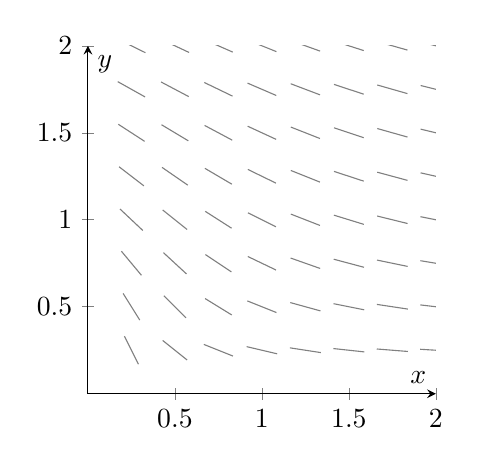
\begin{tikzpicture}\begin{axis}[width=6cm,height=6cm,axis lines=middle,xmin=0,xmax=2,ymin=0,ymax=2,xlabel=$x$,ylabel=$y$]
\draw[gray] (axis cs:0.20975,0.33050)--(axis cs:0.29025,0.16950);
\draw[gray] (axis cs:0.20230,0.57632)--(axis cs:0.29770,0.42368);
\draw[gray] (axis cs:0.19238,0.81914)--(axis cs:0.30762,0.68086);
\draw[gray] (axis cs:0.18446,1.06168)--(axis cs:0.31554,0.93832);
\draw[gray] (axis cs:0.17866,1.30487)--(axis cs:0.32134,1.19513);
\draw[gray] (axis cs:0.17449,1.54898)--(axis cs:0.32551,1.45102);
\draw[gray] (axis cs:0.17147,1.79397)--(axis cs:0.32853,1.70603);
\draw[gray] (axis cs:0.16925,2.03975)--(axis cs:0.33075,1.96025);
\draw[gray] (axis cs:0.42972,0.30622)--(axis cs:0.57028,0.19378);
\draw[gray] (axis cs:0.43636,0.56364)--(axis cs:0.56364,0.43636);
\draw[gray] (axis cs:0.43387,0.81105)--(axis cs:0.56613,0.68895);
\draw[gray] (axis cs:0.42972,1.05622)--(axis cs:0.57028,0.94378);
\draw[gray] (axis cs:0.42591,1.30110)--(axis cs:0.57409,1.19890);
\draw[gray] (axis cs:0.42283,1.54630)--(axis cs:0.57717,1.45370);
\draw[gray] (axis cs:0.42042,1.79204)--(axis cs:0.57958,1.70796);
\draw[gray] (axis cs:0.41857,2.03832)--(axis cs:0.58143,1.96168);
\draw[gray] (axis cs:0.66644,0.28343)--(axis cs:0.83356,0.21657);
\draw[gray] (axis cs:0.67335,0.54717)--(axis cs:0.82665,0.45283);
\draw[gray] (axis cs:0.67512,0.79992)--(axis cs:0.82488,0.70008);
\draw[gray] (axis cs:0.67420,1.04851)--(axis cs:0.82580,0.95149);
\draw[gray] (axis cs:0.67243,1.29563)--(axis cs:0.82757,1.20437);
\draw[gray] (axis cs:0.67059,1.54235)--(axis cs:0.82941,1.45765);
\draw[gray] (axis cs:0.66895,1.78913)--(axis cs:0.83105,1.71087);
\draw[gray] (axis cs:0.66757,2.03613)--(axis cs:0.83243,1.96387);
\draw[gray] (axis cs:0.91239,0.27061)--(axis cs:1.08761,0.22939);
\draw[gray] (axis cs:0.91644,0.53343)--(axis cs:1.08356,0.46657);
\draw[gray] (axis cs:0.91886,0.78895)--(axis cs:1.08114,0.71105);
\draw[gray] (axis cs:0.91950,1.04025)--(axis cs:1.08050,0.95975);
\draw[gray] (axis cs:0.91911,1.28946)--(axis cs:1.08089,1.21054);
\draw[gray] (axis cs:0.91828,1.53772)--(axis cs:1.08172,1.46228);
\draw[gray] (axis cs:0.91734,1.78561)--(axis cs:1.08266,1.71439);
\draw[gray] (axis cs:0.91644,2.03343)--(axis cs:1.08356,1.96657);
\draw[gray] (axis cs:1.16105,0.26369)--(axis cs:1.33895,0.23631);
\draw[gray] (axis cs:1.16324,0.52393)--(axis cs:1.33676,0.47607);
\draw[gray] (axis cs:1.16513,0.77995)--(axis cs:1.33487,0.72005);
\draw[gray] (axis cs:1.16616,1.03272)--(axis cs:1.33384,0.96728);
\draw[gray] (axis cs:1.16644,1.28343)--(axis cs:1.33356,1.21657);
\draw[gray] (axis cs:1.16625,1.53295)--(axis cs:1.33375,1.46705);
\draw[gray] (axis cs:1.16582,1.78185)--(axis cs:1.33418,1.71815);
\draw[gray] (axis cs:1.16531,2.03045)--(axis cs:1.33469,1.96955);
\draw[gray] (axis cs:1.41052,0.25967)--(axis cs:1.58948,0.24033);
\draw[gray] (axis cs:1.41175,0.51765)--(axis cs:1.58825,0.48235);
\draw[gray] (axis cs:1.41304,0.77319)--(axis cs:1.58696,0.72681);
\draw[gray] (axis cs:1.41398,1.02647)--(axis cs:1.58602,0.97353);
\draw[gray] (axis cs:1.41448,1.27804)--(axis cs:1.58552,1.22196);
\draw[gray] (axis cs:1.41462,1.52846)--(axis cs:1.58538,1.47154);
\draw[gray] (axis cs:1.41452,1.77816)--(axis cs:1.58548,1.72184);
\draw[gray] (axis cs:1.41428,2.02743)--(axis cs:1.58572,1.97257);
\draw[gray] (axis cs:1.66029,0.25718)--(axis cs:1.83971,0.24282);
\draw[gray] (axis cs:1.66101,0.51343)--(axis cs:1.83899,0.48657);
\draw[gray] (axis cs:1.66187,0.76823)--(axis cs:1.83813,0.73177);
\draw[gray] (axis cs:1.66261,1.02151)--(axis cs:1.83739,0.97849);
\draw[gray] (axis cs:1.66312,1.27348)--(axis cs:1.83688,1.22652);
\draw[gray] (axis cs:1.66339,1.52446)--(axis cs:1.83661,1.47554);
\draw[gray] (axis cs:1.66346,1.77472)--(axis cs:1.83654,1.72528);
\draw[gray] (axis cs:1.66341,2.02452)--(axis cs:1.83659,1.97548);
\draw[gray] (axis cs:1.91017,0.25553)--(axis cs:2.08983,0.24447);
\draw[gray] (axis cs:1.91062,0.51052)--(axis cs:2.08938,0.48948);
\draw[gray] (axis cs:1.91119,0.76460)--(axis cs:2.08881,0.73540);
\draw[gray] (axis cs:1.91175,1.01765)--(axis cs:2.08825,0.98235);
\draw[gray] (axis cs:1.91219,1.26973)--(axis cs:2.08781,1.23027);
\draw[gray] (axis cs:1.91249,1.52100)--(axis cs:2.08751,1.47900);
\draw[gray] (axis cs:1.91264,1.77165)--(axis cs:2.08736,1.72835);
\draw[gray] (axis cs:1.91269,2.02183)--(axis cs:2.08731,1.97817);
\end{axis}\end{tikzpicture}\end{center}
\end{solution}
\begin{exercise}\label{cw:bank-1C-3}
原题1C-3. 设 $y'=x-y$, $y(0)=1$.
\begin{enumerate}[label=\alph*)]
\item 用步长 $h=0.1$ 的 Euler 法列表估计 $y(0.1),y(0.2),y(0.3)$. 对 $y(0.3)$ 的估计偏高还是偏低? 为什么?
\item 用相同步长的改进 Euler 法(Heun 法)估计 $y(0.1)$, 说明它是否朝正确方向修正了(a)的值.
\end{enumerate}
\end{exercise}
\begin{solution}
官方答案译审. (a) $y_{j+1}=y_j+0.1(x_j-y_j)$, 得
\begin{center}\begin{tabular}{c|rrrr}$x_j$&0&0.1&0.2&0.3\\\hline$y_j$&1&0.9&0.82&0.758\end{tabular}\end{center}
精确解 $y=2e^{-x}+x-1$ 有 $y''=2e^{-x}>0$, 切线步骤位于曲线下方, 因而估计偏低. (b) 预测值为 $0.9$, 两端斜率为 $-1,-0.8$, 所以校正值 $1+0.1(-1-0.8)/2=0.91$. 精确值 $0.909674\ldots$, 修正方向向上是正确的.
\end{solution}
\begin{exercise}\label{cw:bank-1C-4}
原题1C-4. 对 $y'=x+y^2$, $y(0)=1$, 用步长 $0.1$ 的 Euler 法列表估计 $y(0.1),y(0.2),y(0.3)$. 最后的估计偏高还是偏低?
\end{exercise}
\begin{solution}
官方答案译审. 用 $y_{j+1}=y_j+0.1(x_j+y_j^2)$ 得
\begin{center}\begin{tabular}{c|rrrr}$x_j$&0&0.1&0.2&0.3\\\hline$y_j$&1&1.1&1.231&1.4025361\end{tabular}\end{center}
在此区间 $y,y'>0$, $y''=1+2yy'>0$. 每步的切线低于真曲线, 而右端对正 $y$ 单调递增, 低估会沿步骤传播, 所以最后偏低.
\end{solution}
\begin{exercise}\label{cw:bank-1C-5}
原题1C-5. 对 $y'=x-y$, $y(0)=1$, 证明 Euler 法以 $h=1/n$ 计算的 $y(1)$ 随 $n\to\infty$ 收敛到精确值. 先用归纳法证明第 $j$ 步值为 $y_j=2(1-h)^j-1+jh$. 精确解为 $y=2e^{-x}+x-1$.
\end{exercise}
\begin{solution}
官方答案译审. $j=0$ 时公式给 $1$. 若第 $j$ 步成立, 则
\[
 y_{j+1}=(1-h)y_j+jh^2=2(1-h)^{j+1}-1+(j+1)h.
\]
于是 $j=n$, $h=1/n$ 时 $y_n=2(1-1/n)^n\to2/e$, 等于精确解的 $y(1)$.
\end{solution}
\begin{exercise}\label{cw:bank-1C-6}
原题1C-6. 对 $y'=f(x)$, $y(0)=y_0$, 用四阶 Runge--Kutta 法进行 $n$ 步计算 $y(2nh)$, 每步长度为 $2h$. 精确值为 $y_0+\int_0^{2nh}f(x)dx$. 证明数值结果等于以间距 $h$ 用复合 Simpson 法计算该积分所得的值.
\end{exercise}
\begin{solution}
官方答案译审. 在 $x_j=2jh$ 的一步, 四个斜率是 $f(x_j),f(x_j+h),f(x_j+h),f(x_j+2h)$, 因而增量为 $h[f(x_j)+4f(x_j+h)+f(x_j+2h)]/3$. 对 $j=0,\ldots,n-1$ 相加正是复合 Simpson 公式. 原题的 $h$ 是半个 Runge--Kutta 步长.
\end{solution}
\begin{exercise}\label{cw:bank-1C-7}
原题1C-7. 为保证 $a(x)y'+b(x)y=c(x)$, $y(x_0)=y_0$ 在 $[x_0-h,x_0+h]$ 上有唯一解, 存在唯一性定理要求 $a,b,c$ 满足什么条件?
\end{exercise}
\begin{solution}
官方答案译审. 一个常用充分条件是 $a,b,c$ 在 $x_0$ 附近连续且 $a(x_0)\ne0$. 缩小区间使 $a\ne0$, 标准化后的 $y'=-(b/a)y+c/a$ 及其对 $y$ 的偏导 $-b/a$ 连续, 所以存在唯一解. 更直接的条件是 $b/a,c/a$ 在该区间连续, 不必要求三个分子分母分别连续.
\end{solution}
\originalsection{1D: 几何与物理应用}
\begin{exercise}\label{cw:bank-1D-1}
原题1D-1. 将几何条件写成微分方程, 求所有满足条件的曲线 $y=y(x)$:
\begin{enumerate}[label=\alph*)]
\item 每条切线在第一象限内的线段, 被切点平分.
\item 每条法线从曲线到 $x$ 轴之间的线段长度恒为1.
\item 每条法线从曲线到 $x$ 轴之间的线段, 被 $y$ 轴平分.
\item 固定 $a$, 曲线在 $a$ 与 $x$ 之间的有向面积与 $y(x)-y(a)$ 成正比.
\end{enumerate}
\end{exercise}
\begin{solution}
官方答案译审. (a) 切点 $(x,y)$ 是两轴截点 $(2x,0),(0,2y)$ 的中点, 故 $y'=-y/x$, 得 $xy=C$, 在第一象限取 $C>0$. (b) 法线斜率为 $-1/y'$, 它与 $x$ 轴的交点为 $(x+yy',0)$, 故长度平方 $y^2(1+(y')^2)=1$. 分离得 $(x-C)^2+y^2=1$, 取可作为函数的圆弧; 另有水平线 $y=\pm1$. (c) 平分条件给法线另一端横坐标 $-x$, 故法线斜率 $y/(2x)=-1/y'$, 得 $yy'=-2x$, 所以 $x^2+y^2/2=C$. (d) 写成 $\int_a^x y(t)dt=k[y(x)-y(a)]$, 对 $x$ 求导得 $y=ky'$. $k\ne0$ 时 $y=Ce^{x/k}$; $k=0$ 只给零函数.
\end{solution}
\begin{exercise}\label{cw:bank-1D-2}
原题1D-2. 对每个曲线族: (i) 求以它为积分曲线的微分方程; (ii) 求正交轨线; (iii) 同图画出原族和正交族.
\begin{enumerate}[label=\alph*)]
\item $y$ 轴截距为斜率两倍的直线.
\item 指数曲线 $y=ce^x$.
\item 双曲线 $x^2-y^2=c$.
\item 圆心在 $y$ 轴且与 $x$ 轴相切的圆.
\end{enumerate}
\end{exercise}
\begin{solution}
官方答案译审. 正交方向将有限非零斜率 $m$ 换成 $-1/m$, 竖直/水平处用隐式曲线理解.
(a) $y=m(x+2)$, 原方程 $y'=y/(x+2)$; 正交式 $yy'=-(x+2)$, 得 $(x+2)^2+y^2=C$. (b) 原方程 $y'=y$, 正交式 $yy'=-1$, 得 $y^2+2x=C$. (c) 原式 $yy'=x$, 正交式 $y'=-y/x$, 得 $xy=C$. (d) 原族 $x^2+y^2=2ay$, 消去 $a$ 得 $y'=2xy/(x^2-y^2)$. 正交式 $y'=(y^2-x^2)/(2xy)$. 令 $y=xz$ 积分, 得 $x^2+y^2=Cx$: 圆心在 $x$ 轴并与 $y$ 轴相切的圆.
\begin{center}\begin{tikzpicture}
\begin{axis}[width=6.5cm,height=6.5cm,axis lines=middle,xmin=-4,xmax=1,ymin=-2,ymax=2,title={(a)},clip=true]
\addplot[main,domain=-4:1] {-1*(x+2)};
\addplot[main,domain=-4:1] {-0.5*(x+2)};
\addplot[main,domain=-4:1] {0.5*(x+2)};
\addplot[main,domain=-4:1] {1*(x+2)};
\addplot[black,dashed,domain=0:360,samples=90] ({-2+0.5*cos(x)},{0.5*sin(x)});
\addplot[black,dashed,domain=0:360,samples=90] ({-2+1*cos(x)},{1*sin(x)});
\addplot[black,dashed,domain=0:360,samples=90] ({-2+1.5*cos(x)},{1.5*sin(x)});
\end{axis}\end{tikzpicture}\quad
\begin{tikzpicture}\begin{axis}[width=6.5cm,height=6.5cm,axis lines=middle,xmin=-2,xmax=2,ymin=-2,ymax=2,title={(b)},clip=true]
\addplot[main,domain=-2:2] {-1*exp(x)};
\addplot[main,domain=-2:2] {-0.5*exp(x)};
\addplot[main,domain=-2:2] {0.5*exp(x)};
\addplot[main,domain=-2:2] {1*exp(x)};
\addplot[black,dashed,domain=-2:2,samples=80] ({(-1-x*x)/2},{x});
\addplot[black,dashed,domain=-2:2,samples=80] ({(0-x*x)/2},{x});
\addplot[black,dashed,domain=-2:2,samples=80] ({(1-x*x)/2},{x});
\addplot[black,dashed,domain=-2:2,samples=80] ({(2-x*x)/2},{x});
\end{axis}\end{tikzpicture}
\begin{tikzpicture}\begin{axis}[width=6.5cm,height=6.5cm,axis lines=middle,xmin=-2,xmax=2,ymin=-2,ymax=2,title={(c)},clip=true]
\addplot[main,domain=-2:2] ({0.5*cosh(x)},{0.5*sinh(x)});\addplot[main,domain=-2:2] ({-0.5*cosh(x)},{0.5*sinh(x)});\addplot[main,domain=-2:2] ({0.5*sinh(x)},{0.5*cosh(x)});\addplot[main,domain=-2:2] ({0.5*sinh(x)},{-0.5*cosh(x)});
\addplot[main,domain=-2:2] ({1*cosh(x)},{1*sinh(x)});\addplot[main,domain=-2:2] ({-1*cosh(x)},{1*sinh(x)});\addplot[main,domain=-2:2] ({1*sinh(x)},{1*cosh(x)});\addplot[main,domain=-2:2] ({1*sinh(x)},{-1*cosh(x)});
\addplot[black,dashed,domain=-2:-0.1] {-1/x};\addplot[black,dashed,domain=0.1:2] {-1/x};
\addplot[black,dashed,domain=-2:-0.1] {-0.5/x};\addplot[black,dashed,domain=0.1:2] {-0.5/x};
\addplot[black,dashed,domain=-2:-0.1] {0.5/x};\addplot[black,dashed,domain=0.1:2] {0.5/x};
\addplot[black,dashed,domain=-2:-0.1] {1/x};\addplot[black,dashed,domain=0.1:2] {1/x};
\end{axis}\end{tikzpicture}\quad
\begin{tikzpicture}\begin{axis}[width=6.5cm,height=6.5cm,axis lines=middle,xmin=-2,xmax=2,ymin=-2,ymax=2,title={(d)},clip=true]
\addplot[main,domain=0:360,samples=90] ({abs(-1)*cos(x)},{-1+abs(-1)*sin(x)});\addplot[black,dashed,domain=0:360,samples=90] ({-1+abs(-1)*cos(x)},{abs(-1)*sin(x)});
\addplot[main,domain=0:360,samples=90] ({abs(-0.5)*cos(x)},{-0.5+abs(-0.5)*sin(x)});\addplot[black,dashed,domain=0:360,samples=90] ({-0.5+abs(-0.5)*cos(x)},{abs(-0.5)*sin(x)});
\addplot[main,domain=0:360,samples=90] ({abs(0.5)*cos(x)},{0.5+abs(0.5)*sin(x)});\addplot[black,dashed,domain=0:360,samples=90] ({0.5+abs(0.5)*cos(x)},{abs(0.5)*sin(x)});
\addplot[main,domain=0:360,samples=90] ({abs(1)*cos(x)},{1+abs(1)*sin(x)});\addplot[black,dashed,domain=0:360,samples=90] ({1+abs(1)*cos(x)},{abs(1)*sin(x)});
\end{axis}\end{tikzpicture}\end{center}
实线表示原族, 虚线表示正交族.
\end{solution}
\begin{exercise}\label{cw:bank-1D-3}
原题1D-3. 容器有 $V$ 升盐水, 初浓度 $c_0$ 克/升. 浓度 $c_1$ 的盐水以 $k$ 升/分流入并立即均匀混合, 混合液以同速流出. 设盐量 $x(t)$, 浓度 $c=x/V$.
\begin{enumerate}[label=\alph*)]
\item 建立 $x$ 的方程及初值.
\item 流入纯水时求解, 记 $a=k/V$.
\item $c_1$ 恒定时求 $c(t)$ 及其极限, 解释极限.
\item 改设 $c_1(t)=c_0e^{-\alpha t}$, $\alpha>0$, $a\ne\alpha$. 求 $c(t)$, 并令 $\alpha=0$ 与(c)比较.
\end{enumerate}
\end{exercise}
\begin{solution}
官方答案译审. (a) 流入盐速率 $kc_1$, 流出速率 $kx/V$, 故 $x'+ax=kc_1$, $x(0)=Vc_0$. (b) $c=c_0e^{-at}$. (c) 积分因子给 $c=c_1+(c_0-c_1)e^{-at}\to c_1$: 长期换水使原盐水被输入盐水替换. (d) $c'+ac=ac_0e^{-\alpha t}$, 故
\[
 c(t)=\frac{ac_0}{a-\alpha}e^{-\alpha t}-\frac{\alpha c_0}{a-\alpha}e^{-at}.
\]
$\alpha=0$ 给 $c=c_0$, 与(c)取 $c_1=c_0$ 一致. 若补取 $a=\alpha$, 则 $c=c_0(1+at)e^{-at}$.
\end{solution}
\begin{exercise}\label{cw:bank-1D-4}
原题1D-4. 放射性物质 $A$ 衰变为 $B$, $B$ 再衰变为 $C$.
\begin{enumerate}[label=\alph*)]
\item 衰变常数分别为 $\lambda_1,\lambda_2$ (定义为 $\ln2$/半衰期), 初始量分别为 $A_0,B_0$. 建立并解 $B(t)$ 的方程, 假设 $\lambda_1\ne\lambda_2$.
\item 设 $\lambda_1=1,\lambda_2=2$, 求 $B$ 达到最大值的时间.
\end{enumerate}
\end{exercise}
\begin{solution}
官方答案译审并补核边界. (a) $A=A_0e^{-\lambda_1t}$, $B'+\lambda_2B=\lambda_1A_0e^{-\lambda_1t}$, $B(0)=B_0$, 所以
\[
 B=\frac{\lambda_1A_0}{\lambda_2-\lambda_1}e^{-\lambda_1t}+\left(B_0-\frac{\lambda_1A_0}{\lambda_2-\lambda_1}\right)e^{-\lambda_2t}.
\]
(b) $B=A_0e^{-t}+(B_0-A_0)e^{-2t}$. 对非负初量, 若 $A_0>2B_0$, 导数零点为 $t_* =\ln[2(A_0-B_0)/A_0]>0$, 导数先正后负. 若 $A_0\le2B_0$, $B$ 从 $t=0$ 起递减或立即开始递减, 最大值在 $t=0$. $A_0=B_0=0$ 时处处取最大值零.
\end{solution}
\begin{exercise}\label{cw:bank-1D-5}
原题1D-5. Newton 冷却律说温度变化率与物体和环境的温差成正比. 一锅沸水在 $t=0$ 离火, 5分钟后为 $80^\circ\mathrm C$, 室温 $20^\circ\mathrm C$. 建模并求何时降到 $60^\circ\mathrm C$.
\end{exercise}
\begin{solution}
官方答案译审. $T'=-k(T-20)$, $T(0)=100$, 故 $T=20+80e^{-kt}$. 由 $T(5)=80$ 得 $e^{-5k}=3/4$, $k=\ln(4/3)/5$. 降到60时 $e^{-kt}=1/2$, 所以 $t=5\ln2/\ln(4/3)\approx12.05$ 分钟.
\end{solution}
\begin{exercise}\label{cw:bank-1D-6}
原题1D-6. 质量 $m$ 的物体在重力下穿过空气下落, 重力加速度为 $g$. 求速度 $v(t)$ 与终端速度, 分别假设 (a) 阻力为 $kv$ (小速度); (b) 阻力为 $kv^2$ (高速度). (b)可记 $a=\sqrt{gm/k}$.
\end{exercise}
\begin{solution}
官方答案以静止释放为初值; 原题未指定初速, 此处同时给初速参数. 取向下为正. (a) $mv'=mg-kv$, 故 $v=mg/k+(v_0-mg/k)e^{-kt/m}$, 终端速度 $mg/k$. (b) 在向下运动阶段 $mv'=mg-kv^2$. 对 $0\le v_0<a$, 分离得
\[
 v=a\tanh\left(\frac{g}{a}t+\operatorname{arctanh}(v_0/a)\right).
\]
$v_0=0$ 时为 $a\tanh(gt/a)$, 终端速度 $a$. $v_0=a$ 为常数解, $v_0>a$ 时用 $a\coth(gt/a+\operatorname{arccoth}(v_0/a))$, 极限仍为 $a$.
\end{solution}
\begin{exercise}\label{cw:bank-1D-7}
原题1D-7. 受载缆索悬于两个支点, 最低点为 $Q$. 弧段 $QP$ 受其总载荷 $W$、$Q$ 处恒定水平张力 $T_Q$、$P$ 处张力 $T$. $s$ 为 $QP$ 弧长, $x,y$ 是以 $Q$ 附近水平、竖直方向为坐标的曲线参数.
\begin{enumerate}[label=\alph*)]
\item 证明 $dx/T_Q=dy/W=ds/T$.
\item 自重均匀时证明 (i) $y''=k\sqrt{1+(y')^2}$; (ii) $y=\sqrt{s^2+c^2}+c_1$.
\item 缆索自重可忽略、载荷按水平距离均匀分布时, 求悬索桥缆索 $y(x)$.
\item 缆索自重可忽略, 悬挂等间距且密集的竖杆, 杆底端在同一水平线. 以此线为 $x$ 轴, 证明 Marseille 幕帘曲线满足 $y''=k^2y$.
\end{enumerate}
\end{exercise}
\begin{solution}
官方答案译审. (a) 切线角 $\phi$ 满足 $T\cos\phi=T_Q$, $T\sin\phi=W$, 而 $\cos\phi=dx/ds$, $\sin\phi=dy/ds$, 即所求比例. (b) 每单位弧长重量为 $\rho$, 则 $W=\rho s$, $y'=W/T_Q=ks$, $k=\rho/T_Q$. 求导给(i). 又 $ds/dy=T/W=\sqrt{T_Q^2+\rho^2s^2}/(\rho s)$, 积分得 $y=\sqrt{s^2+(T_Q/\rho)^2}+c_1$. 相应 $y(x)=k^{-1}\cosh(k(x-x_Q))+C$. (c) 水平载荷密度 $\lambda$ 时 $W=\lambda(x-x_Q)$, 故 $y'=\lambda(x-x_Q)/T_Q$, $y=\lambda(x-x_Q)^2/(2T_Q)+C$. (d) 竖杆重量与长度 $y$ 成正比, 密集极限的水平载荷密度为 $\lambda y$. 因而 $W'=\lambda y$, $y''=W'/T_Q=(\lambda/T_Q)y=k^2y$. 最低点对称的解为 $C\cosh(k(x-x_Q))$.
\end{solution}
\originalsection{1E: 一阶自治方程}
\begin{exercise}\label{cw:bank-1E-1}
原题1E-1. 对 $dx/dt=f(x)$: (i) 在水平 $x$ 轴标出平衡点和运动箭头, 判定稳定、不稳定或半稳定, 并用虚线画 $f(x)$ 说明符号来源; (ii) 在 $tx$ 平面画典型解, 包括常数解和非常数解的渐近行为.
\begin{enumerate}[label=\alph*)]
\item $x'=x^2+2x$. \item $x'=-(x-1)^2$. \item $x'=2x-x^2$. \item $x'=(2-x)^3$.
\end{enumerate}
\end{exercise}
\begin{solution}
官方答案译审. (a) 符号在 $(-\infty,-2),(-2,0),(0,\infty)$ 为 $+,-,+$, 所以 $-2$ 稳定, $0$ 不稳定. (b) 除 $1$ 外均为负, $1$ 从右吸引、从左排斥, 半稳定. (c) 符号在 $(-\infty,0),(0,2),(2,\infty)$ 为 $-,+,-$, 所以 $0$ 不稳定, $2$ 稳定. (d) $x<2$ 时正、$x>2$ 时负, $2$ 稳定. 典型解可由分离求得: (a) $x=2Ce^{2t}/(1-Ce^{2t})$; (b) $x=1+1/(t+C)$; (c) $x=2/(1+Ce^{-2t})$; (d) $x=2\pm(2t+C)^{-1/2}$. 各式只取其最大有定义区间, 并补回常数解. 发散分支可能在有限时间爆破, 不能把所有解都画成全时间存在.
\begin{center}
\begin{tikzpicture}\begin{axis}[width=6cm,height=4.2cm,axis lines=middle,xmin=-3,xmax=1,ymin=-3,ymax=3,xlabel=$x$,ylabel=$f(x)$,title={(a)},clip=true]\addplot[dashed,domain=-3:1,samples=70] {x*x+2*x};
\draw[-{Stealth},main,thick] (axis cs:-2.70,0)--(axis cs:-2.45,0);
\draw[-{Stealth},main,thick] (axis cs:-1.00,0)--(axis cs:-1.25,0);
\draw[-{Stealth},main,thick] (axis cs:0.70,0)--(axis cs:0.95,0);
\fill[main] (axis cs:-2,0) circle (2pt);
\fill[main] (axis cs:0,0) circle (2pt);
\end{axis}\end{tikzpicture}\quad\begin{tikzpicture}\begin{axis}[width=6cm,height=4.2cm,axis lines=middle,xmin=0,xmax=2,ymin=-3,ymax=4,xlabel=$t$,ylabel=$x$,clip=true]
\addplot[main,domain=0:2,samples=80] {-2};
\addplot[main,domain=0:2,samples=80] {0};
\addplot[main,domain=0:2,samples=80] {2*(-0.3)*exp(2*x)/(1+0.3*exp(2*x))};
\addplot[main,domain=0:1.49,samples=80] {2*0.05*exp(2*x)/(1-0.05*exp(2*x))};
\addplot[main,domain=0:2,samples=80] {4*exp(2*x)/(1-2*exp(2*x))};
\end{axis}\end{tikzpicture}
\begin{tikzpicture}\begin{axis}[width=6cm,height=4.2cm,axis lines=middle,xmin=-1,xmax=3,ymin=-3,ymax=3,xlabel=$x$,ylabel=$f(x)$,title={(b)},clip=true]\addplot[dashed,domain=-1:3,samples=70] {-(x-1)^2};
\draw[-{Stealth},main,thick] (axis cs:-0.70,0)--(axis cs:-0.95,0);
\draw[-{Stealth},main,thick] (axis cs:0.30,0)--(axis cs:0.05,0);
\draw[-{Stealth},main,thick] (axis cs:2.70,0)--(axis cs:2.45,0);
\fill[main] (axis cs:1,0) circle (2pt);
\end{axis}\end{tikzpicture}\quad\begin{tikzpicture}\begin{axis}[width=6cm,height=4.2cm,axis lines=middle,xmin=0,xmax=2,ymin=-3,ymax=4,xlabel=$t$,ylabel=$x$,clip=true]
\addplot[main,domain=0:2,samples=80] {1};
\addplot[main,domain=0:2,samples=80] {1+1/(x+1)};
\addplot[main,domain=0:2,samples=80] {1+1/(x-3)};
\end{axis}\end{tikzpicture}
\begin{tikzpicture}\begin{axis}[width=6cm,height=4.2cm,axis lines=middle,xmin=-1,xmax=3,ymin=-3,ymax=3,xlabel=$x$,ylabel=$f(x)$,title={(c)},clip=true]\addplot[dashed,domain=-1:3,samples=70] {2*x-x*x};
\draw[-{Stealth},main,thick] (axis cs:-0.70,0)--(axis cs:-0.95,0);
\draw[-{Stealth},main,thick] (axis cs:1.00,0)--(axis cs:1.25,0);
\draw[-{Stealth},main,thick] (axis cs:2.70,0)--(axis cs:2.45,0);
\fill[main] (axis cs:0,0) circle (2pt);
\fill[main] (axis cs:2,0) circle (2pt);
\end{axis}\end{tikzpicture}\quad\begin{tikzpicture}\begin{axis}[width=6cm,height=4.2cm,axis lines=middle,xmin=0,xmax=2,ymin=-3,ymax=4,xlabel=$t$,ylabel=$x$,clip=true]
\addplot[main,domain=0:2,samples=80] {0};
\addplot[main,domain=0:2,samples=80] {2};
\addplot[main,domain=0:2,samples=80] {2/(1+3*exp(-2*x))};
\addplot[main,domain=0:2,samples=80] {2/(1-0.5*exp(-2*x))};
\addplot[main,domain=0:0.545,samples=100] {2/(1-3*exp(-2*x))};
\end{axis}\end{tikzpicture}
\begin{tikzpicture}\begin{axis}[width=6cm,height=4.2cm,axis lines=middle,xmin=0,xmax=4,ymin=-3,ymax=3,xlabel=$x$,ylabel=$f(x)$,title={(d)},clip=true]\addplot[dashed,domain=0:4,samples=70] {(2-x)^3};
\draw[-{Stealth},main,thick] (axis cs:0.30,0)--(axis cs:0.55,0);
\draw[-{Stealth},main,thick] (axis cs:1.50,0)--(axis cs:1.75,0);
\draw[-{Stealth},main,thick] (axis cs:3.70,0)--(axis cs:3.45,0);
\fill[main] (axis cs:2,0) circle (2pt);
\end{axis}\end{tikzpicture}\quad\begin{tikzpicture}\begin{axis}[width=6cm,height=4.2cm,axis lines=middle,xmin=0,xmax=2,ymin=-3,ymax=4,xlabel=$t$,ylabel=$x$,clip=true]
\addplot[main,domain=0:2,samples=80] {2};
\addplot[main,domain=0:2,samples=80] {2+1/sqrt(2*x+0.4)};
\addplot[main,domain=0:2,samples=80] {2-1/sqrt(2*x+0.4)};
\end{axis}\end{tikzpicture}
\end{center}\end{solution}
\originalchapter{题库二: 高阶线性微分方程}
\originalsection{2A: 二阶线性方程的一般性质}
\begin{exercise}\label{cw:bank-2A-1}
原题2A-1. 设 $L=D^2+p(x)D+q(x)$, 方程为 $Ly=r(x)$. (a) 对任意二次可微函数 $u_1,u_2$ 和常数 $c$, 验证 $L(u_1+u_2)=Lu_1+Lu_2$, $L(cu_1)=cLu_1$. (b) 若 $y_p$ 是一个特解, 证明全部解恰为 $y=y_c+y_p$, 其中 $Ly_c=0$.
\end{exercise}
\begin{solution}
官方答案译审. (a) 求导、乘以固定函数及相加都保持加法和数乘, 逐项展开即得两式. (b) 若 $Ly_c=0$, 则 $L(y_c+y_p)=r$; 反之任意解 $y$ 满足 $L(y-y_p)=r-r=0$, 所以 $y-y_p$ 是齐次解.
\end{solution}
\begin{exercise}\label{cw:bank-2A-2}
原题2A-2. (a) 消去常数, 求通解为 $y=c_1e^x+c_2e^{2x}$ 的二阶齐次线性方程. (b) 验证任意初值 $y(x_0)=y_0$, $y\prime(x_0)=v_0$ 都能实现.
\end{exercise}
\begin{solution}
官方答案译审. (a) $y\prime-y=c_2e^{2x}$, 再求导得 $y\prime\prime-3y\prime+2y=0$. (b) 初值系数矩阵行列式 $e^{3x_0}\ne0$, 故有唯一 $c_1,c_2$; 具体 $c_2=e^{-2x_0}(v_0-y_0)$, $c_1=e^{-x_0}(2y_0-v_0)$.
\end{solution}
\begin{exercise}\label{cw:bank-2A-3}
原题2A-3. (a) 消去常数, 求通解为 $y=c_1x+c_2x^2$ 的二阶齐次线性方程. (b) 证明它没有满足 $y(0)=1,y\prime(0)=1$ 的解. (c) 为什么不违背二阶线性方程存在定理?
\end{exercise}
\begin{solution}
官方答案译审. (a) $y\prime\prime=2c_2$, 消去得 $x^2y\prime\prime-2xy\prime+2y=0$. (b) 在原方程 $x=0$ 处直接得到 $2y(0)=0$, 与初值矛盾. (c) 标准式系数 $-2/x,2/x^2$ 在0不连续, 不满足定理条件.
\end{solution}
\begin{exercise}\label{cw:bank-2A-4}
原题2A-4. 考虑 $y\prime\prime+p(x)y\prime+q(x)y=0$. (a) 若 $p,q$ 在全实轴连续, 证明图形在某处与 $x$ 轴相切的解恒为零. (b) 写出以 $x^2$ 为解的上述形式方程, 说明它为什么不违背(a).
\end{exercise}
\begin{solution}
官方答案译审. (a) 相切点 $x_0$ 给 $y(x_0)=y\prime(x_0)=0$. 零解有相同初值, 全实轴上的唯一性给 $y\equiv0$. (b) $xy\prime\prime-y\prime=0$, 即 $y\prime\prime-y\prime/x=0$ ($x\ne0$); 标准式系数在0不连续.
\end{solution}
\begin{exercise}\label{cw:bank-2A-5}
原题2A-5. 计算 Wronskian, 证明下列函数对线性无关: (a) $e^{m_1x},e^{m_2x}$, $m_1\ne m_2$; (b) $e^{mx},xe^{mx}$; (b)允许 $m=0$ 吗?
\end{exercise}
\begin{solution}
官方答案译审. (a) $W=(m_2-m_1)e^{(m_1+m_2)x}\ne0$. (b) $W=e^{2mx}\ne0$, 包括 $m=0$, 此时函数对为 $1,x$.
\end{solution}
\begin{exercise}\label{cw:bank-2A-6}
原题2A-6. 设 $y_1=x^2,y_2=x|x|$, 画 $y_2$ 的图. (a) 证明 $W(y_1,y_2)\equiv0$. (b) 证明两函数在任何含0的区间 $(a,b)$ 上不线性相关, 并说明为什么不违背解函数的 Wronskian 判别定理.
\end{exercise}
\begin{solution}
官方答案译审. $y_2$ 在右半轴为 $x^2$, 左半轴为 $-x^2$, 图由这两条抛物线弧拼成. 两侧各有 $W=0$, 在0也为0. 若 $c_1y_1+c_2y_2=0$, 右侧给 $c_1+c_2=0$, 左侧给 $c_1-c_2=0$, 所以两常数都零. 判别定理要求二者是同一正则线性方程的解; $y_2$ 在0没有二阶导数, 不满足要求.\begin{center}\begin{tikzpicture}\begin{axis}[width=6cm,height=4cm,axis lines=middle,xmin=-2,xmax=2,ymin=-4,ymax=4,xlabel=$x$,ylabel=$y_2$]\addplot[main,domain=-2:0] {-x^2};\addplot[main,domain=0:2] {x^2};\end{axis}\end{tikzpicture}\end{center}
\end{solution}
\begin{exercise}\label{cw:bank-2A-7}
原题2A-7. 设 $y_1,y_2$ 是 $y\prime\prime+py\prime+qy=0$ 的解. (a) 证明 $W\prime=-pW$. (b) 推出 $p=0$ 时 $W$ 恒定. (c) 对 $y\prime\prime+k^2y=0$, $k\ne0$, 直接验证(b), 其解为 $c_1\sin kx+c_2\cos kx$.
\end{exercise}
\begin{solution}
官方答案译审. (a) 对 $W=y_1y_2\prime-y_1\prime y_2$ 求导, 得 $W\prime=y_1y_2\prime\prime-y_1\prime\prime y_2=-p(y_1y_2\prime-y_1\prime y_2)$. (b) $W\prime=0$. (c) 取两个解的系数分别为 $(a,b),(c,d)$, 直接得到 $W=k(bc-ad)$, 与 $x$ 无关.
\end{solution}
\originalsection{2B: 降阶法}
\begin{exercise}\label{cw:bank-2B-1}
原题2B-1. 已知 $y_1=e^x$ 解 $y\prime\prime-2y\prime+y=0$, 分别 (a) 令 $y_2=ue^x$ 代入; (b) 先由2A-7求 $W$ 再求 $y_2$; (c) 用公式 $y_2=y_1\int e^{-\int p dx}/y_1^2\,dx$, 求第二解. (d) 解释结果的可能差异, 写最一般的第二解.
\end{exercise}
\begin{solution}
官方答案译审. (a) 代入得 $e^xu\prime\prime=0$, 故 $y_2=(Ax+B)e^x$, $A\ne0$. (b) $W\prime=2W$ 给 $W=Ke^{2x}$, 而 $W=e^x(y_2\prime-y_2)$, 故 $(e^{-x}y_2)\prime=K$, 给同一式. (c) 被积函数为 $e^{2x}/e^{2x}=1$, 得 $xe^x$ 加常数倍 $e^x$. (d) 非零倍数及加上第一解不改变独立性, 最一般式为 $(Ax+B)e^x$, $A\ne0$.
\end{solution}
\begin{exercise}\label{cw:bank-2B-2}
原题2B-2. 证明2B-1(c)的一般降阶公式给出的 $y_2$ 与 $y_1$ 线性无关, 可计算其 Wronskian.
\end{exercise}
\begin{solution}
官方答案译审. 设 $I\prime=e^{-\int p dx}/y_1^2$, $y_2=y_1I$, 则 $W=y_1^2I\prime=e^{-\int p dx}\ne0$. 公式先在 $y_1\ne0$ 的区间使用; 第二解可按正则方程延拓.
\end{solution}
\begin{exercise}\label{cw:bank-2B-3}
原题2B-3. 已知 $y_1=x$ 解 $x^2y\prime\prime+2xy\prime-2y=0$, 用 $y_2=xu$ 降阶求第二解.
\end{exercise}
\begin{solution}
官方答案译审. 代入得 $x^3u\prime\prime+4x^2u\prime=0$, 令 $v=u\prime$, 则 $v\prime=-4v/x$, $v=Cx^{-4}$. 再积分 $u=A+Bx^{-3}$, 第二解可取 $x^{-2}$, $x\ne0$.
\end{solution}
\begin{exercise}\label{cw:bank-2B-4}
原题2B-4. 已知 $y_1=x$ 为解, 求 $(1-x^2)y\prime\prime-2xy\prime+2y=0$ 在 $(-1,1)$ 上的通解.
\end{exercise}
\begin{solution}
官方答案译审. $e^{-\int p dx}=(1-x^2)^{-1}$, 且 $1/[x^2(1-x^2)]=1/x^2+1/[2(1-x)]+1/[2(1+x)]$. 公式给第二解 $-1+\frac{x}{2}\ln\frac{1+x}{1-x}$. 因而 $y=Ax+B[1-\frac{x}{2}\ln\frac{1+x}{1-x}]$. 该式在0平滑, 可直接验证并由唯一性延拓穿过0.
\end{solution}
\originalsection{2C: 常系数二阶方程}
\begin{exercise}\label{cw:bank-2C-1}
原题2C-1. 求通解或给定初值解: (a) $y\prime\prime-3y\prime+2y=0$; (b) $y\prime\prime+2y\prime-3y=0$, $y(0)=1,y\prime(0)=-1$; (c) $y\prime\prime+2y\prime+2y=0$; (d) $y\prime\prime-2y\prime+5y=0$, $y(0)=1,y\prime(0)=-1$; (e) $y\prime\prime-4y\prime+4y=0$, $y(0)=1,y\prime(0)=1$.
\end{exercise}
\begin{solution}
官方答案译审. 特征根依次为 $(1,2),(1,-3),(-1\pm i),(1\pm2i),(2,2)$. 因而 (a) $Ae^x+Be^{2x}$; (b) 初值给 $A+B=1,A-3B=-1$, 得 $(e^x+e^{-3x})/2$; (c) $e^{-x}(A\cos x+B\sin x)$; (d) $e^x(\cos2x-\sin2x)$; (e) $(1-x)e^{2x}$.
\end{solution}
\begin{exercise}\label{cw:bank-2C-2}
原题2C-2. 用 Wronskian 证明 $e^{ax}\cos bx,e^{ax}\sin bx$ 线性无关, 并说明 $a,b$ 的限制.
\end{exercise}
\begin{solution}
官方答案译审. $W=be^{2ax}$. 所以任意实 $a$ 都可, 必须 $b\ne0$; 若 $b=0$, 第二函数恒零.
\end{solution}
\begin{exercise}\label{cw:bank-2C-3}
原题2C-3. 考虑 $y\prime\prime+cy\prime+4y=0$, $c$ 为常数. 说明哪些 $c$ 满足: (a) 存在振荡解; (b) 所有非零解为衰减振荡.
\end{exercise}
\begin{solution}
官方答案译审. 特征根 $(-c\pm\sqrt{c^2-16})/2$. (a) 需非实根, 即 $-4<c<4$. (b) 再要求实部 $-c/2<0$, 即 $0<c<4$.
\end{solution}
\begin{exercise}\label{cw:bank-2C-4}
原题2C-4. Euler 等维方程 $x^2y\prime\prime+pxy\prime+qy=0$, $p,q$ 为常数. (a) 证明 $x=e^t$ 化为常系数方程. (b) 据此解 $x^2y\prime\prime+xy\prime+y=0$.
\end{exercise}
\begin{solution}
官方答案译审. 令 $Y(t)=y(e^t)$, 则 $xy\prime=\dot Y$, $x^2y\prime\prime=\ddot Y-\dot Y$, 所以 $\ddot Y+(p-1)\dot Y+qY=0$. (b) $\ddot Y+Y=0$, 得 $y=A\cos\ln x+B\sin\ln x$, $x>0$; 在负半轴以 $\ln|x|$ 给同样公式.
\end{solution}
\begin{exercise}\label{cw:bank-2C-5}
原题2C-5. 阻尼弹簧质量系统 $mx\prime\prime+cx\prime+kx=0$ 何时临界阻尼, 即恰处于振荡与非振荡的边界?
\end{exercise}
\begin{solution}
官方答案译审. 对 $m,k>0,c\ge0$, 特征式 $mr^2+cr+k=0$ 的判别式必须为零, 即 $c^2=4mk$, $c=2\sqrt{mk}$.
\end{solution}
\begin{exercise}\label{cw:bank-2C-6}
原题2C-6. 摆长 $L$, 质量 $m$, 切向阻力为 $mc\,d\alpha/dt$. 说明小摆角 $\alpha$ 近似服从常系数二阶方程. 无阻尼 $c=0$ 时用 $L,m,g$ 表示周期.
\end{exercise}
\begin{solution}
官方答案译审. 切向 Newton 方程为 $mL\alpha\prime\prime=-mg\sin\alpha-mc\alpha\prime$, 故 $\alpha\prime\prime+(c/L)\alpha\prime+(g/L)\alpha=0$ (用 $\sin\alpha\approx\alpha$). 无阻尼时角频率 $\sqrt{g/L}$, 周期 $2\pi\sqrt{L/g}$, 不依赖质量.
\end{solution}
\begin{exercise}\label{cw:bank-2C-7}
原题2C-7. 只写待定系数法所需的特解试探形式: (a) $y\prime\prime+2y\prime+2y=x+e^x$; (b) $y\prime\prime-4y\prime=\cos2x$; (c) $y\prime\prime+4y=3\cos2x$; (d) $y\prime\prime-2y\prime+y=3e^x$; (e) $y\prime\prime-3y\prime+2y=e^{-x}+3e^{2x}$; (f) $y\prime\prime-6y\prime+9y=2xe^{3x}$.
\end{exercise}
\begin{solution}
官方答案译审. 依次取 (a) $Ax+B+Ce^x$; (b) $A\cos2x+B\sin2x$; (c) $x(A\cos2x+B\sin2x)$; (d) $Ax^2e^x$; (e) $Ae^{-x}+Bxe^{2x}$; (f) $x^2(Ax+B)e^{3x}$. 每个共振项乘 $x$ 的次数等于对应特征根的重数.
\end{solution}
\begin{exercise}\label{cw:bank-2C-8}
原题2C-8. 求通解或初值解: (a) $y\prime\prime-6y\prime+5y=e^x$; (b) $y\prime\prime+4y=2\cos x$, $y(0)=0,y\prime(0)=1$; (c) $y\prime\prime+y\prime+y=2xe^x$; (d) $y\prime\prime-y=x^2$, $y(0)=0,y\prime(0)=-1$.
\end{exercise}
\begin{solution}
官方答案译审. (a) 特征根1,5, 试 $Axe^x$, 代入给 $-4Ae^x=e^x$, 故 $y=C_1e^x+C_2e^{5x}-xe^x/4$. (b) 特解 $2\cos x/3$, 初值得 $y=-2\cos2x/3+\sin2x/2+2\cos x/3$. (c) 试 $e^x(Ax+B)$, 移位后为 $e^x[(D^2+3D+3)(Ax+B)]$, 给 $A=2/3,B=-2/3$, 因而 $y=e^{-x/2}[C_1\cos(\sqrt3x/2)+C_2\sin(\sqrt3x/2)]+2(x-1)e^x/3$. (d) 特解 $-x^2-2$, 初值解 $y=e^x/2+3e^{-x}/2-x^2-2$.
\end{solution}
\begin{exercise}\label{cw:bank-2C-9}
原题2C-9. 对 $Ly=y\prime\prime+py\prime+qy=r$, (a) 若 $Ly_i=r_i$ ($i=1,2$), 证明 $y_1+y_2$ 是输入 $r_1+r_2$ 的特解. (b) 据此求 $y\prime\prime+2y\prime+2y=2x+\cos x$ 的特解.
\end{exercise}
\begin{solution}
官方答案译审. (a) 线性性给 $L(y_1+y_2)=r_1+r_2$. (b) 输入 $2x$ 试 $Ax+B$, 得 $A=1,B=-1$; 输入 $\cos x$ 试 $a\cos x+b\sin x$, 得 $a+2b=1,b-2a=0$, 所以 $y_p=x-1+\cos x/5+2\sin x/5$.
\end{solution}
\begin{exercise}\label{cw:bank-2C-10}
原题2C-10. 串联 RLC 电路满足 $Lq\prime\prime+Rq\prime+q/C=E$, $Li\prime\prime+Ri\prime+i/C=E\prime$, $i=q\prime$. $L,R,C$ 为电感、电阻、电容, $E$ 为电动势. (a) $R=E=0,L\ne0$ 时证明电荷周期变化并求周期. (b) $E=0$ 时电流振荡所需关系是什么? (c) $R=0,E=E_0\sin\omega t$ 时, $\omega$ 接近哪个 $\omega_0$ 会出现大振幅? 说明理由.
\end{exercise}
\begin{solution}
官方答案译审. 取物理参数 $L,C>0$. (a) $q\prime\prime+q/(LC)=0$, 周期 $2\pi\sqrt{LC}$. (b) 特征判别式 $R^2-4L/C<0$, 即 $R^2<4L/C$. (c) 自然频率 $\omega_0=1/\sqrt{LC}$; 强迫项与齐次频率相同时发生共振, 特解含 $t\sin\omega_0t$ 或 $t\cos\omega_0t$, 近共振时响应系数含 $(\omega_0^2-\omega^2)^{-1}$.
\end{solution}
\originalsection{2D: 参数变易法}
\begin{exercise}\label{cw:bank-2D-1}
原题2D-1. 用参数变易法求特解: (a) $y\prime\prime+y=\tan x$; (b) $y\prime\prime+2y\prime-3y=e^{-x}$; (c) $y\prime\prime+4y=\sec^22x$.
\end{exercise}
\begin{solution}
官方答案译审. 公式 $v_1\prime=-y_2r/W,v_2\prime=y_1r/W$. (a) 取 $(y_1,y_2)=(\cos x,\sin x)$, $W=1$, 得 $v_1=\sin x-\ln|\sec x+\tan x|$, $v_2=-\cos x$, 所以 $y_p=-\cos x\ln|\sec x+\tan x|$. (b) 取 $(e^x,e^{-3x})$, $W=-4e^{-2x}$, 得 $v_1\prime=e^{-2x}/4,v_2\prime=-e^{2x}/4$, 所以 $y_p=-e^{-x}/4$. (c) 取 $(\cos2x,\sin2x)$, $W=2$, 得 $v_1=-\sec2x/4$, $v_2=\ln|\sec2x+\tan2x|/4$, 所以 $y_p=-1/4+\sin2x\ln|\sec2x+\tan2x|/4$. 各解取三角函数右端无奇点的区间.
\end{solution}
\begin{exercise}\label{cw:bank-2D-2}
原题2D-2. Bessel 方程 $x^2y\prime\prime+xy\prime+(x^2-p^2)y=0$ 在 $p=1/2,x>0$ 时有独立解 $\sin x/\sqrt x,\cos x/\sqrt x$. 求 $x^2y\prime\prime+xy\prime+(x^2-1/4)y=x^{3/2}\cos x$ 的通解.
\end{exercise}
\begin{solution}
官方答案译审. 标准式右端 $r=\cos x/\sqrt x$, 取给定解的 $W=-1/x$. 参数变易给 $v_1\prime=\cos^2x$, $v_2\prime=-\sin x\cos x$, 可取 $v_1=x/2+\sin2x/4$, $v_2=\cos2x/4$. 组合后特解为 $\sqrt x\sin x/2$ 加一个齐次项, 故通解 $y=[A\sin x+B\cos x]/\sqrt x+\sqrt x\sin x/2$.
\end{solution}
\begin{exercise}\label{cw:bank-2D-3}
原题2D-3. 对 $y\prime\prime+py\prime+qy=r$, (a) 证明参数变易特解可写 $y_p(x)=\int_a^x [y_1(t)y_2(x)-y_2(t)y_1(x)]r(t)/W(t)\,dt$. (b) 使用不定积分产生任意积分常数, 为什么不影响结果?
\end{exercise}
\begin{solution}
官方答案译审. (a) 将 $v_1=-\int_a^x y_2r/W$, $v_2=\int_a^x y_1r/W$ 代入 $y_p=v_1y_1+v_2y_2$, 合并积分即得. (b) 常数变化使特解增加 $Ay_1+By_2$, 它属于齐次解, 所以通解集合不变.
\end{solution}
\begin{exercise}\label{cw:bank-2D-4}
原题2D-4. 什么时候必须使用参数变易法, 而不能用待定系数法求特解?
\end{exercise}
\begin{solution}
官方答案译审. 通常的待定系数法适用于常系数线性方程, 右端为有限个多项式乘指数、正弦、余弦之和. 若系数变动或右端不属于这类有限求导封闭的函数族, 该法没有相应有限试探形式; 已知齐次基本解时可用参数变易法. 这不排除特殊方程另有更简便方法.
\end{solution}
\originalsection{2E: 复数}
\begin{exercise}\label{cw:bank-2E-1}
原题2E-1. 化为极坐标形式: (a) $-1+i$; (b) $\sqrt3-i$.
\end{exercise}
\begin{solution}
官方答案译审. 模长和辐角分别给 (a) $\sqrt2e^{3\pi i/4}$; (b) $2e^{-\pi i/6}$. 辐角可加 $2\pi$ 的整数倍.
\end{solution}
\begin{exercise}\label{cw:bank-2E-2}
原题2E-2. 用两种方法把 $(1-i)/(1+i)$ 化为 $a+bi$: 全程直角坐标运算, 以及先化极坐标运算. 证明结果一致.
\end{exercise}
\begin{solution}
官方答案译审. 乘共轭分母得 $(1-i)^2/2=-i$. 极坐标法得 $(\sqrt2e^{-\pi i/4})/(\sqrt2e^{\pi i/4})=e^{-\pi i/2}=-i$.
\end{solution}
\begin{exercise}\label{cw:bank-2E-3}
原题2E-3. 证明复平面两点 $z_1,z_2$ 的距离为 $|z_2-z_1|$.
\end{exercise}
\begin{solution}
编者补解. 若 $z_j=x_j+iy_j$, 欧氏距离为 $\sqrt{(x_2-x_1)^2+(y_2-y_1)^2}$, 恰是差数的模.
\end{solution}
\begin{exercise}\label{cw:bank-2E-4}
原题2E-4. 对任意复数 $z,w$, 证明 (a) $\overline{z+w}=\bar z+\bar w$; (b) $\overline{zw}=\bar z\bar w$.
\end{exercise}
\begin{solution}
官方答案译审. 写 $z=a+bi,w=c+di$. (a) 两边都为 $(a+c)-(b+d)i$. (b) 两边都为 $(ac-bd)-(ad+bc)i$.
\end{solution}
\begin{exercise}\label{cw:bank-2E-5}
原题2E-5. 实系数多项式 $f$ 若以 $a+ib$ 为零点, 用2E-4证明 $a-ib$ 也为零点, 因此非实根成共轭对.
\end{exercise}
\begin{solution}
编者补解. 对 $f(z)=\sum c_jz^j$, $c_j\in\R$, 共轭法则给 $f(\bar z)=\overline{f(z)}$. 当 $f(z)=0$, 右端为零.
\end{solution}
\begin{exercise}\label{cw:bank-2E-6}
原题2E-6. 用 Euler 定义 $e^{i\theta}=\cos\theta+i\sin\theta$ 和三角加法公式, 证明 $e^{i\theta}e^{i\phi}=e^{i(\theta+\phi)}$.
\end{exercise}
\begin{solution}
编者补解. 展开乘积, 实部为 $\cos\theta\cos\phi-\sin\theta\sin\phi=\cos(\theta+\phi)$, 虚部为 $\sin\theta\cos\phi+\cos\theta\sin\phi=\sin(\theta+\phi)$.
\end{solution}
\begin{exercise}\label{cw:bank-2E-7}
原题2E-7. 分别用极坐标与 De Moivre 公式、二项式定理计算: (a) $(1-i)^4$; (b) $(1+i\sqrt3)^3$.
\end{exercise}
\begin{solution}
官方答案译审. (a) $(\sqrt2e^{-\pi i/4})^4=-4$; 二项式展开为 $1-4i-6+4i+1=-4$. (b) $(2e^{\pi i/3})^3=-8$; 展开为 $1+3i\sqrt3-9-3i\sqrt3=-8$.
\end{solution}
\begin{exercise}\label{cw:bank-2E-8}
原题2E-8. 用 De Moivre 公式和二项式定理, 以 $\cos\theta,\sin\theta$ 表示 $\cos3\theta,\sin3\theta$.
\end{exercise}
\begin{solution}
编者补解. $(\cos\theta+i\sin\theta)^3=\cos3\theta+i\sin3\theta$. 比较实虚部给 $\cos3\theta=\cos^3\theta-3\cos\theta\sin^2\theta$, $\sin3\theta=3\cos^2\theta\sin\theta-\sin^3\theta$.
\end{solution}
\begin{exercise}\label{cw:bank-2E-9}
原题2E-9. 把1的六个六次方根写成 $a+bi$.
\end{exercise}
\begin{solution}
官方答案译审. 根为 $e^{ik\pi/3}$ ($k=0,\ldots,5$), 即 $1,-1,(1\pm i\sqrt3)/2,(-1\pm i\sqrt3)/2$.
\end{solution}
\begin{exercise}\label{cw:bank-2E-10}
原题2E-10. 解 $x^4+16=0$.
\end{exercise}
\begin{solution}
官方答案译审. $-16=16e^{i(\pi+2k\pi)}$, 根为 $2e^{i(\pi/4+k\pi/2)}$, $k=0,1,2,3$, 即 $\sqrt2(\pm1\pm i)$, 两符号独立.
\end{solution}
\begin{exercise}\label{cw:bank-2E-11}
原题2E-11. 解 $x^4+2x^2+4=0$, 将四根写成极坐标形式和 $a+bi$ 形式.
\end{exercise}
\begin{solution}
编者补解. 令 $u=x^2$, 得 $u=-1\pm i\sqrt3=2e^{\pm2\pi i/3}$. 所以 $x=\sqrt2e^{i\pi/3},\sqrt2e^{2\pi i/3},\sqrt2e^{4\pi i/3},\sqrt2e^{5\pi i/3}$, 即 $\pm1/\sqrt2\pm i\sqrt{3/2}$, 两符号独立.
\end{solution}
\begin{exercise}\label{cw:bank-2E-12}
原题2E-12. Notes C第一页以三次方程 $x^3-6x+2=0$ 为例, 记 $A=\sqrt[3]{-1+\sqrt{-7}}$, $B=\sqrt[3]{-1-\sqrt{-7}}$. 将 $A,B$ 明确写成 $a+bi$, 并证明 $A+B$ 为实数且为该方程的根.
\end{exercise}
\begin{solution}
编者补解; 题面引用由官方Notes C第1页展开. 复立方根须选相容分支. 取 $\theta=\arg(-1+i\sqrt7)\in(\pi/2,\pi)$, 其模为 $2\sqrt2$, 令 $A=\sqrt2[\cos(\theta/3)+i\sin(\theta/3)]$, $B=\sqrt2[\cos(\theta/3)-i\sin(\theta/3)]$. 这就是各自的 $a+bi$ 形式; $AB=2$, $A^3+B^3=-2$. 令 $x=A+B\in\R$, 则 $x^3=A^3+B^3+3ABx=-2+6x$. 另外两组共轭相容分支也给其余实根; 任意独立选分支并不保证 $AB=2$.
\end{solution}
\begin{exercise}\label{cw:bank-2E-13}
原题2E-13. 证明 Notes C公式(16)的复指数法则: $e^{z+w}=e^ze^w$, 其中 $e^{a+ib}=e^a(\cos b+i\sin b)$.
\end{exercise}
\begin{solution}
编者补解. 写 $z=a+ib,w=c+id$. 实指数法则及2E-6给 $e^ze^w=e^{a+c}e^{ib}e^{id}=e^{a+c}e^{i(b+d)}=e^{z+w}$.
\end{solution}
\begin{exercise}\label{cw:bank-2E-14}
原题2E-14. 利用 $\sin x=(e^{ix}-e^{-ix})/(2i)$ 和二项式定理, 把 $\sin^4x$ 表为 $\cos4x,\cos2x$ 的组合. 为什么不应出现 $\sin4x,\sin2x$?
\end{exercise}
\begin{solution}
官方答案译审. 展开为 $(e^{4ix}-4e^{2ix}+6-4e^{-2ix}+e^{-4ix})/16$, 所以 $\sin^4x=3/8-\cos2x/2+\cos4x/8$. 原函数为偶函数, 两个正弦项为奇函数, 且线性无关, 故它们的系数都为零.
\end{solution}
\begin{exercise}\label{cw:bank-2E-15}
原题2E-15. 用复指数求 $\int e^{2x}\sin x\,dx$.
\end{exercise}
\begin{solution}
官方答案译审. 取 $\int e^{(2+i)x}dx=e^{(2+i)x}/(2+i)$ 的虚部, 得 $e^{2x}(2\sin x-\cos x)/5+C$.
\end{solution}
\begin{exercise}\label{cw:bank-2E-16}
原题2E-16. 证明 (a) $\cos x=(e^{ix}+e^{-ix})/2$; (b) $\sin x=(e^{ix}-e^{-ix})/(2i)$.
\end{exercise}
\begin{solution}
官方答案译审. Euler 公式给 $e^{ix}=\cos x+i\sin x$, $e^{-ix}=\cos x-i\sin x$; 相加、相减分别得到所需式.
\end{solution}
\begin{exercise}\label{cw:bank-2E-17}
原题2E-17. 由复指数定义和 $D(u+iv)=Du+iDv$, 推导 $D(e^{(a+ib)x})=(a+ib)e^{(a+ib)x}$.
\end{exercise}
\begin{solution}
编者补解. 对 $e^{ax}(\cos bx+i\sin bx)$ 逐项求导, 得 $e^{ax}[(a\cos bx-b\sin bx)+i(a\sin bx+b\cos bx)]$, 等于 $(a+ib)e^{(a+ib)x}$.
\end{solution}
\begin{exercise}\label{cw:bank-2E-18}
原题2E-18. 在单位圆上定位并用初等几何写出1的三个立方根的 $a+bi$ 形式.
\end{exercise}
\begin{solution}
编者补解. 三个点等距分布, 圆心角为 $0,2\pi/3,4\pi/3$, 组成等边三角形. 后两点横坐标 $-1/2$, 由单位圆方程得纵坐标 $\pm\sqrt3/2$. 所以为 $1,(-1\pm i\sqrt3)/2$.
\end{solution}
\originalsection{2F: 线性算子与高阶方程}
\begin{exercise}\label{cw:bank-2F-1}
原题2F-1. 求通解: (a) $(D-2)^3(D^2+2D+2)y=0$; (b) $(D^8+2D^4+1)y=0$; (c) $y^{(4)}+y=0$; (d) $y^{(4)}-8y\prime\prime+16y=0$; (e) $y^{(6)}-y=0$; (f) $y^{(4)}+16y=0$. (e),(f)可分别用2E-9、2E-10.
\end{exercise}
\begin{solution}
官方答案译审并补正(b). 每个重数 $m$ 的根 $\lambda$ 对应 $x^je^{\lambda x}$, $0\le j<m$, 共轭根合并为实三角形式. (a) $e^{2x}(A+Bx+Cx^2)+e^{-x}(E\cos x+F\sin x)$. (b) 原文是加号; 官方答案却按 $D^8-2D^4+1$ 分解, 须补正. 本题 $(D^4+1)^2$, 根 $\pm\alpha\pm i\alpha$ 各二重, $\alpha=1/\sqrt2$, 故\[y=e^{\alpha x}[(A+Bx)\cos\alpha x+(C+Ex)\sin\alpha x]+e^{-\alpha x}[(F+Gx)\cos\alpha x+(H+Jx)\sin\alpha x].\](c) 同四个根为单根, 去掉(b)中的各 $x$ 项. (d) 特征式 $(r^2-4)^2$, 得 $(A+Bx)e^{2x}+(C+Ex)e^{-2x}$. (e) 六次单位根给 $Ae^x+Be^{-x}+e^{x/2}(C\cos\beta x+E\sin\beta x)+e^{-x/2}(F\cos\beta x+G\sin\beta x)$, $\beta=\sqrt3/2$. (f) $e^{\sqrt2x}(A\cos\sqrt2x+B\sin\sqrt2x)+e^{-\sqrt2x}(C\cos\sqrt2x+E\sin\sqrt2x)$.
\end{solution}
\begin{exercise}\label{cw:bank-2F-2}
原题2F-2. 求 $y^{(4)}-16y=0$ 满足 $y(0)=y\prime(0)=0,y(\pi)=1$, 且存在常数 $K$ 使所有 $x>0$ 有 $|y(x)|<K$ 的解.
\end{exercise}
\begin{solution}
官方答案译审. 根为 $2,-2,2i,-2i$. 有界性排除 $e^{2x}$, 初值得 $y=C(e^{-2x}+\sin2x-\cos2x)$. 由 $y(\pi)=1$ 得 $C=(e^{-2\pi}-1)^{-1}$.
\end{solution}
\begin{exercise}\label{cw:bank-2F-3}
原题2F-3. 求通解: (a) $(D^3-D^2+2D-2)y=0$; (b) $(D^3+D^2-2)y=0$; (c) $y^{(3)}-2y\prime-4=0$; (d) $y^{(4)}+2y\prime\prime+4y=0$. 提示: 整系数首一多项式的整数根整除常数项.
\end{exercise}
\begin{solution}
官方答案译审并补正(c). (a) 特征式 $(r-1)(r^2+2)$, 得 $Ae^x+B\cos\sqrt2x+C\sin\sqrt2x$. (b) $(r-1)(r^2+2r+2)$, 得 $Ae^x+e^{-x}(B\cos x+C\sin x)$. (c) 原文常数项为 $-4$, 官方扫描答案按 $-4y$ 求解, 与原题不同. 原题令 $v=y\prime$, 得 $v\prime\prime-2v=4$, 特解 $v=-2$, 所以 $y=A+Be^{\sqrt2x}+Ce^{-\sqrt2x}-2x$. 若作者意图是 $y^{(3)}-2y\prime-4y=0$, 则扫描答案 $Ae^{2x}+e^{-x}(B\cos x+C\sin x)$ 适用. (d) 令 $u=r^2$, $u=-1\pm i\sqrt3$, 根由2E-11为 $\pm\alpha\pm i\beta$, $\alpha=1/\sqrt2,\beta=\sqrt{3/2}$. 得 $e^{\alpha x}(A\cos\beta x+B\sin\beta x)+e^{-\alpha x}(C\cos\beta x+E\sin\beta x)$.
\end{solution}
\begin{exercise}\label{cw:bank-2F-4}
原题2F-4. 两个串接弹簧的质量及弹性常数均为1, 位移 $x_1,x_2$ 满足 $x_1\prime\prime+2x_1-x_2=0$, $x_2\prime\prime+x_2-x_1=0$. (a) 消去 $x_1$ 得 $x_2$ 的四阶方程. (b) 求通解.
\end{exercise}
\begin{solution}
官方答案译审. (a) $x_1=x_2\prime\prime+x_2$, 代入第一式得 $x_2^{(4)}+3x_2\prime\prime+x_2=0$. (b) 令 $\omega_\pm^2=(3\pm\sqrt5)/2$, 则 $x_2=A\cos\omega_+t+B\sin\omega_+t+C\cos\omega_-t+E\sin\omega_-t$, $x_1=x_2\prime\prime+x_2$, 所以各频率项分别乘 $1-\omega_\pm^2$.
\end{solution}
\begin{exercise}\label{cw:bank-2F-5}
原题2F-5. 设 $y=e^{2x}\cos x$, 用算子公式求 $y\prime\prime$.
\end{exercise}
\begin{solution}
官方答案译审. 指数移位给 $D^2(e^{2x}\cos x)=e^{2x}(D+2)^2\cos x=e^{2x}(3\cos x-4\sin x)$.
\end{solution}
\begin{exercise}\label{cw:bank-2F-6}
原题2F-6. 用算子方法, 尽可能用复指数求特解: (a) $(D^2+1)y=4e^x$; (b) $y^{(3)}+y\prime\prime-y\prime+2y=2\cos x$; (c) $y\prime\prime-2y\prime+4y=e^x\cos x$; (d) $y\prime\prime-6y\prime+9y=e^{3x}$.
\end{exercise}
\begin{solution}
官方答案译审. (a) $P(1)=2$, 得 $y_p=2e^x$. (b) $P(i)=1-2i$, 取 $2e^{ix}/(1-2i)$ 的实部, 得 $2\cos x/5-4\sin x/5$. (c) $P(1+i)=2$, 得 $y_p=e^x\cos x/2$. (d) $(D-3)^2(e^{3x}u)=e^{3x}u\prime\prime$, 取 $u=x^2/2$, 得 $y_p=x^2e^{3x}/2$.
\end{solution}
\begin{exercise}\label{cw:bank-2F-7}
原题2F-7. 对 $y\prime+ay=f(x)$ 假设 $y_p=e^{-ax}u$, 用指数移位公式求特解.
\end{exercise}
\begin{solution}
官方答案译审. $(D+a)e^{-ax}u=e^{-ax}u\prime=f$, 故 $u=\int e^{ax}f(x)dx$, $y_p=e^{-ax}\int e^{ax}f(x)dx$.
\end{solution}
\originalsection{2G: 常系数线性方程的稳定性}
\begin{exercise}\label{cw:bank-2G-1}
原题2G-1. 对 $y\prime\prime+2y\prime+cy=0$: (i) 判定哪些 $c$ 对应两实根、重根、共轭非实根; (ii) 两实根时判定两负、两正或异号; (iii) 在 $c$ 轴标记各区间; (iv) 标记所有解趋于零的稳定区间.
\end{exercise}
\begin{solution}
官方答案译审. 根为 $-1\pm\sqrt{1-c}$. $c<1$ 两实根, $c=1$ 重根 $-1$, $c>1$ 非实共轭且实部 $-1$. 对 $c<0$ 两根异号; $c=0$ 为 $0,-2$; $0<c<1$ 两根都负; 不会出现两正根. 稳定区间为 $c>0$.\begin{center}\begin{tikzpicture}\draw[-{Stealth}] (-4,0)--(4,0) node[right] {$c$};\draw (0,-.12)--(0,.12) node[above] {$0$};\draw (2,-.12)--(2,.12) node[above] {$1$};\node at (-2,-.5) {异号实根};\node at (1,-.5) {两负实根};\node at (3,-.5) {非实根};\draw[main,thick] (0,-1)--(3.8,-1);\node[main] at (2,-1.4) {稳定 $c>0$};\end{tikzpicture}\end{center}
\end{solution}
\begin{exercise}\label{cw:bank-2G-2}
原题2G-2. 证明二阶稳定性系数判据的必要方向: $a_0y\prime\prime+a_1y\prime+a_2y=0$, 可先乘 $-1$ 使 $a_0>0$; 稳定意味着全部解趋于零, 证明 $a_1,a_2>0$.
\end{exercise}
\begin{solution}
官方答案译审. 实根情形稳定要求 $r_1,r_2<0$, 而 $a_1/a_0=-(r_1+r_2)>0$, $a_2/a_0=r_1r_2>0$. 共轭根 $\alpha\pm i\beta$ 情形要求 $\alpha<0$, 所以 $a_1/a_0=-2\alpha>0$, $a_2/a_0=\alpha^2+\beta^2>0$. 重根同样成立.
\end{solution}
\begin{exercise}\label{cw:bank-2G-3}
原题2G-3. 证明二阶系数稳定判据的充分方向: $a_0,a_1,a_2>0$ 时全部解趋于零, 可用求根公式并特别检查两实根情况.
\end{exercise}
\begin{solution}
官方答案译审. 若判别式负, 实部为 $-a_1/(2a_0)<0$. 若非负, 因 $a_1^2-4a_0a_2<a_1^2$, 两根 $(-a_1\pm\sqrt{a_1^2-4a_0a_2})/(2a_0)$ 都负. 重根解多项式乘衰减指数仍趋于零.
\end{solution}
\begin{exercise}\label{cw:bank-2G-4}
原题2G-4. (a) 证明稳定的实系数高阶齐次常系数方程, 所有系数非零且同号. 可将实多项式按实根和共轭对分解. (b) 若全部特征根实, 证明上述条件反过来也充分. (c) 用 $y^{(3)}+y\prime\prime+y\prime+6y=0$ 说明一般情形逆命题不成立.
\end{exercise}
\begin{solution}
编者补解. (a) 取首项系数正. 稳定根的实部负, 实线性因子是 $r+a$, $a>0$, 共轭因子是 $r^2-2\alpha r+\alpha^2+\beta^2$, $\alpha<0$. 各因子系数全正, 乘积也全正. (b) 正系数多项式在 $r\ge0$ 严格正, 无非负实根; 全部根实遂全部负. (c) $r=-2$ 是根, 分解为 $(r+2)(r^2-r+3)$, 后两根为 $(1\pm i\sqrt{11})/2$, 实部正, 所以不稳定.
\end{solution}
\begin{exercise}\label{cw:bank-2G-5}
原题2G-5. (a) 证明 $n=2$ 的 Routh--Hurwitz 条件与二阶正系数判据相同. (b) 用该条件求 $y^{(3)}+y\prime\prime+y\prime+cy=0$ 稳定的全部 $c$.
\end{exercise}
\begin{solution}
编者补解. 首项归一后, 二阶 $r^2+a_1r+a_2$ 的 Hurwitz 主子式为 $\Delta_1=a_1$, $\Delta_2=a_1a_2$, 二者正等价于 $a_1,a_2>0$. 三阶 $r^3+a_1r^2+a_2r+a_3$ 的主子式为 $a_1,a_1a_2-a_3,a_3(a_1a_2-a_3)$. 本题为 $1,1-c,c(1-c)$, 全正等价于 $0<c<1$.
\end{solution}
\begin{exercise}\label{cw:bank-2G-6}
原题2G-6. 以输入 $r(t)=At$ 作用于 $ay\prime\prime+by\prime+cy=r(t)$. (a) 假设 $a,b,c>0$, 用待定系数法求稳态特解并写成 $K(t-d)$. (b) 把 $d$ 解释为时间滞后, 分别用弹簧系统 $m,b,k$ 和电路 $R,L,C$ 表示它.
\end{exercise}
\begin{solution}
编者补解. 试 $y_p=Kt+B$, 得 $cK=A$, $bK+cB=0$. 所以 $y_p=(A/c)(t-b/c)$, $K=A/c,d=b/c$. 二阶正系数使齐次项衰减, 因而该特解是渐近稳态. 弹簧为 $d=b/k$; 电荷电路为 $d=RC$ (因 $a=L,b=R,c=1/C$). $A=0$ 时零特解的延迟参数不唯一, $b/c$ 仍是系统的形式滞后.
\end{solution}
\originalsection{2H: 脉冲响应与卷积}
\begin{exercise}\label{cw:bank-2H-1}
原题2H-1. 求 $y\prime\prime-k^2y=f(t)$ 的单位脉冲响应 $w(t)$.
\end{exercise}
\begin{solution}
官方答案译审. 因果脉冲响应满足 $w(0)=0,w\prime(0+)=1$, 齐次解给 $w(t)=\sinh(kt)/k$, $t\ge0$. $k=0$ 时取极限 $w=t$; $t<0$ 置零.
\end{solution}
\begin{exercise}\label{cw:bank-2H-2}
原题2H-2. (a) 求 $y\prime\prime-(a+b)y\prime+aby=f(t)$ 的单位脉冲响应. (b) 证明 $b\to a$ 时它趋于重根响应 $te^{at}$; 可令 $b=a+h$.
\end{exercise}
\begin{solution}
编者补解. (a) $a\ne b$ 时 $w=(e^{bt}-e^{at})/(b-a)$, 其初值为0, 导数初值为1. (b) $w=e^{at}(e^{ht}-1)/h\to te^{at}$, 即指数函数对参数的导数.
\end{solution}
\begin{exercise}\label{cw:bank-2H-3}
原题2H-3. (a) 用脉冲响应卷积求 $y\prime\prime+4y\prime+4y=e^{-2x}$, $y(0)=y\prime(0)=0$, $x\ge0$, 再用待定系数法校验. (b) 改将右端设为 $e^{-2x}$ ($0\le x\le1$), 此后为0, 求解.
\end{exercise}
\begin{solution}
官方答案译审(a), 编者补解(b). (a) $w(x)=xe^{-2x}$, 所以 $y=e^{-2x}\int_0^x(x-t)dt=x^2e^{-2x}/2$. 用 $y=e^{-2x}u$ 得 $u\prime\prime=1$ 也给此式. (b) 积分上限变为 $m=\min(x,1)$, 得 $y=e^{-2x}(xm-m^2/2)$, 即 $x\le1$ 时 $x^2e^{-2x}/2$, $x>1$ 时 $(x-1/2)e^{-2x}$.
\end{solution}
\begin{exercise}\label{cw:bank-2H-4}
原题2H-4. 设 $\phi(x)=\int_0^x(2x+3t)^2dt$, 分别 (a) 用 Leibniz 公式; (b) 先积分再求导, 计算 $\phi\prime$.
\end{exercise}
\begin{solution}
官方答案译审. (a) $\phi\prime=25x^2+\int_0^x4(2x+3t)dt=25x^2+14x^2=39x^2$. (b) 积分得 $\phi=[(2x+3t)^3/9]_0^x=13x^3$, 求导仍为 $39x^2$.
\end{solution}
\begin{exercise}\label{cw:bank-2H-5}
原题2H-5. 用 Leibniz 公式直接验证下列给定解. (a) 原文方程为 $y\prime\prime+y=f(x)$, $y(0)=y\prime(0)=0$, 给定 $y_p=\frac1k\int_0^x\sin k(x-t)f(t)dt$. (b) $y\prime\prime-2ky\prime+k^2y=f(x)$, 相同零初值, 给定 $y_p=\int_0^x(x-t)e^{k(x-t)}f(t)dt$.
\end{exercise}
\begin{solution}
编者补解并说明原文勘误. 编者核对发现(a)原文的方程与核不一致. 对 $k\ne0$, 该核导数满足 $w(0)=0,w\prime(0)=1,w\prime\prime=-k^2w$, 所以 Leibniz 给 $y_p\prime=\int_0^x\cos k(x-t)f(t)dt$, $y_p\prime\prime=f(x)-k^2y_p$. 因而应验证的是 $y\prime\prime+k^2y=f$; 原文只在 $k^2=1$ 时成立. $k=0$ 取核 $x-t$. (b) 令 $w(z)=ze^{kz}$, 则 $w(0)=0,w\prime(0)=1$ 且 $w\prime\prime-2kw\prime+k^2w=0$. 两次 Leibniz 求导产生端点项 $f(x)$, 即得方程; 两个零初值也由积分上限为0得到.
\end{solution}
\begin{exercise}\label{cw:bank-2H-6}
原题2H-6. 求显式卷积: (a) $e^{ax}*e^{ax}$; (b) $1*x$; (c) $x*x^2$.
\end{exercise}
\begin{solution}
编者补解. 按 $(f*g)(x)=\int_0^xf(t)g(x-t)dt$: (a) $\int_0^xe^{at}e^{a(x-t)}dt=xe^{ax}$; (b) $\int_0^x(x-t)dt=x^2/2$; (c) $\int_0^xt(x-t)^2dt=x^4(1/2-2/3+1/4)=x^4/12$.
\end{solution}
\begin{exercise}\label{cw:bank-2H-7}
原题2H-7. 求 Notes I例7并说明理由. 例7: 银行以恒定连续利率 $r$ 计息, $t=0$ 存入 $A_0$ 到 $t$ 时增长为 $A_0e^{rt}$. 从第0日起, 一位街头艺人以速率 $d(t)$ 存入每日收入, 不取款. 给出 $t=x$ 时账户金额的近似卷积表达式.
\end{exercise}
\begin{solution}
编者补解; 题面由官方Notes I第7页例7展开. 时间 $t$ 的小额存款 $d(t)dt$ 到 $x$ 增值为 $d(t)e^{r(x-t)}dt$. 相加并取连续极限, 得 $M(x)=\int_0^xd(t)e^{r(x-t)}dt=(d*e^{r\cdot})(x)$. 若另有初始余额 $M_0$, 再加 $M_0e^{rx}$. 离散每日存款时相应为求和; 积分是按连续存款率作的近似.
\end{solution}
\begin{exercise}\label{cw:bank-2H-8}
原题2H-8. 证明 $y\prime+ay=r(x)$, $y(0)=0$ 的解是 $y_p=e^{-ax}*r(x)$, 分别 (a) 用 Leibniz 公式; (b) 用一阶积分因子法与定积分.
\end{exercise}
\begin{solution}
编者补解. (a) $y=\int_0^xe^{-a(x-t)}r(t)dt$, 故 $y\prime=r(x)-ay$, 且 $y(0)=0$. (b) $(e^{ax}y)\prime=e^{ax}r(x)$, 从0积分后乘 $e^{-ax}$, 得同一式.
\end{solution}
\begin{exercise}\label{cw:bank-2H-9}
原题2H-9. 设 $y_c=c_1u(x)+c_2v(x)$ 为 $y\prime\prime+p(x)y\prime+q(x)y=0$ 的通解. 以 $W(t)=u(t)v\prime(t)-u\prime(t)v(t)$, $g(x,t)=[u(t)v(x)-v(t)u(x)]/W(t)$ 定义 $y(x)=\int_0^xg(x,t)f(t)dt$. 用 Leibniz 公式证明它解 $y\prime\prime+py\prime+qy=f$, $y(0)=y\prime(0)=0$.
\end{exercise}
\begin{solution}
编者补解. 在正则区间内 $W\ne0$. 对固定 $t$, $g$ 作为 $x$ 的函数满足齐次方程, 且 $g(t,t)=0$, $g_x(t,t)=1$. 因而 $y\prime=\int_0^xg_x(x,t)f(t)dt$, $y\prime\prime=f(x)+\int_0^xg_{xx}(x,t)f(t)dt$. 代入后积分项因齐次关系消失, 得右端 $f(x)$; 积分上限为0给两个初值.
\end{solution}
\originalchapter{题库三: Laplace 变换}
\originalsection{3A: 基本性质与公式}
\begin{exercise}\label{cw:bank-3A-1}
原题3A-1. 由定义证明 $\Lap(t)=1/s^2$, $s>0$.
\end{exercise}
\begin{solution}
官方答案译审. $\int_0^\infty te^{-st}dt=[-te^{-st}/s]_0^\infty+\frac1s\int_0^\infty e^{-st}dt=1/s^2$. $s>0$ 保证端点项消失且积分收敛.
\end{solution}
\begin{exercise}\label{cw:bank-3A-2}
原题3A-2. 假设 $\Lap(e^{\alpha t})=1/(s-\alpha)$ 对复数 $\alpha$ 也成立, 并用 $\Lap(u+iv)=\Lap u+i\Lap v$, 推导 $\Lap(e^{at}\cos bt)$ 与 $\Lap(e^{at}\sin bt)$.
\end{exercise}
\begin{solution}
官方答案译审. $\Lap(e^{(a+ib)t})=1/(s-a-ib)=[(s-a)+ib]/[(s-a)^2+b^2]$. 比较实虚部得到 $(s-a)/[(s-a)^2+b^2]$ 和 $b/[(s-a)^2+b^2]$, $s>a$.
\end{solution}
\begin{exercise}\label{cw:bank-3A-3}
原题3A-3. 求逆变换, (c),(e)使用部分分式: (a) $1/(s/2+3)$; (b) $3/(s^2+4)$; (c) $1/(s^2-4)$; (d) $(1+2s)/s^3$; (e) $1/(s^4-9s^2)$.
\end{exercise}
\begin{solution}
官方答案译审. (a) $1/(s/2+3)=2/(s+6)$, 故 $2e^{-6t}$. (b) $3\sin2t/2$. (c) $[1/(s-2)-1/(s+2)]/4$ 给 $\sinh2t/2$. (d) $1/s^3+2/s^2$ 给 $t^2/2+2t$. (e) 分解为 $-1/(9s^2)+1/[54(s-3)]-1/[54(s+3)]$, 给 $-t/9+\sinh3t/27$.
\end{solution}
\begin{exercise}\label{cw:bank-3A-4}
原题3A-4. 由变换定义、已知 $\Lap(\cos at)$ 和分部积分, 推导 $\Lap(\sin at)$.
\end{exercise}
\begin{solution}
官方答案译审. $I=\int_0^\infty e^{-st}\sin at\,dt$ 分部积分为 $I=(a/s)\int_0^\infty e^{-st}\cos at\,dt=(a/s)s/(s^2+a^2)=a/(s^2+a^2)$, $s>0$.
\end{solution}
\begin{exercise}\label{cw:bank-3A-5}
原题3A-5. (a) 用三角恒等式求 $\Lap(\cos^2at),\Lap(\sin^2at)$. (b) 相加核对结果, 说明应等于什么.
\end{exercise}
\begin{solution}
官方答案译审. 由平方降幂公式, 分别为 $1/(2s)+s/[2(s^2+4a^2)]$ 与 $1/(2s)-s/[2(s^2+4a^2)]$. 相加为 $1/s=\Lap(1)$, 与 $\cos^2+\sin^2=1$ 一致.
\end{solution}
\begin{exercise}\label{cw:bank-3A-6}
原题3A-6. (a) 用 $\int_0^\infty e^{-x^2}dx=\sqrt\pi/2$ 证明 $\Lap(1/\sqrt t)=\sqrt{\pi/s}$, $s>0$. 提示: 积分中作变量替换, 视 $s$ 为常数. (b) 推出 $\Lap(\sqrt t)=\sqrt\pi/(2s^{3/2})$.
\end{exercise}
\begin{solution}
官方答案译审. (a) 令 $x=\sqrt{st}$, $dt=2x\,dx/s$, 积分变为 $2s^{-1/2}\int_0^\infty e^{-x^2}dx=\sqrt\pi/\sqrt s$. (b) 分部积分给 $\int_0^\infty e^{-st}\sqrt t\,dt=(2s)^{-1}\int_0^\infty e^{-st}t^{-1/2}dt$, 得所需式. 边界项 $e^{-st}\sqrt t$ 两端均趋零.
\end{solution}
\begin{exercise}\label{cw:bank-3A-7}
原题3A-7. 证明 $\Lap(e^{t^2})$ 不在任何形如 $s>a$ 的区间存在, 即积分对每个实数 $s$ 都发散.
\end{exercise}
\begin{solution}
官方答案译审. 当 $t\ge\max(0,s)$ 时 $t^2-st\ge0$, 因而 $e^{t^2-st}\ge1$. 尾积分下界为无限长区间上的1的积分, 必发散.
\end{solution}
\begin{exercise}\label{cw:bank-3A-8}
原题3A-8. 哪些实数 $k$ 使 $\Lap(1/t^k)$ 存在? 从定义分析收敛性.
\end{exercise}
\begin{solution}
官方答案译审. 对 $s>0$, 无穷端指数衰减克服任意幂, 只须检查0端 $\int_0^1t^{-k}dt$, 收敛当且仅当 $k<1$. 所以恰为 $k<1$.
\end{solution}
\begin{exercise}\label{cw:bank-3A-9}
原题3A-9. 查变换公式求: (a) $\Lap(e^{-t}\sin3t)$; (b) $\Lap(e^{2t}(t^2-3t+2))$.
\end{exercise}
\begin{solution}
官方答案译审. 用指数移位, (a) $3/[(s+1)^2+9]$, $s>-1$; (b) $2/(s-2)^3-3/(s-2)^2+2/(s-2)$, $s>2$.
\end{solution}
\begin{exercise}\label{cw:bank-3A-10}
原题3A-10. 求逆变换: (a) $3/(s-2)^4$; (b) $1/[s(s-2)]$; (c) $(s+1)/(s^2-4s+5)$.
\end{exercise}
\begin{solution}
官方答案译审. (a) 用 $\Lap(t^3)=6/s^4$ 得 $t^3e^{2t}/2$. (b) $\frac12[1/(s-2)-1/s]$ 给 $(e^{2t}-1)/2$. (c) 分母为 $(s-2)^2+1$, 分子 $(s-2)+3$, 得 $e^{2t}(\cos t+3\sin t)$.
\end{solution}
\originalsection{3B: 导数公式与初值问题}
\begin{exercise}\label{cw:bank-3B-1}
原题3B-1. 用 Laplace 变换解: (a) $y\prime-y=e^{3t}$, $y(0)=1$; (b) $y\prime\prime-3y\prime+2y=0$, $y(0)=y\prime(0)=1$; (c) $y\prime\prime+4y=\sin t$, $y(0)=1,y\prime(0)=0$; (d) $y\prime\prime-2y\prime+2y=2e^t$, $y(0)=0,y\prime(0)=1$; (e) $y\prime\prime-2y\prime+y=e^t$, $y(0)=1,y\prime(0)=0$.
\end{exercise}
\begin{solution}
官方答案译审. 记 $Y=\Lap y$. 导数公式给\begin{align*}(a)\quad &(s-1)Y=1+1/(s-3),&Y&=\tfrac1{2(s-1)}+\tfrac1{2(s-3)};\\(b)\quad &(s^2-3s+2)Y=s-2,&Y&=1/(s-1);\\(c)\quad &(s^2+4)Y=s+1/(s^2+1),&Y&=\frac{s}{s^2+4}+\frac1{3(s^2+1)}-\frac1{3(s^2+4)};\\(d)\quad &[(s-1)^2+1]Y=1+2/(s-1),&Y&=\frac2{s-1}-\frac{2(s-1)}{(s-1)^2+1}+\frac1{(s-1)^2+1};\\(e)\quad &(s-1)^2Y=s-2+1/(s-1),&Y&=\frac1{s-1}-\frac1{(s-1)^2}+\frac1{(s-1)^3}.\end{align*}依次逆变换得 (a) $(e^t+e^{3t})/2$; (b) $e^t$; (c) $\cos2t+\sin t/3-\sin2t/6$; (d) $e^t(2-2\cos t+\sin t)$; (e) $e^t(1-t+t^2/2)$.
\end{solution}
\begin{exercise}\label{cw:bank-3B-2}
原题3B-2. 不查书或笔记, 由定义推导 $\Lap(f\prime)$ 与 $\Lap f$ 的关系, 说明对 $f,f\prime$ 的假设.
\end{exercise}
\begin{solution}
官方答案译审. 可假设 $f$ 连续且分段 $C^1$, $f\prime$ 分段连续, 二者在无穷端为指数阶. 对充分大的 $s$, 分部积分给 $\int_0^\infty e^{-st}f\prime(t)dt=[e^{-st}f(t)]_0^\infty+s\int_0^\infty e^{-st}f(t)dt=sF(s)-f(0+)$. 分段点处 $f$ 连续, 内部端点项相消; 无穷端指数阶保证边界项趋零.
\end{solution}
\begin{exercise}\label{cw:bank-3B-3}
原题3B-3. 用公式和变换表求: (a) $\Lap(t\cos bt)$; (b) $\Lap(t^ne^{kt})$, 给两种方法; (c) $\Lap(e^{at}t\sin t)$.
\end{exercise}
\begin{solution}
官方答案译审并补正. (a) 原扫描答案分子写为 $b^2-s^2$, 负号有误; 由 $-D_s[s/(s^2+b^2)]=(s^2-b^2)/(s^2+b^2)^2$. (b) $n$ 为非负整数, 指数移位给 $n!/(s-k)^{n+1}$; 另一方法是 $(-D_s)^n[1/(s-k)]$, 给同值. (c) 对 $1/(s^2+1)$ 求负导数后移位, 得 $2(s-a)/[(s-a)^2+1]^2$.
\end{solution}
\begin{exercise}\label{cw:bank-3B-4}
原题3B-4. 求逆变换: (a) $s/(s^2+1)^2$; (b) $1/(s^2+1)^2$.
\end{exercise}
\begin{solution}
官方答案译审. (a) 因 $\Lap(t\sin t)=2s/(s^2+1)^2$, 得 $t\sin t/2$. (b) $\Lap(t\cos t)=(s^2-1)/(s^2+1)^2$, 与 $\Lap(\sin t)=1/(s^2+1)$ 相减, 得逆变换 $(\sin t-t\cos t)/2$.
\end{solution}
\begin{exercise}\label{cw:bank-3B-5}
原题3B-5. 不查书或笔记, 推导 (a) $\Lap(e^{at}f(t))=F(s-a)$; (b) $\Lap(tf(t))=-F\prime(s)$.
\end{exercise}
\begin{solution}
官方答案译审. (a) 定义积分的指数合并为 $e^{-(s-a)t}$ 即得. (b) 对定义积分在 $s$ 下求导: $F\prime(s)=\int_0^\infty(-t)e^{-st}f(t)dt$. 若 $f$ 为指数阶且分段连续, 在收敛半平面内取一个较小的闭邻域, 可用 $Ct e^{-\eta t}$ 控制导数尾部, 因而允许积分下求导.
\end{solution}
\begin{exercise}\label{cw:bank-3B-6}
原题3B-6. 若 $y\prime\prime+ty=0$, $y(0)=1,y\prime(0)=0$, $Y(s)=\Lap y$, 求 $Y$ 满足的微分方程. 此 $y$ 是一种 Airy 函数.
\end{exercise}
\begin{solution}
官方答案译审. $\Lap(y\prime\prime)=s^2Y-s$, $\Lap(ty)=-Y\prime$, 所以 $Y\prime-s^2Y=-s$. 原题只要求这个关于 $s$ 的方程; 作为 Laplace 变换还须具有相应无穷端行为 $Y(s)\sim1/s$.
\end{solution}
\originalsection{3C: 不连续函数}
\begin{exercise}\label{cw:bank-3C-1}
原题3C-1. 尽量利用已知函数及变换表求各函数的 Laplace 变换, 尽可能用单位阶跃 $u(t)$, 并画图: (a) $f=1$ ($0\le t\le1$), $f=-1$ ($1<t\le2$), 其余为0; (b) $f=t$ ($0\le t\le1$), $f=2-t$ ($1\le t\le2$), 其余为0; (c) $f=|\sin t|$, $t\ge0$.
\end{exercise}
\begin{solution}
官方答案译审. (a) $f=1-2u(t-1)+u(t-2)$, $F=(1-2e^{-s}+e^{-2s})/s$. (b) $f=t-2(t-1)u(t-1)+(t-2)u(t-2)$, $F=(1-2e^{-s}+e^{-2s})/s^2$. (c) 周期 $\pi$, 分段积分后求几何级数给 $F=(1+e^{-\pi s})/[(s^2+1)(1-e^{-\pi s})]$, $s>0$.\begin{center}\begin{tikzpicture}\begin{axis}[width=4.4cm,height=3.8cm,axis lines=middle,xmin=0,xmax=3,ymin=-1.2,ymax=1.2,title={(a)},xlabel=$t$]\addplot[main] coordinates {(0,1)(1,1)};\addplot[main] coordinates {(1,-1)(2,-1)};\addplot[main] coordinates {(2,0)(3,0)};\end{axis}\end{tikzpicture}\begin{tikzpicture}\begin{axis}[width=4.4cm,height=3.8cm,axis lines=middle,xmin=0,xmax=3,ymin=0,ymax=1.2,title={(b)},xlabel=$t$]\addplot[main] coordinates {(0,0)(1,1)(2,0)(3,0)};\end{axis}\end{tikzpicture}\begin{tikzpicture}\begin{axis}[width=4.4cm,height=3.8cm,axis lines=middle,xmin=0,xmax=7,ymin=0,ymax=1.2,title={(c)},xlabel=$t$]\addplot[main,domain=0:7,samples=160] {abs(sin(deg(x)))};\end{axis}\end{tikzpicture}\end{center}变换不受有限个跳点处单独取值影响.
\end{solution}
\begin{exercise}\label{cw:bank-3C-2}
原题3C-2. 求逆变换: (a) $e^{-s}/(s^2+3s+2)$; (b) $(e^{-s}-e^{-3s})/s$, 并画(b)的图.
\end{exercise}
\begin{solution}
官方答案译审. (a) 无移位部分分解为 $1/(s+1)-1/(s+2)$, 所以为 $u(t-1)[e^{-(t-1)}-e^{-2(t-1)}]$. (b) $u(t-1)-u(t-3)$, 即1至3之间高度1的矩形脉冲.\begin{center}\begin{tikzpicture}\begin{axis}[width=6cm,height=3.5cm,axis lines=middle,xmin=0,xmax=4,ymin=0,ymax=1.3,xlabel=$t$]\addplot[main] coordinates {(0,0)(1,0)};\addplot[main] coordinates {(1,1)(3,1)};\addplot[main] coordinates {(3,0)(4,0)};\end{axis}\end{tikzpicture}\end{center}
\end{solution}
\begin{exercise}\label{cw:bank-3C-3}
原题3C-3. 方波 $f(t)=1$ 在 $2n\le t\le2n+1$ ($n=0,1,\ldots$), 其余为0. 分别 (a) 直接从定义; (b) 写为无限级数, 逐项变换再求和, 求 $\Lap f$.
\end{exercise}
\begin{solution}
官方答案译审. (a) $F=\sum_{n\ge0}\int_{2n}^{2n+1}e^{-st}dt=\frac{1-e^{-s}}s\sum_{n\ge0}e^{-2ns}=1/[s(1+e^{-s})]$, $s>0$. (b) $f=\sum_{n\ge0}[u(t-2n)-u(t-2n-1)]$. 每个方括号非负且有界, 可以对 $s>0$ 用单调收敛逐项积分; 变换后得到(a)中的同一几何级数.
\end{solution}
\begin{exercise}\label{cw:bank-3C-4}
原题3C-4. 用 Laplace 变换解 $y\prime\prime+2y\prime+2y=h(t)$, $y(0)=0,y\prime(0)=1$, 其中 $h=1$ ($\pi\le t\le2\pi$), 其余为0. 用分段形式写解.
\end{exercise}
\begin{solution}
官方答案译审. $h=u(t-\pi)-u(t-2\pi)$, 故 $Y=[1+(e^{-\pi s}-e^{-2\pi s})/s]/[(s+1)^2+1]$. 记阶跃响应 $g(v)=[1-e^{-v}(\cos v+\sin v)]/2$. 逆变换并分段为\[y(t)=\begin{cases}e^{-t}\sin t,&0\le t<\pi,\\e^{-t}\sin t+g(t-\pi),&\pi\le t<2\pi,\\e^{-t}\sin t+g(t-\pi)-g(t-2\pi),&t\ge2\pi.\end{cases}\]此处每段端点的 $y,y\prime$ 连续.
\end{solution}
\begin{exercise}\label{cw:bank-3C-5}
原题3C-5. 解 $y\prime\prime-3y\prime+2y=u(t)t$, $y(0)=1,y\prime(0)=0$, 右端为斜坡函数.
\end{exercise}
\begin{solution}
官方答案译审. $Y=(s-3)/[(s-1)(s-2)]+1/[s^2(s-1)(s-2)]$. 部分分式为 $Y=1/(s-1)-3/[4(s-2)]+3/(4s)+1/(2s^2)$, 所以 $y=e^t-3e^{2t}/4+3/4+t/2$, $t\ge0$.
\end{solution}
\originalsection{3D: 卷积与 Dirac 脉冲}
\begin{exercise}\label{cw:bank-3D-1}
原题3D-1. 解 $y\prime\prime+2y\prime+y=\delta(t)+u(t-1)$, $y(0)=0,y\prime(0)=1$, 并按 $0\le t\le1$ 与 $t>1$ 分段写解.
\end{exercise}
\begin{solution}
官方答案译审. 原文初导数写 $y\prime(0)=1$; 在原点另有单位脉冲的单侧变换约定下, 将该初值解释为脉冲前 $y\prime(0-)=1$. 原点单位脉冲使 $y\prime(0+)=2$. 因而 $(s+1)^2Y=2+e^{-s}/s$. 逆变换给 $2te^{-t}+u(t-1)[1-te^{-(t-1)}]$, 即\[y=\begin{cases}2te^{-t},&0\le t\le1,\\2te^{-t}+1-te^{-(t-1)},&t>1.\end{cases}\]原扫描在将后段合并为 $1+(2-e)te^{-t}$ 时指数常数辨认易错, 此式保留移位形式便于直接核对.
\end{solution}
\begin{exercise}\label{cw:bank-3D-2}
原题3D-2. 解 $y\prime\prime+y=r(t)$, $y(0)=0,y\prime(0)=1$, $r=1$ ($0\le t\le\pi$), 其余为0; 用分段形式写解.
\end{exercise}
\begin{solution}
官方答案译审. $r=1-u(t-\pi)$, 所以 $Y=1/(s^2+1)+(1-e^{-\pi s})/[s(s^2+1)]$. 逆变换为 $\sin t+1-\cos t-u(t-\pi)[1-\cos(t-\pi)]$, 即 $0\le t\le\pi$ 时 $1+\sin t-\cos t$, $t>\pi$ 时 $\sin t-2\cos t$.
\end{solution}
\begin{exercise}\label{cw:bank-3D-3}
原题3D-3. 若 $f(t+c)=f(t)$, $c>0$, 称其周期为 $c$. (a) 证明 $F(s)=\frac1{1-e^{-cs}}\int_0^ce^{-st}f(t)dt$. (b) 用该式重做3C-3.
\end{exercise}
\begin{solution}
官方答案译审. 对分段连续周期函数, $s>0$ 时绝对收敛. 按 $[nc,(n+1)c]$ 分割, 令 $t=nc+v$, 周期性给 $F=\sum_{n\ge0}e^{-ncs}\int_0^ce^{-sv}f(v)dv$, 求几何级数即得. (b) $c=2$, 单周期积分为 $(1-e^{-s})/s$, 故 $F=1/[s(1+e^{-s})]$.
\end{solution}
\begin{exercise}\label{cw:bank-3D-4}
原题3D-4. 用卷积求逆变换, 最终答案不得保留卷积符号: (a) $s/[(s+1)(s^2+4)]$; (b) $1/(s^2+1)^2$.
\end{exercise}
\begin{solution}
官方答案译审. (a) 为 $e^{-t}*\cos2t$, 即 $e^{-t}\int_0^te^u\cos2u\,du=(\cos2t+2\sin2t-e^{-t})/5$. (b) 为 $\sin t*\sin t$, 用积化和差 $\sin(t-u)\sin u=[\cos(t-2u)-\cos t]/2$, 积分得 $(\sin t-t\cos t)/2$.
\end{solution}
\begin{exercise}\label{cw:bank-3D-5}
原题3D-5. 假设 $f(t)=0$ ($t\le0$). 先由卷积形式非正式说明 $\delta*f=f$, 再用 $\delta$ 的定义证明. 原课本把它记为 $\delta_0$.
\end{exercise}
\begin{solution}
官方答案译审. 形式上 $\int\delta(u)f(t-u)du$ 只取 $u=0$ 的值, 所以等于 $f(t)$. 严格说 $\delta$ 是分布: 对测试函数 $\varphi$, $\langle\delta,\varphi\rangle=\varphi(0)$. 将 $f$ 作为因果函数延拓, 分布卷积满足 $\langle\delta*f,\varphi\rangle=\langle f,\varphi\rangle$, 因为 $\delta$ 的作用将平移参数固定为0. 若以单位面积窄脉冲逼近, 在 $f$ 的连续点也得到上述积分极限; 跳点处不应凭普通函数单点值规定分布等式.
\end{solution}
\begin{exercise}\label{cw:bank-3D-6}
原题3D-6. 直接在卷积积分中换元, 证明 $f*g=g*f$.
\end{exercise}
\begin{solution}
官方答案译审. $(f*g)(t)=\int_0^tf(u)g(t-u)du$. 令 $v=t-u$, 反转上下限后为 $\int_0^tg(v)f(t-v)dv=(g*f)(t)$.
\end{solution}
\begin{exercise}\label{cw:bank-3D-7}
原题3D-7. 用 Laplace 变换和卷积证明 $y\prime\prime+k^2y=r(t)$, $y(0)=y\prime(0)=0$ 的解为 $y(t)=\frac1k\int_0^tr(u)\sin k(t-u)du$.
\end{exercise}
\begin{solution}
官方答案译审. $Y=R/(s^2+k^2)$, 而 $\Lap^{-1}[1/(s^2+k^2)]=\sin kt/k$, 卷积定理给所需式. $k=0$ 时连续极限为 $\int_0^t(t-u)r(u)du$.
\end{solution}
\begin{exercise}\label{cw:bank-3D-8}
原题3D-8. 用 Laplace 变换和卷积证明 $y\prime\prime+ay\prime+by=r(t)$, $y(0)=y\prime(0)=0$ 的解为 $y(t)=\int_0^tw(t-u)r(u)du$, 其中 $w$ 满足齐次方程及 $w(0)=0,w\prime(0)=1$. 核 $w(t-u)$ 为算子 $D^2+aD+b$ 的 Green 函数.
\end{exercise}
\begin{solution}
官方答案译审. 零初值给 $Y=R/(s^2+as+b)$. 对 $w$ 的初值问题变换, 得 $(s^2+as+b)W=1$, 所以 $Y=WR$. 卷积定理遂得积分公式. $w$ 是因果单位脉冲响应; 其导数初值为1正是脉冲造成的单位跳跃.
\end{solution}
